\documentclass[12pt]{article}
\usepackage{graphicx}
\usepackage{geometry}
\usepackage{listings}
\usepackage{xcolor}
\usepackage{float}

\geometry{a4paper, margin=1in}

\definecolor{codegreen}{rgb}{0,0.6,0}
\definecolor{codegray}{rgb}{0.5,0.5,0.5}
\definecolor{codepurple}{rgb}{0.58,0,0.82}
\definecolor{backcolour}{rgb}{0.95,0.95,0.92}

\lstdefinestyle{mystyle}{
    backgroundcolor=\color{backcolour},   
    commentstyle=\color{codegreen},
    keywordstyle=\color{magenta},
    numberstyle=\tiny\color{codegray},
    stringstyle=\color{codepurple},
    basicstyle=\ttfamily\footnotesize,
    breakatwhitespace=false,         
    breaklines=true,                 
    captionpos=b,                    
    keepspaces=true,                 
    numbers=left,                    
    numbersep=5pt,                  
    showspaces=false,                
    showstringspaces=false,
    showtabs=false,                  
    tabsize=2
}
\lstset{style=mystyle}

\title{Lab 5: Logic Equivalence Checking (LEC) using Cadence Conformal}
\author{R Sarang}
\date{\today}

\begin{document}

\maketitle
\tableofcontents
\newpage

\section{Introduction}
This report documents the verification of an ALU Accumulator Core using Cadence Conformal Logic Equivalence Checking (LEC). The design was verified across 9 distinct tasks. For each task (except the baseline Task 1), a bug was injected into the \texttt{revised\_netlist.v} file. The tool was used to identify non-equivalent points (NON-EQ), trace the error to its root cause using the Diagnosis Manager and Schematic Viewer, and correct the revised Verilog code to match the Golden design.

% --- TASK 1 ---
\section{Task 1: Baseline Verification}
\textbf{Objective:} Establish a baseline by comparing an unmodified revised netlist with the golden netlist.

\textbf{Diagnosis \& Correction:} 
The comparison yielded 0 NON-EQ points. The designs were 100\% structurally and logically equivalent. No bugs were present.

\begin{figure}[H]
    \centering
    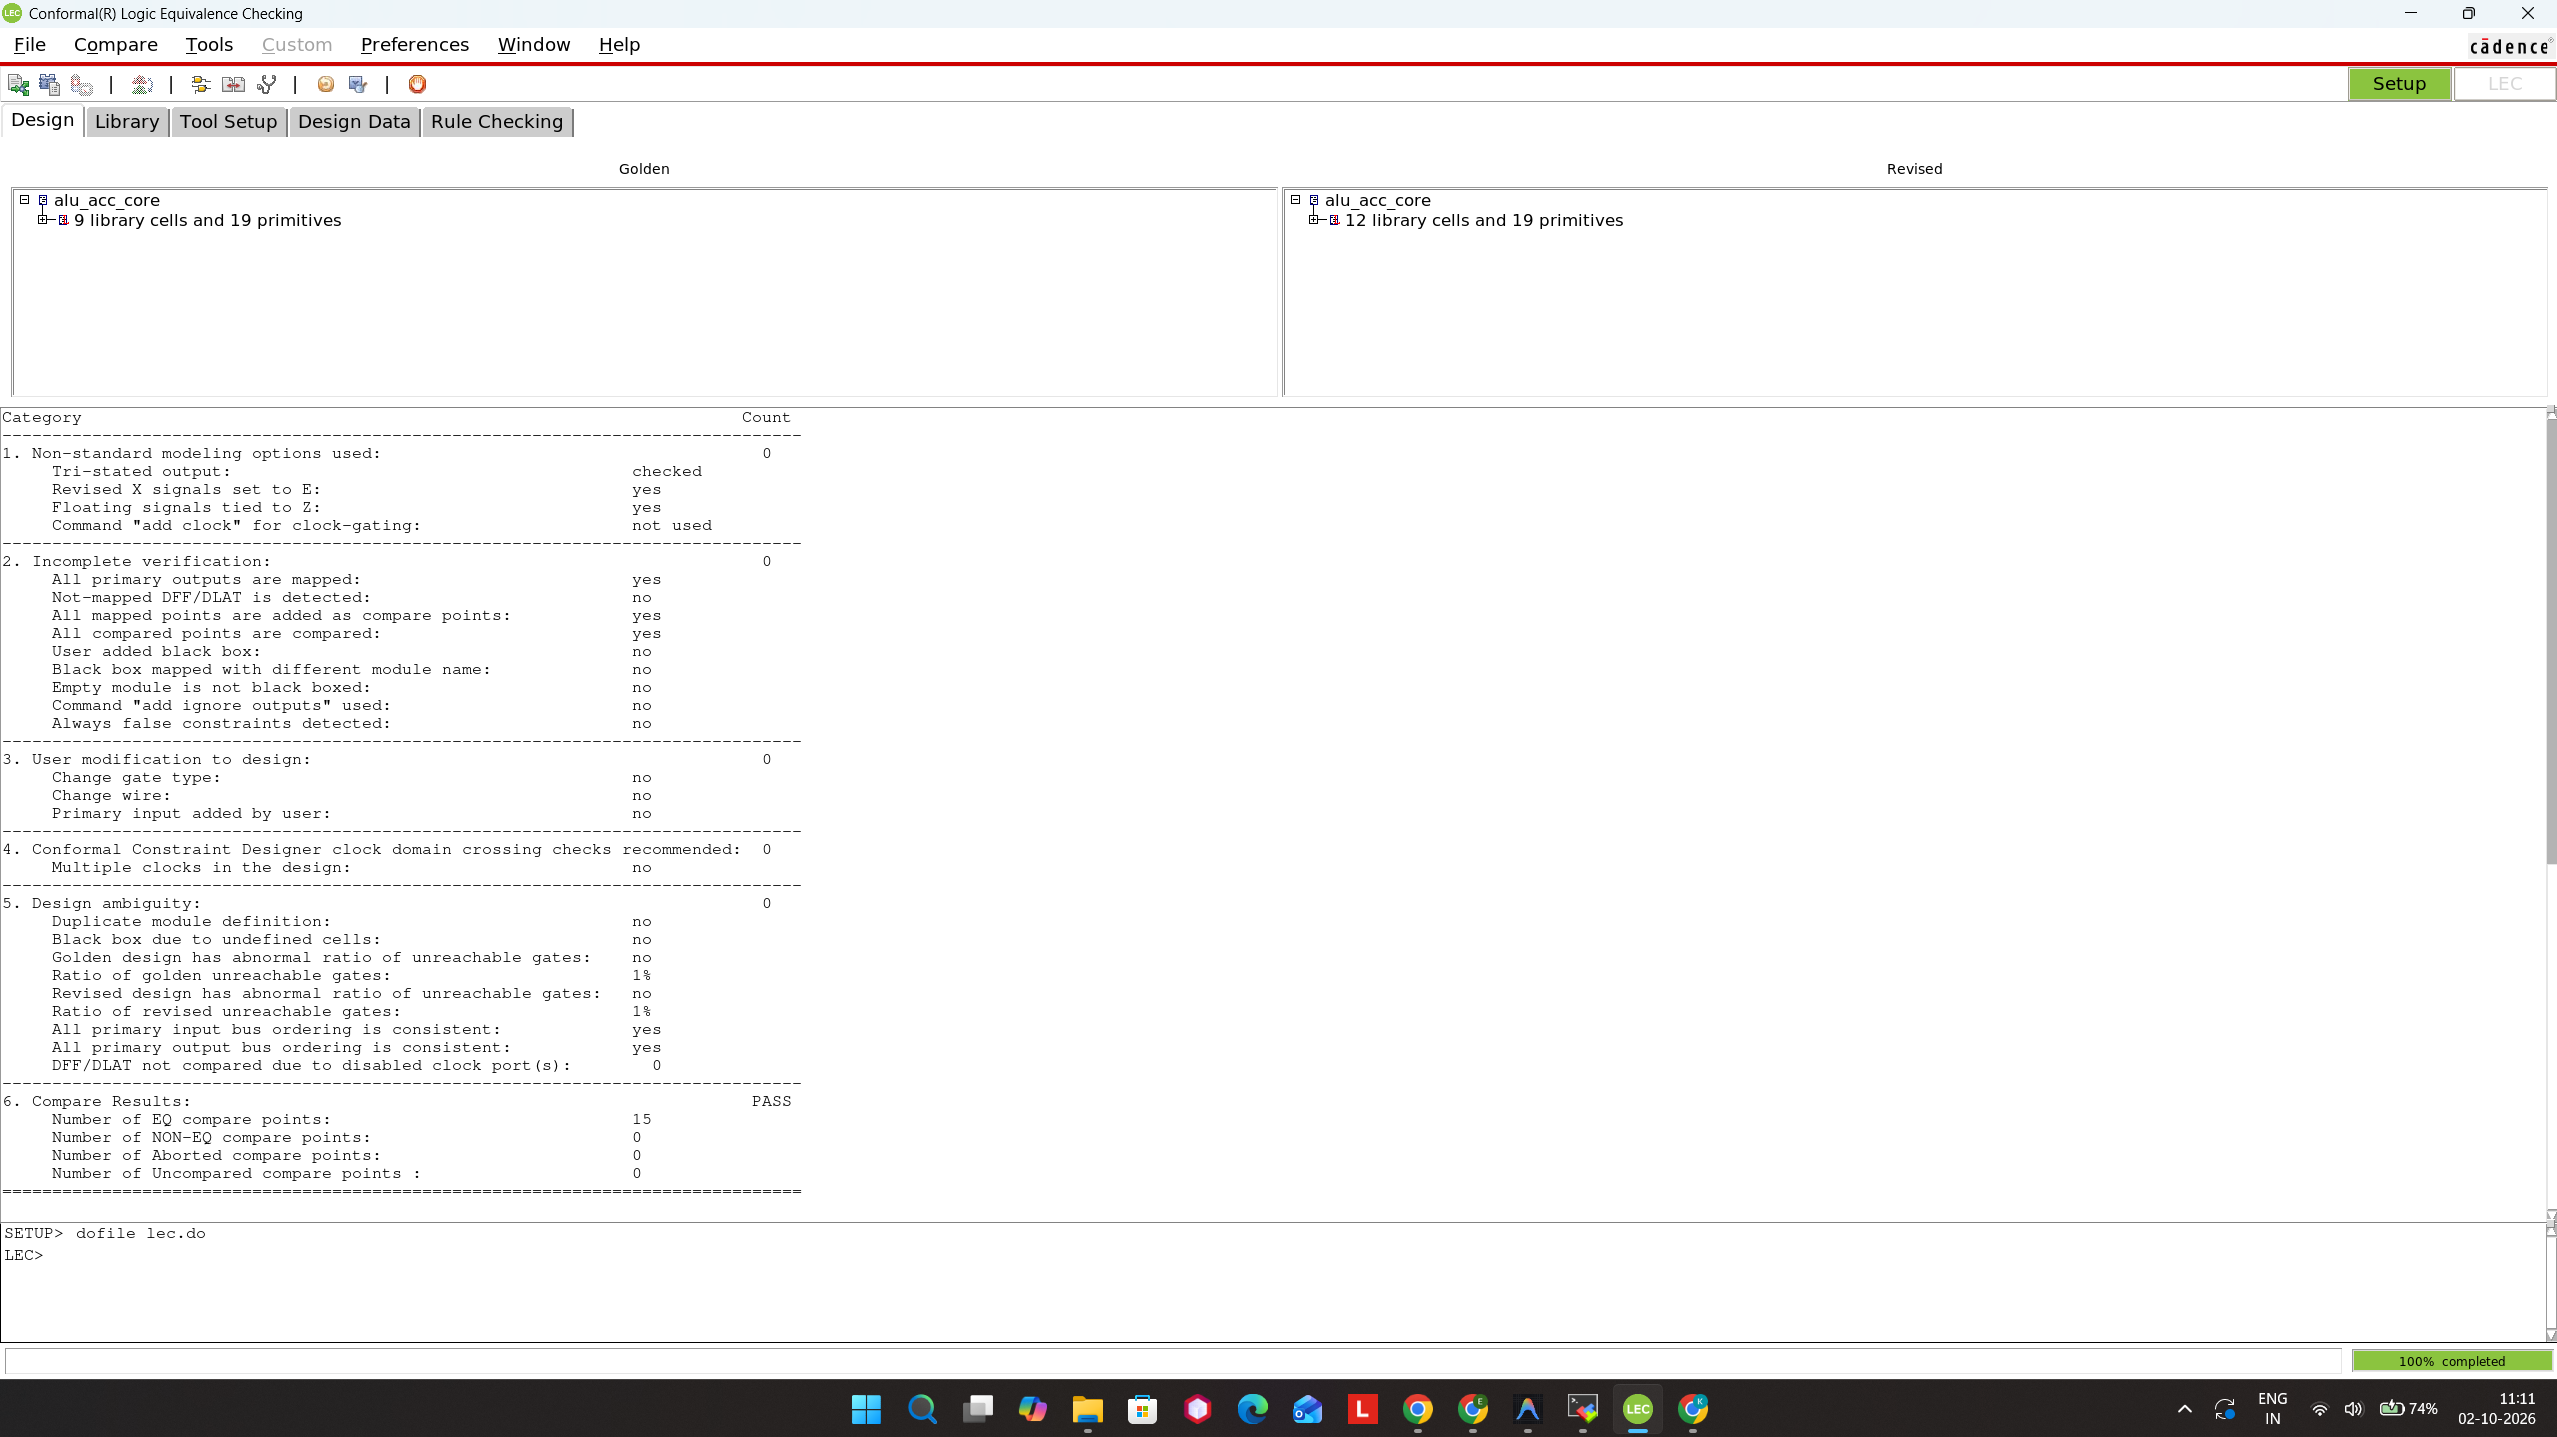
\includegraphics[width=0.8\textwidth]{Lab5_LEC_Exercises/Task1/ouput_task1.png}
    \caption{Task 1 - 100\% Equivalent (PASS)}
\end{figure}


% --- TASK 2 ---
\section{Task 2: Bitwise Operator Typo}
\textbf{Objective:} Identify and correct a logical bug in the ALU combinational logic.

\textbf{Diagnosis:} 
Conformal identified failing primary outputs. The designer accidentally used a bitwise OR operator (\texttt{|}) instead of a bitwise AND operator (\texttt{\&}) for the \texttt{and\_r} signal.

\textbf{Correction:} 
The operator was corrected in \texttt{revised\_netlist.v}.
\begin{lstlisting}[language=Verilog]
// Original Broken Code:
assign and_r=a|b;

// Corrected Code:
assign and_r=a&b;
\end{lstlisting}

\begin{figure}[H]
    \centering
    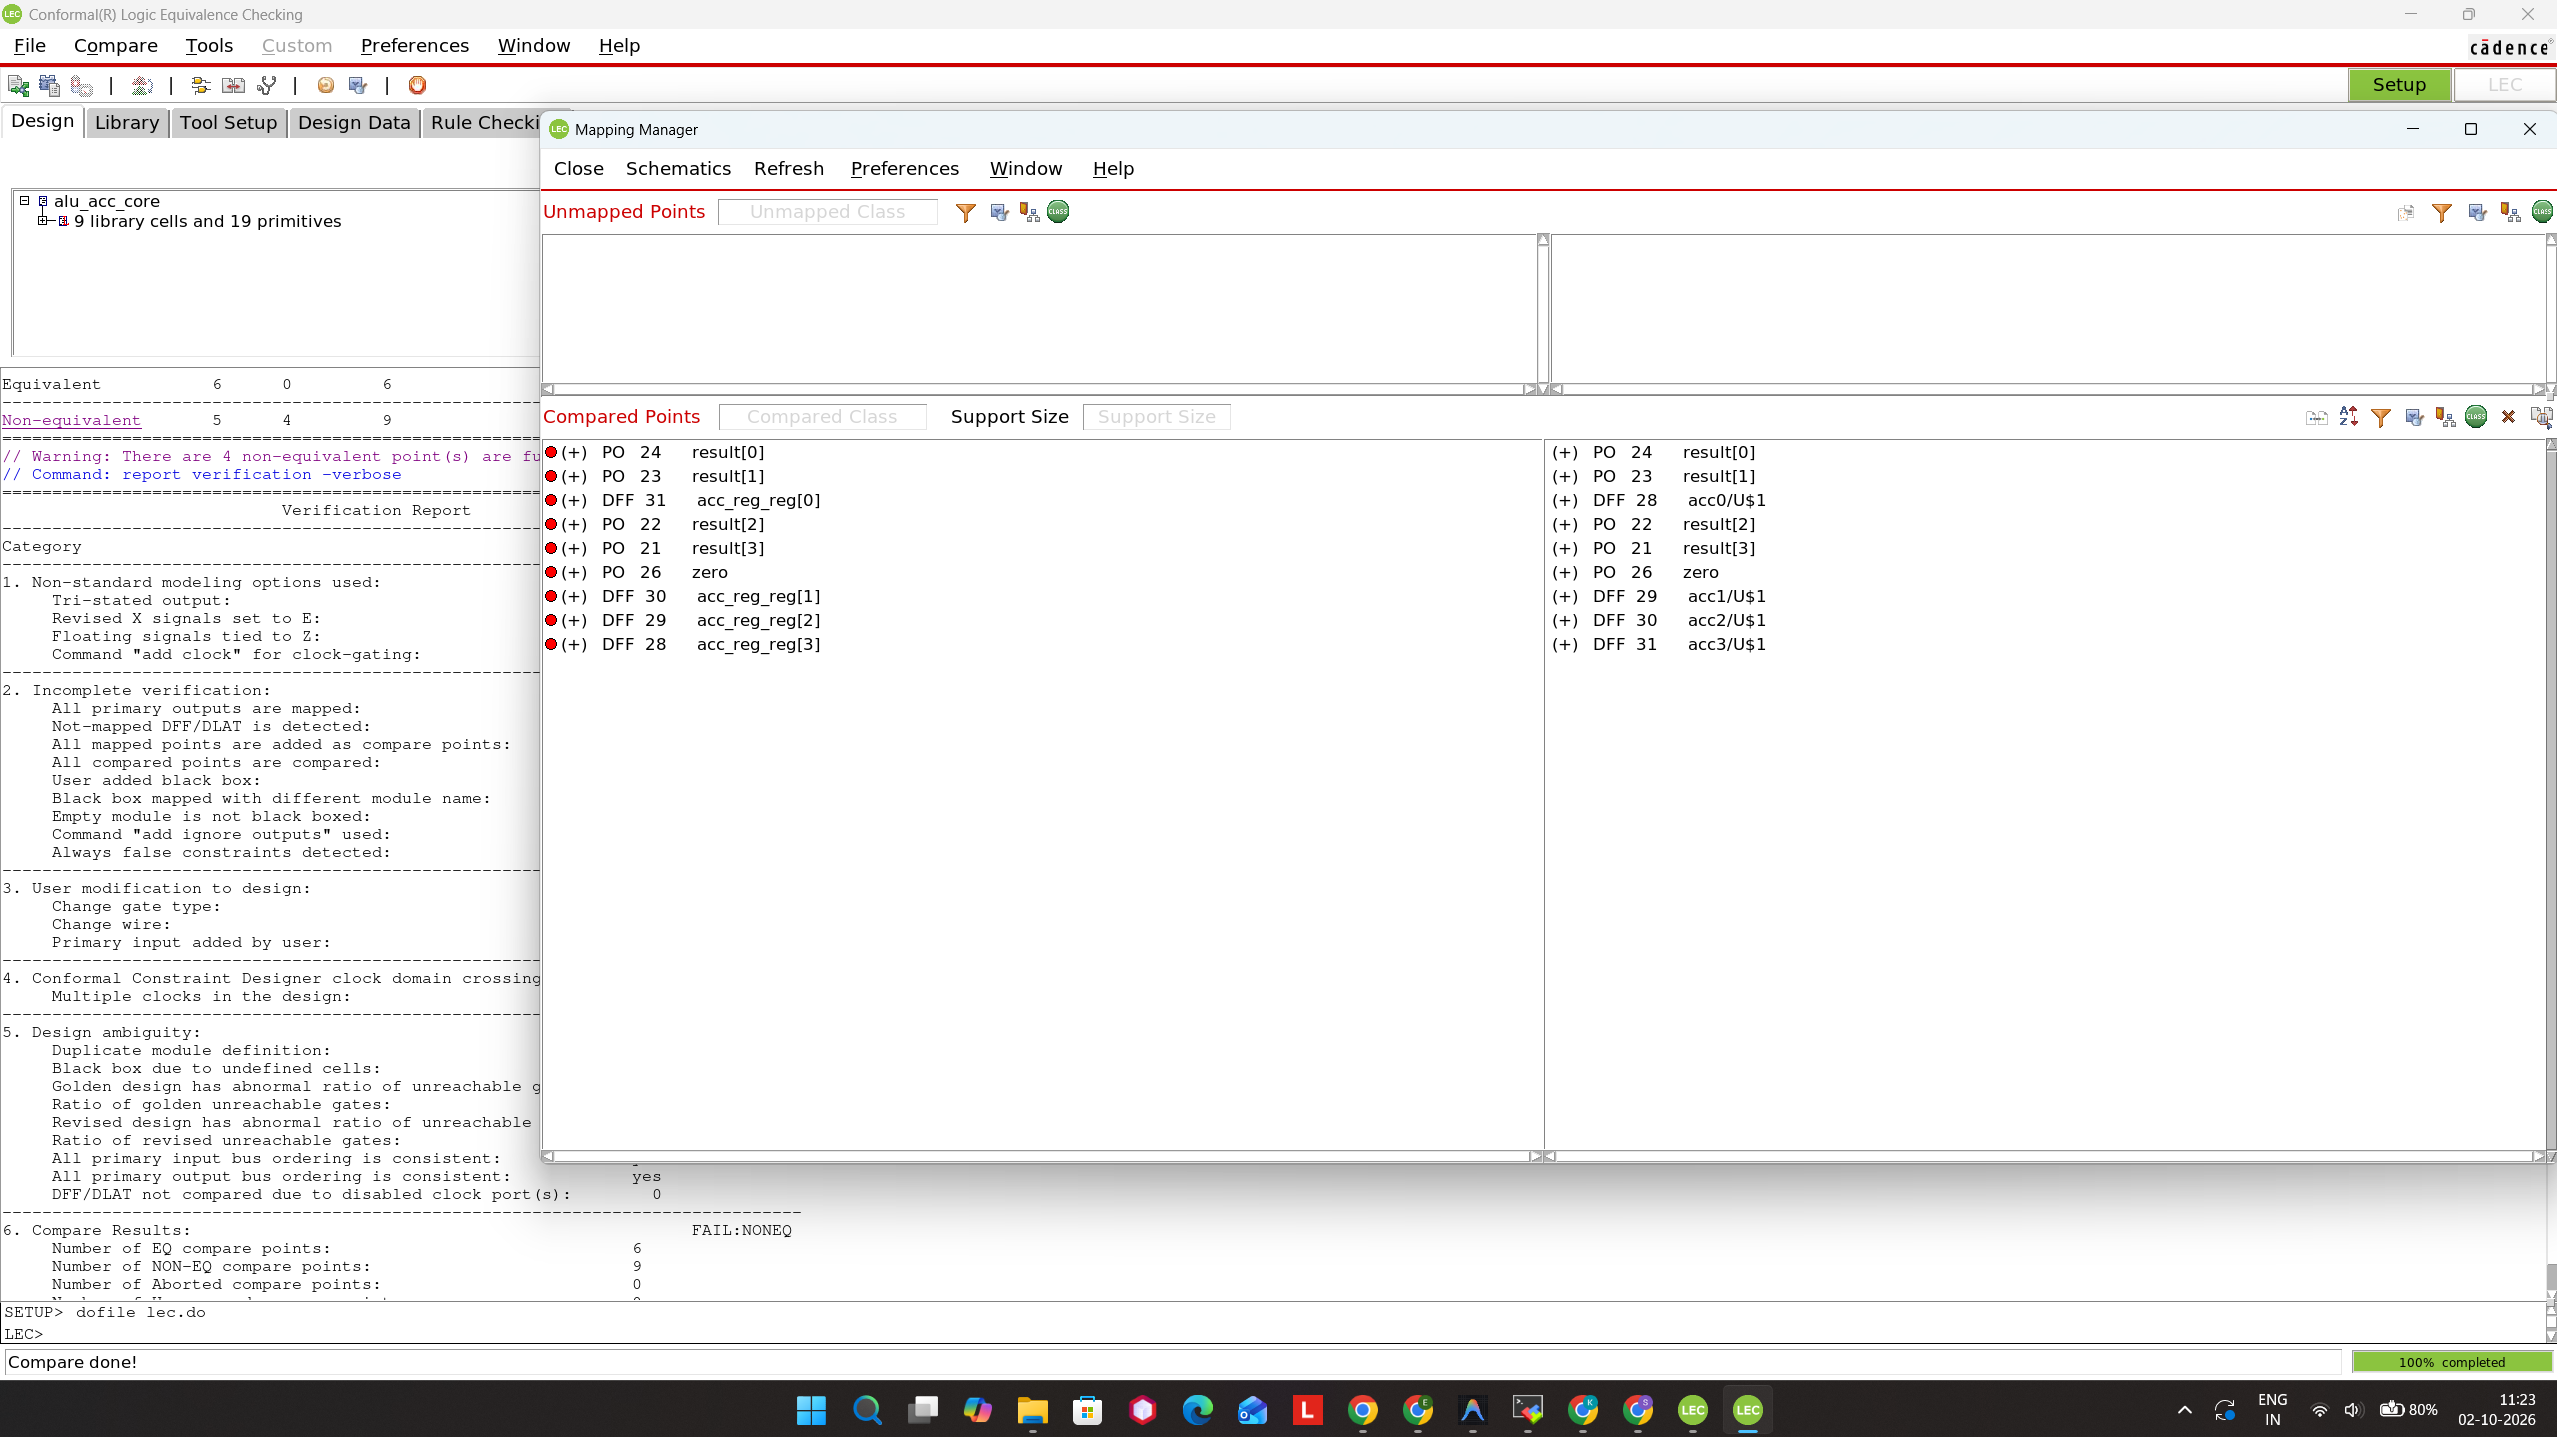
\includegraphics[width=0.8\textwidth]{Lab5_LEC_Exercises/Task2/output_taks2.png}
    \caption{Task 2 - Equivalent after correction}
\end{figure}


% --- TASK 3 ---
\section{Task 3: Multiplexer Signal Swap}
\textbf{Objective:} Debug a corrupted output caused by misrouted signals in a multiplexer.

\textbf{Diagnosis:} 
The LEC tool flagged cascading errors across \texttt{result}, \texttt{zero}, and \texttt{acc\_reg}. Diagnosing the primary output \texttt{result} revealed that the inputs to the output multiplexer for opcodes \texttt{10} and \texttt{11} were swapped.

\begin{figure}[H]
    \centering
    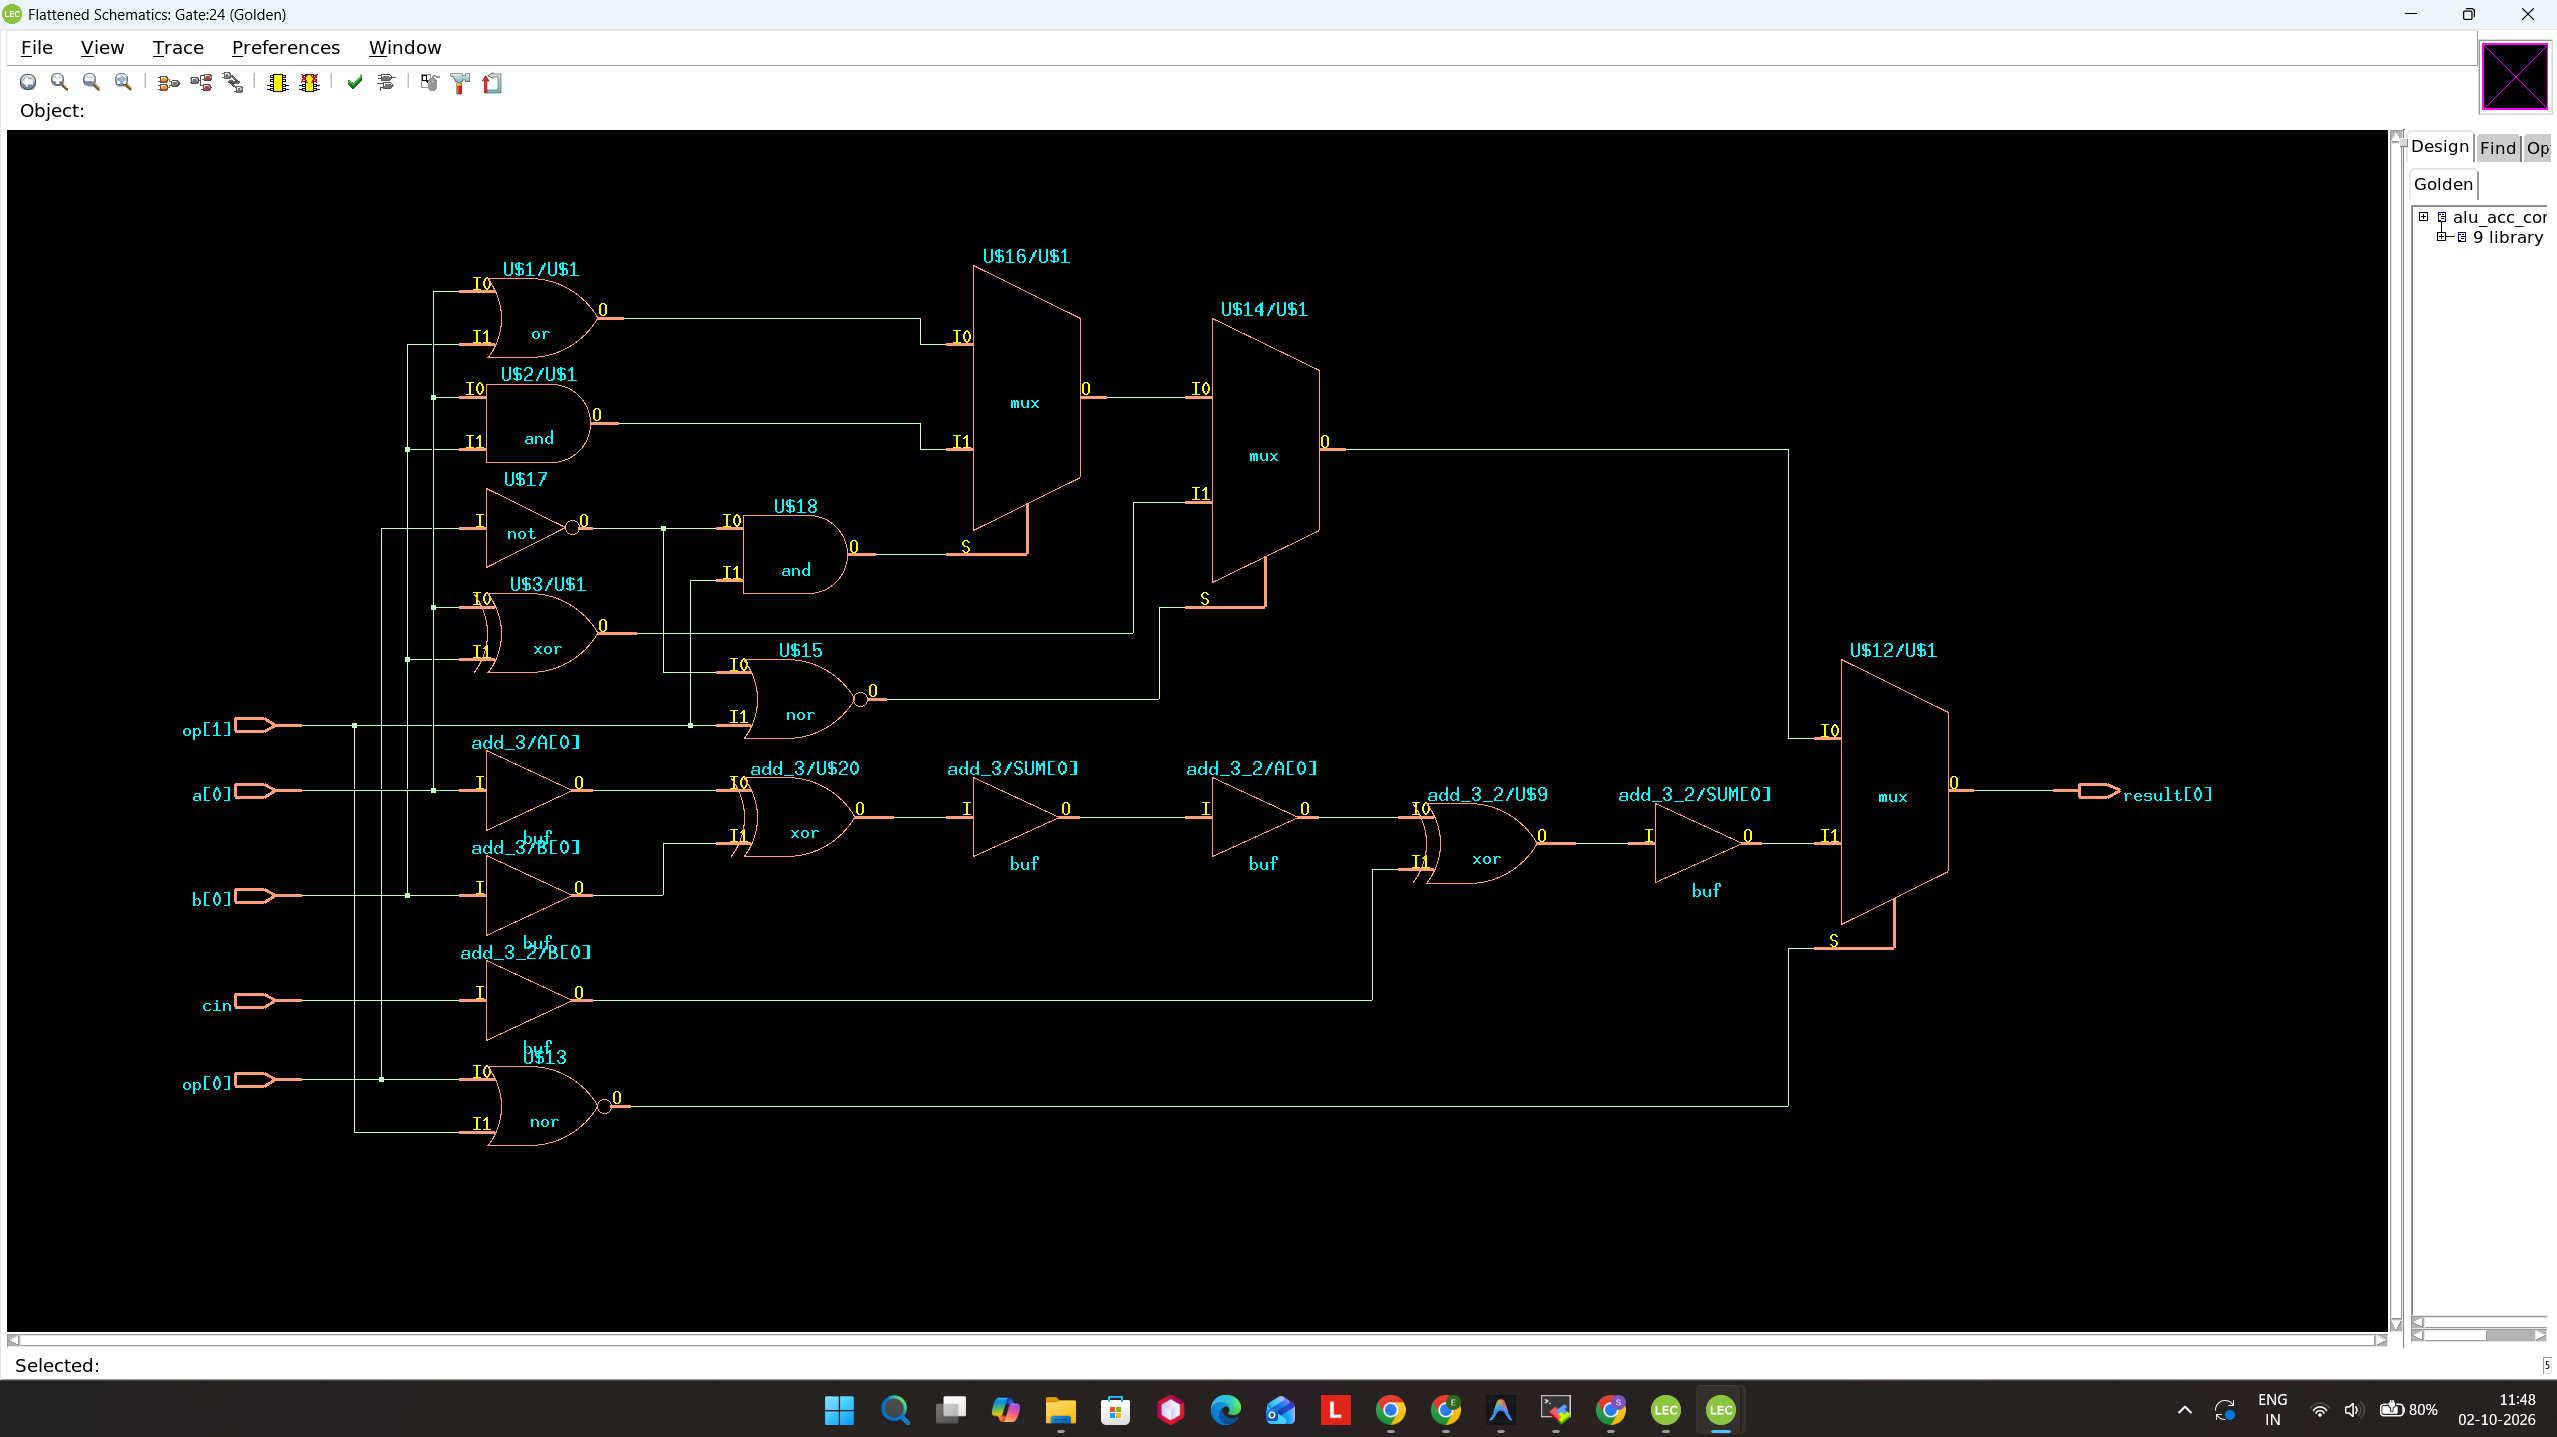
\includegraphics[width=0.8\textwidth]{Lab5_LEC_Exercises/Task3/output_task_3_golden.png}
    \caption{Task 3 - Golden Schematic}
\end{figure}
\begin{figure}[H]
    \centering
    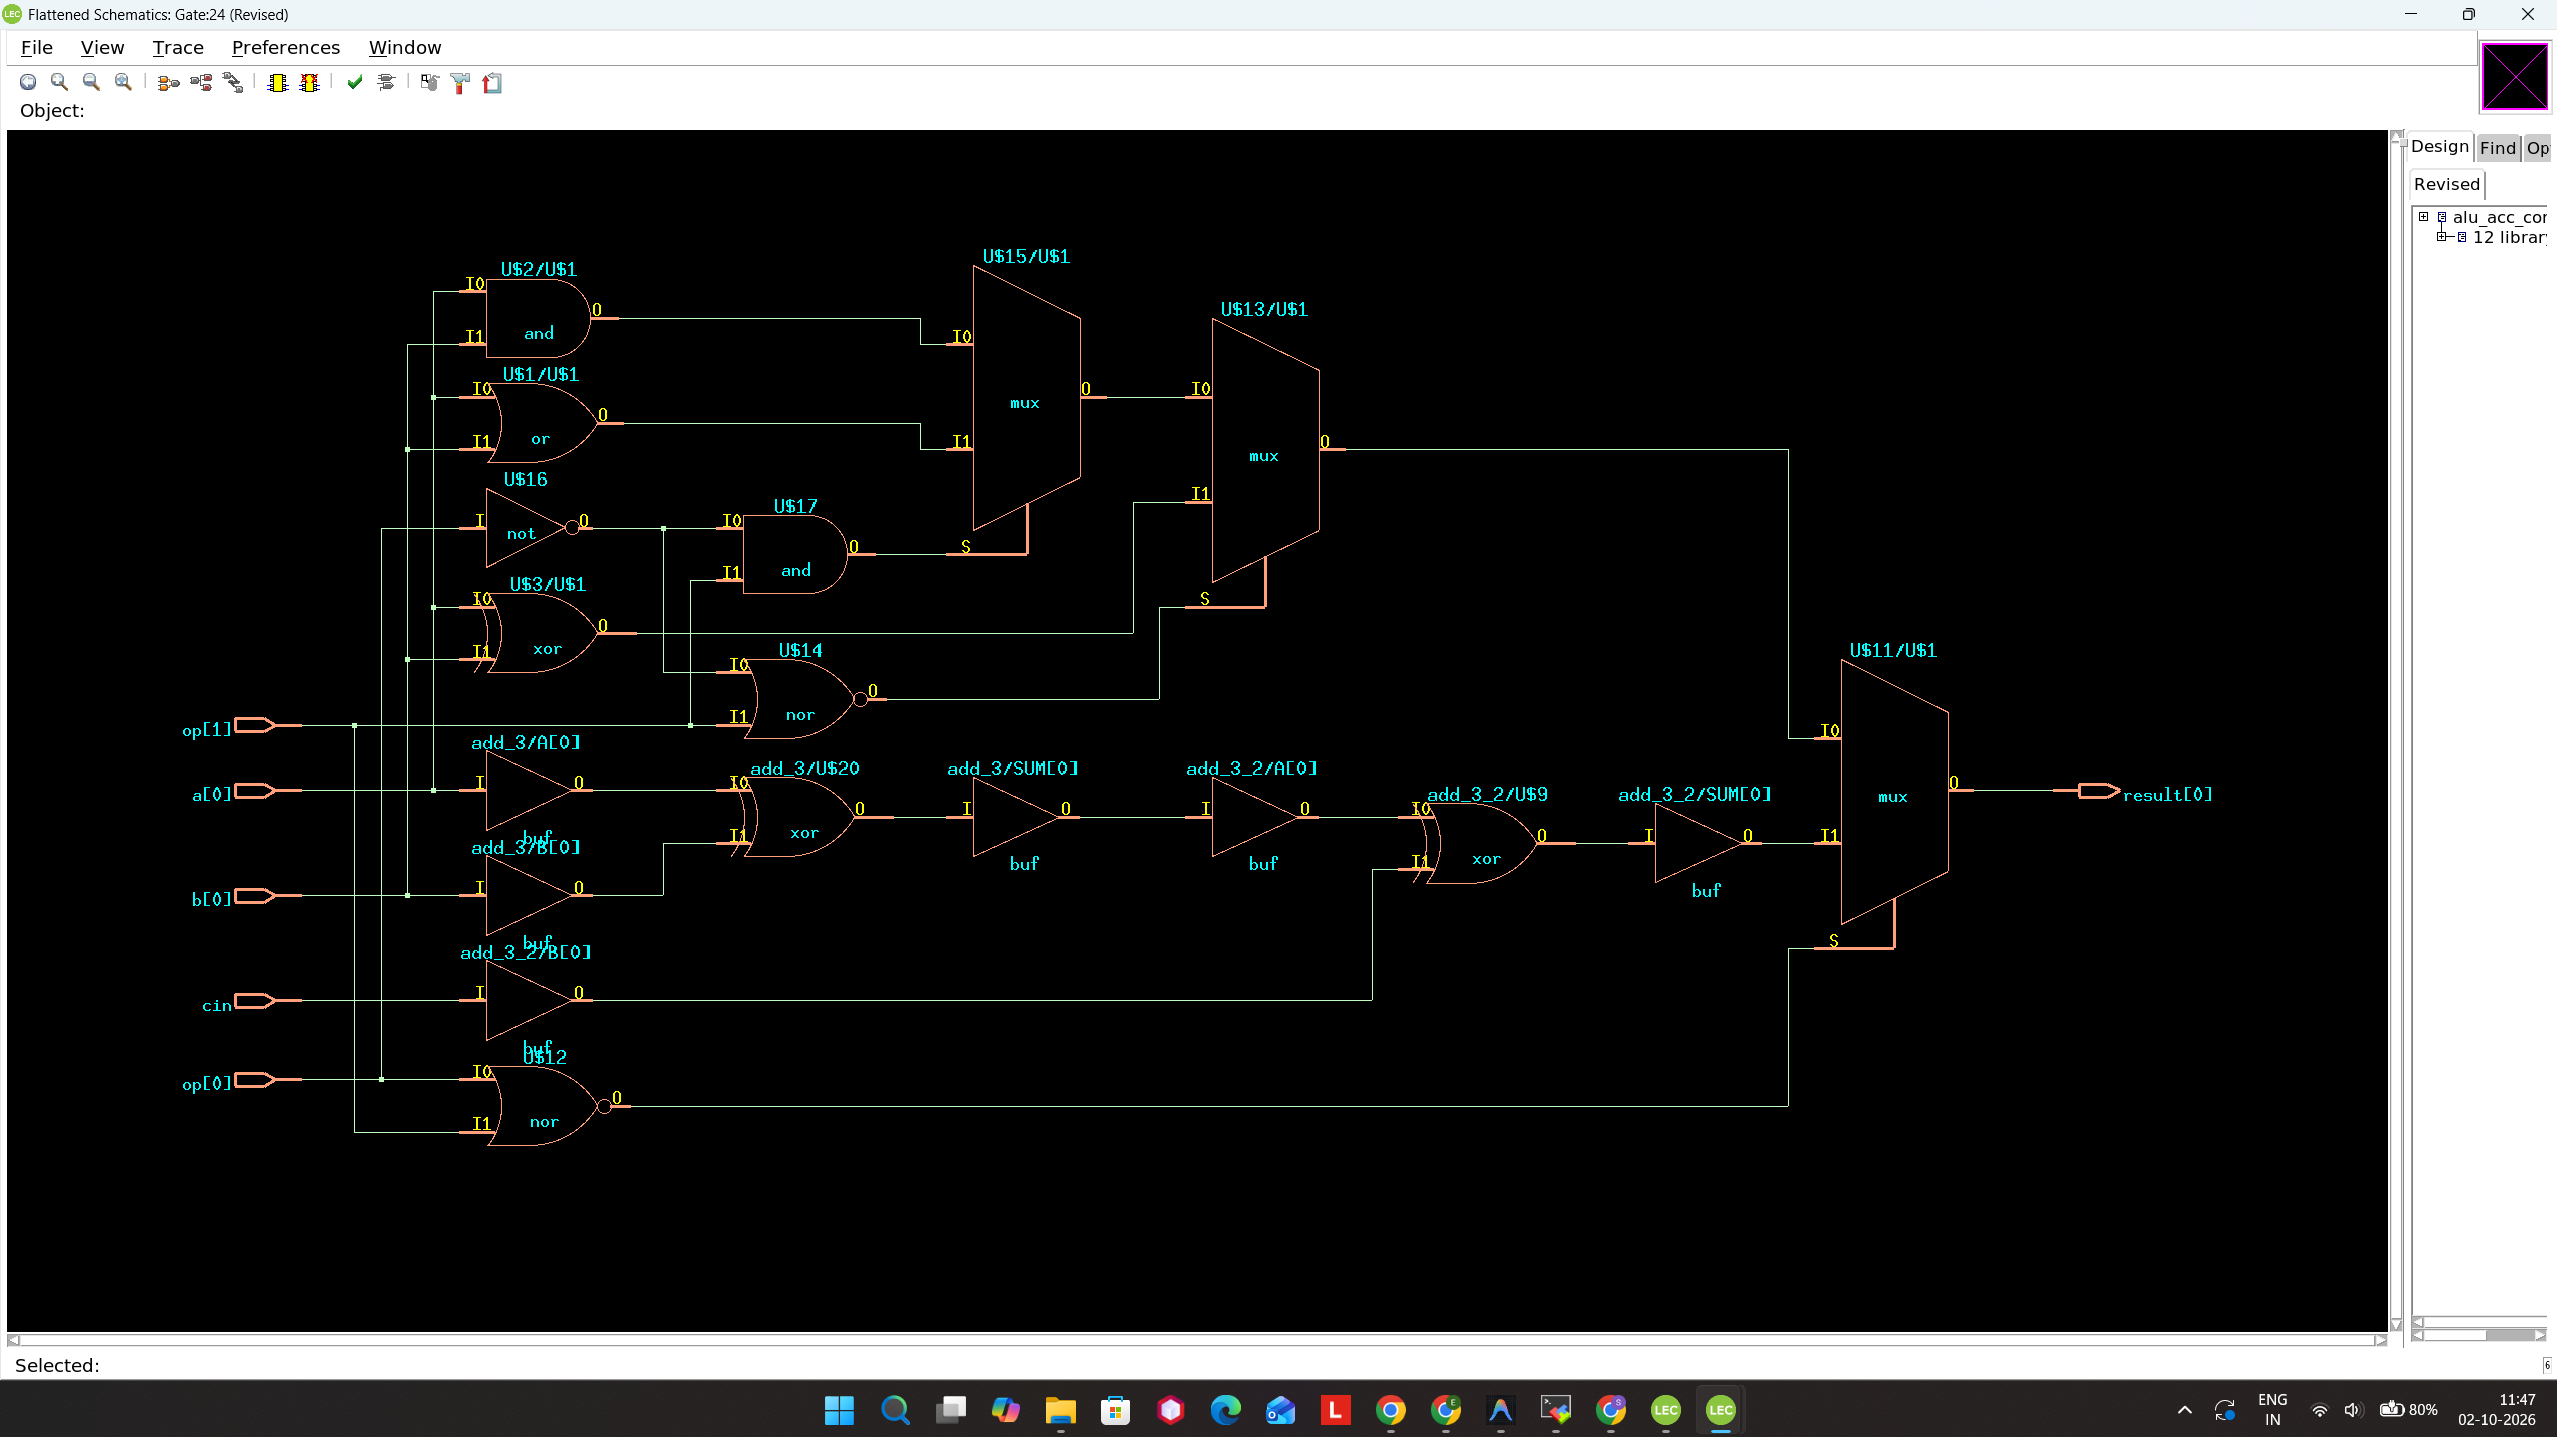
\includegraphics[width=0.8\textwidth]{Lab5_LEC_Exercises/Task3/output_task_3_revised.png}
    \caption{Task 3 - Revised Schematic showing swapped wires}
\end{figure}

\textbf{Correction:} 
\begin{lstlisting}[language=Verilog]
// Original Broken Code:
assign result=(op==2'b00)?add_r:(op==2'b01)?xor_r:(op==2'b10)?or_r:and_r;

// Corrected Code:
assign result=(op==2'b00)?add_r:(op==2'b01)?xor_r:(op==2'b10)?and_r:or_r;
\end{lstlisting}

\begin{figure}[H]
    \centering
    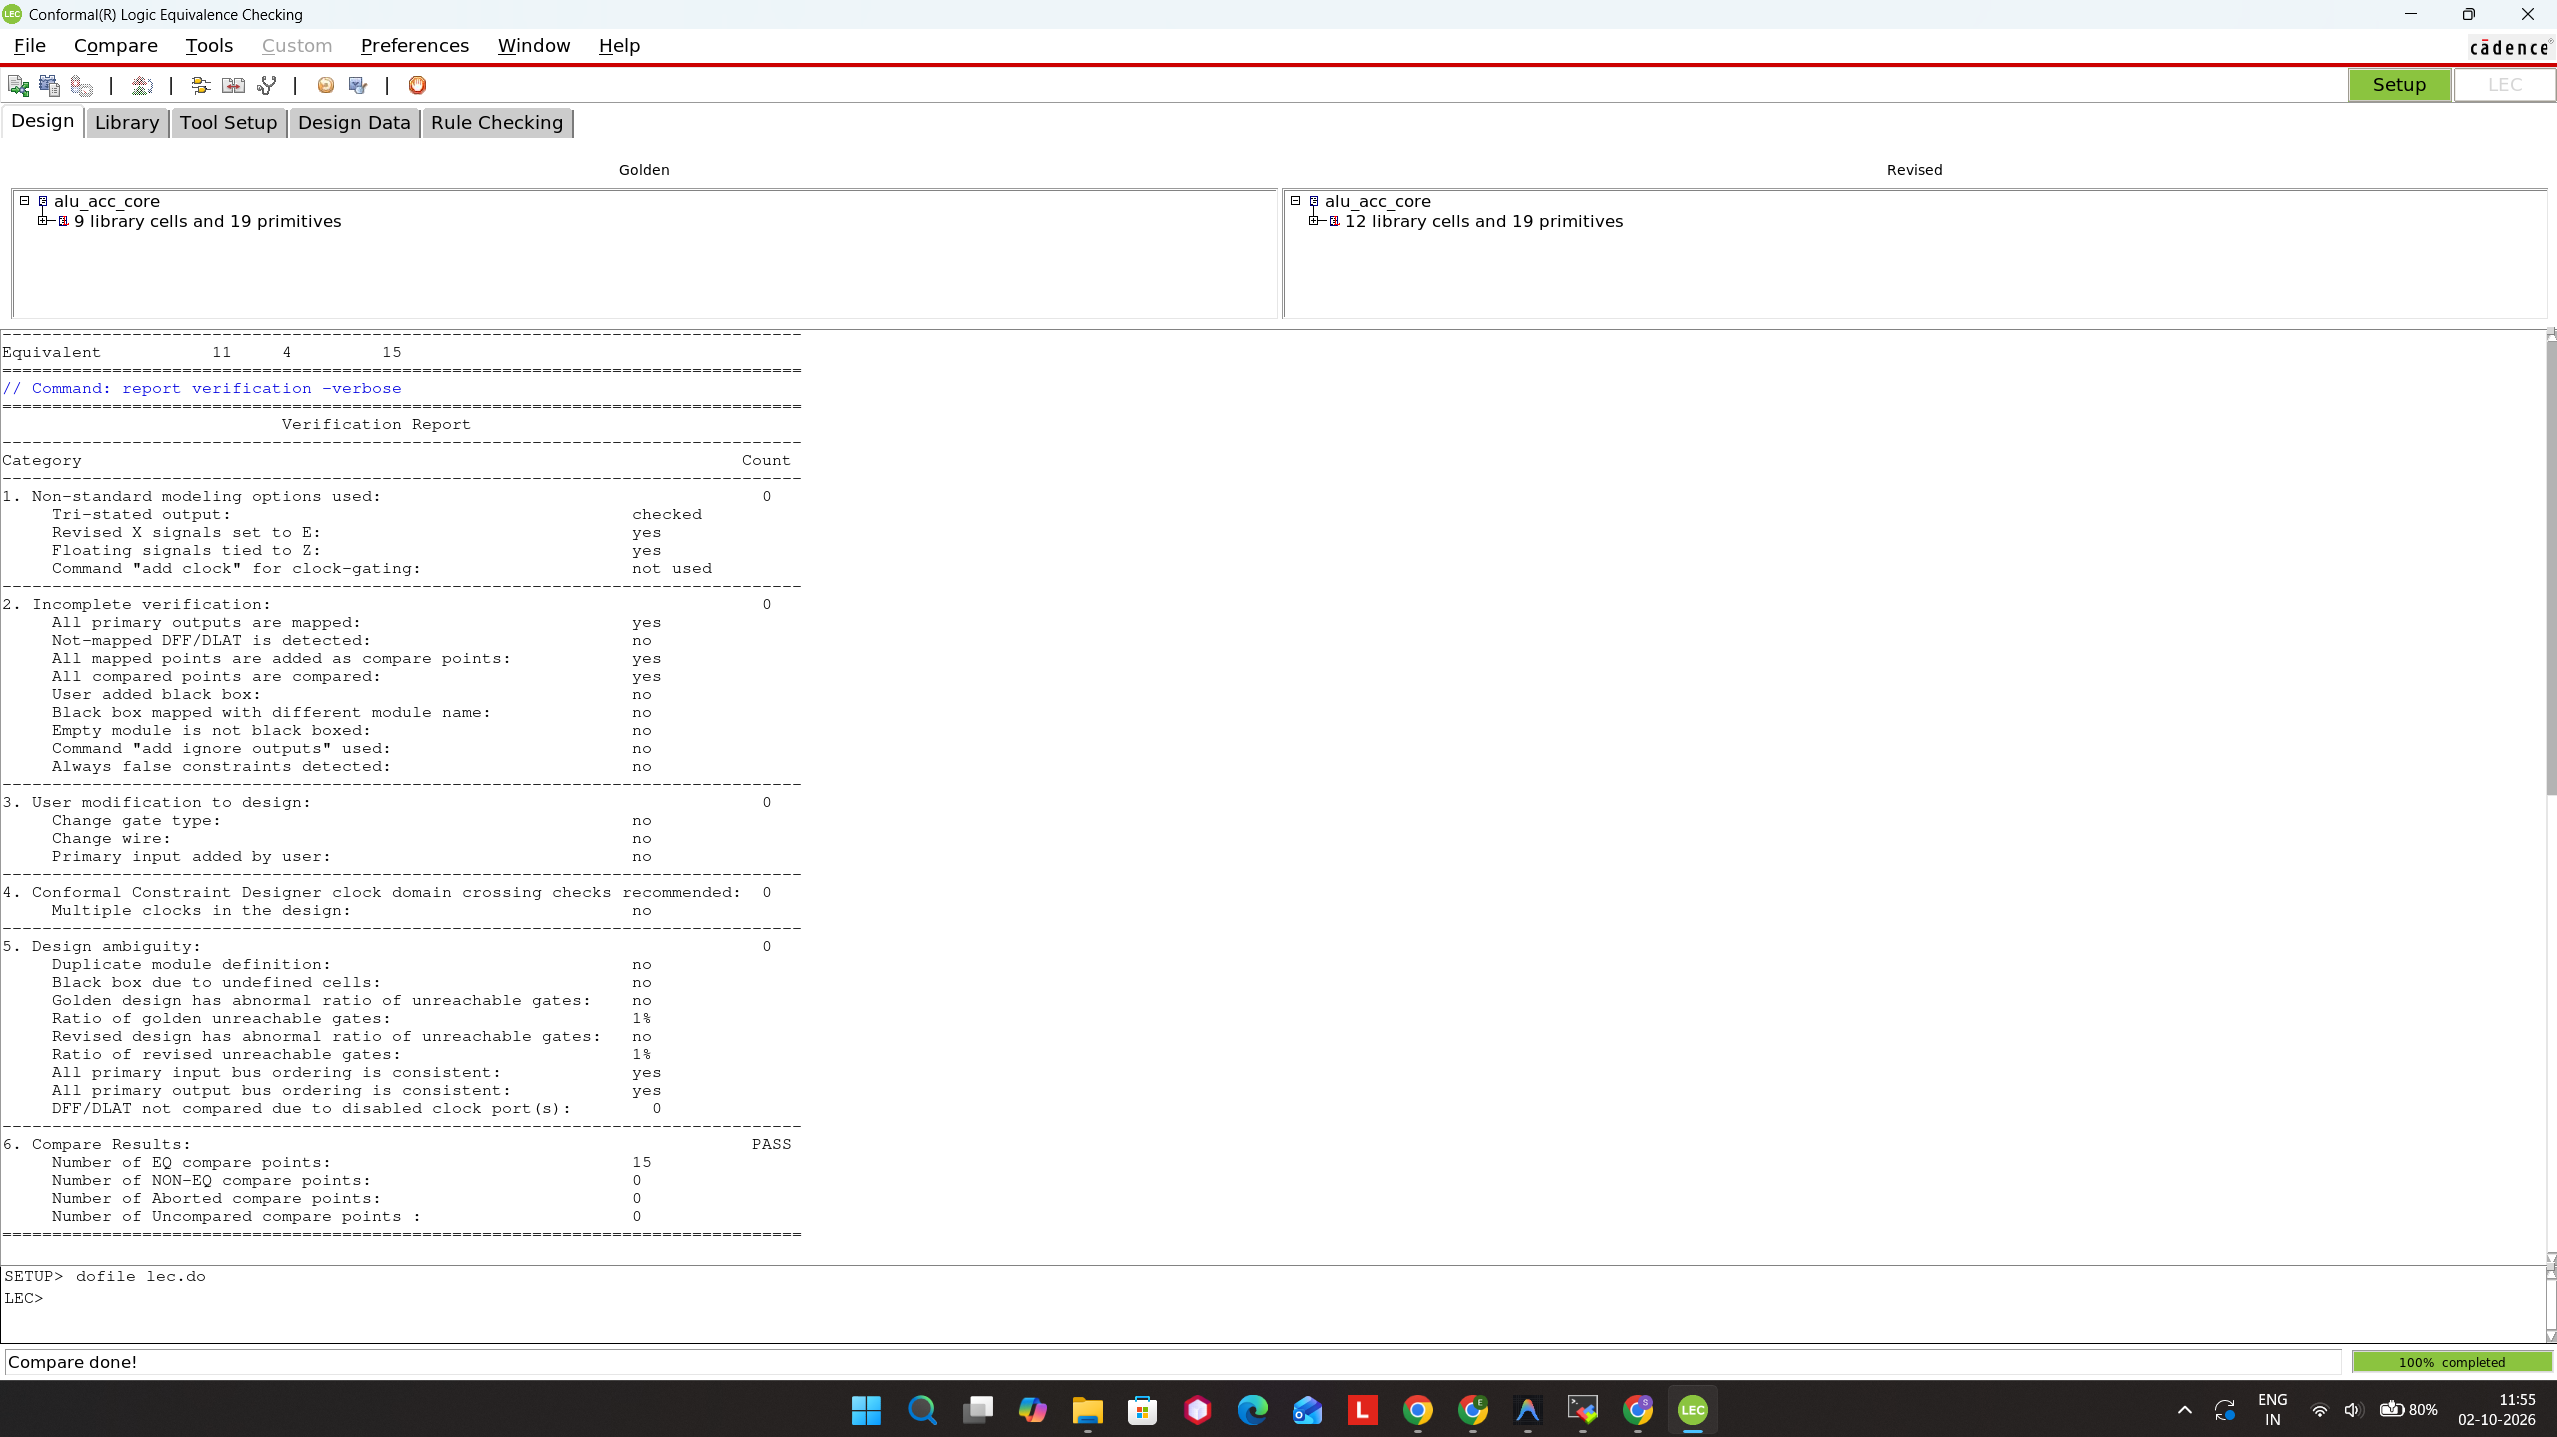
\includegraphics[width=0.8\textwidth]{Lab5_LEC_Exercises/Task3/output_task_3_lec_passed.png}
    \caption{Task 3 - PASS after correction}
\end{figure}


% --- TASK 4 ---
\section{Task 4: Missing Enable Logic on Flip-Flops}
\textbf{Objective:} Identify missing sequential logic controlling the flip-flops.

\textbf{Diagnosis:} 
The primary outputs passed, but all 4 \texttt{acc\_reg} flip-flops failed. The Golden design used a multiplexer to loop the output back into the flip-flop when the \texttt{en} signal was 0. The Revised design ignored this completely.

\begin{figure}[H]
    \centering
    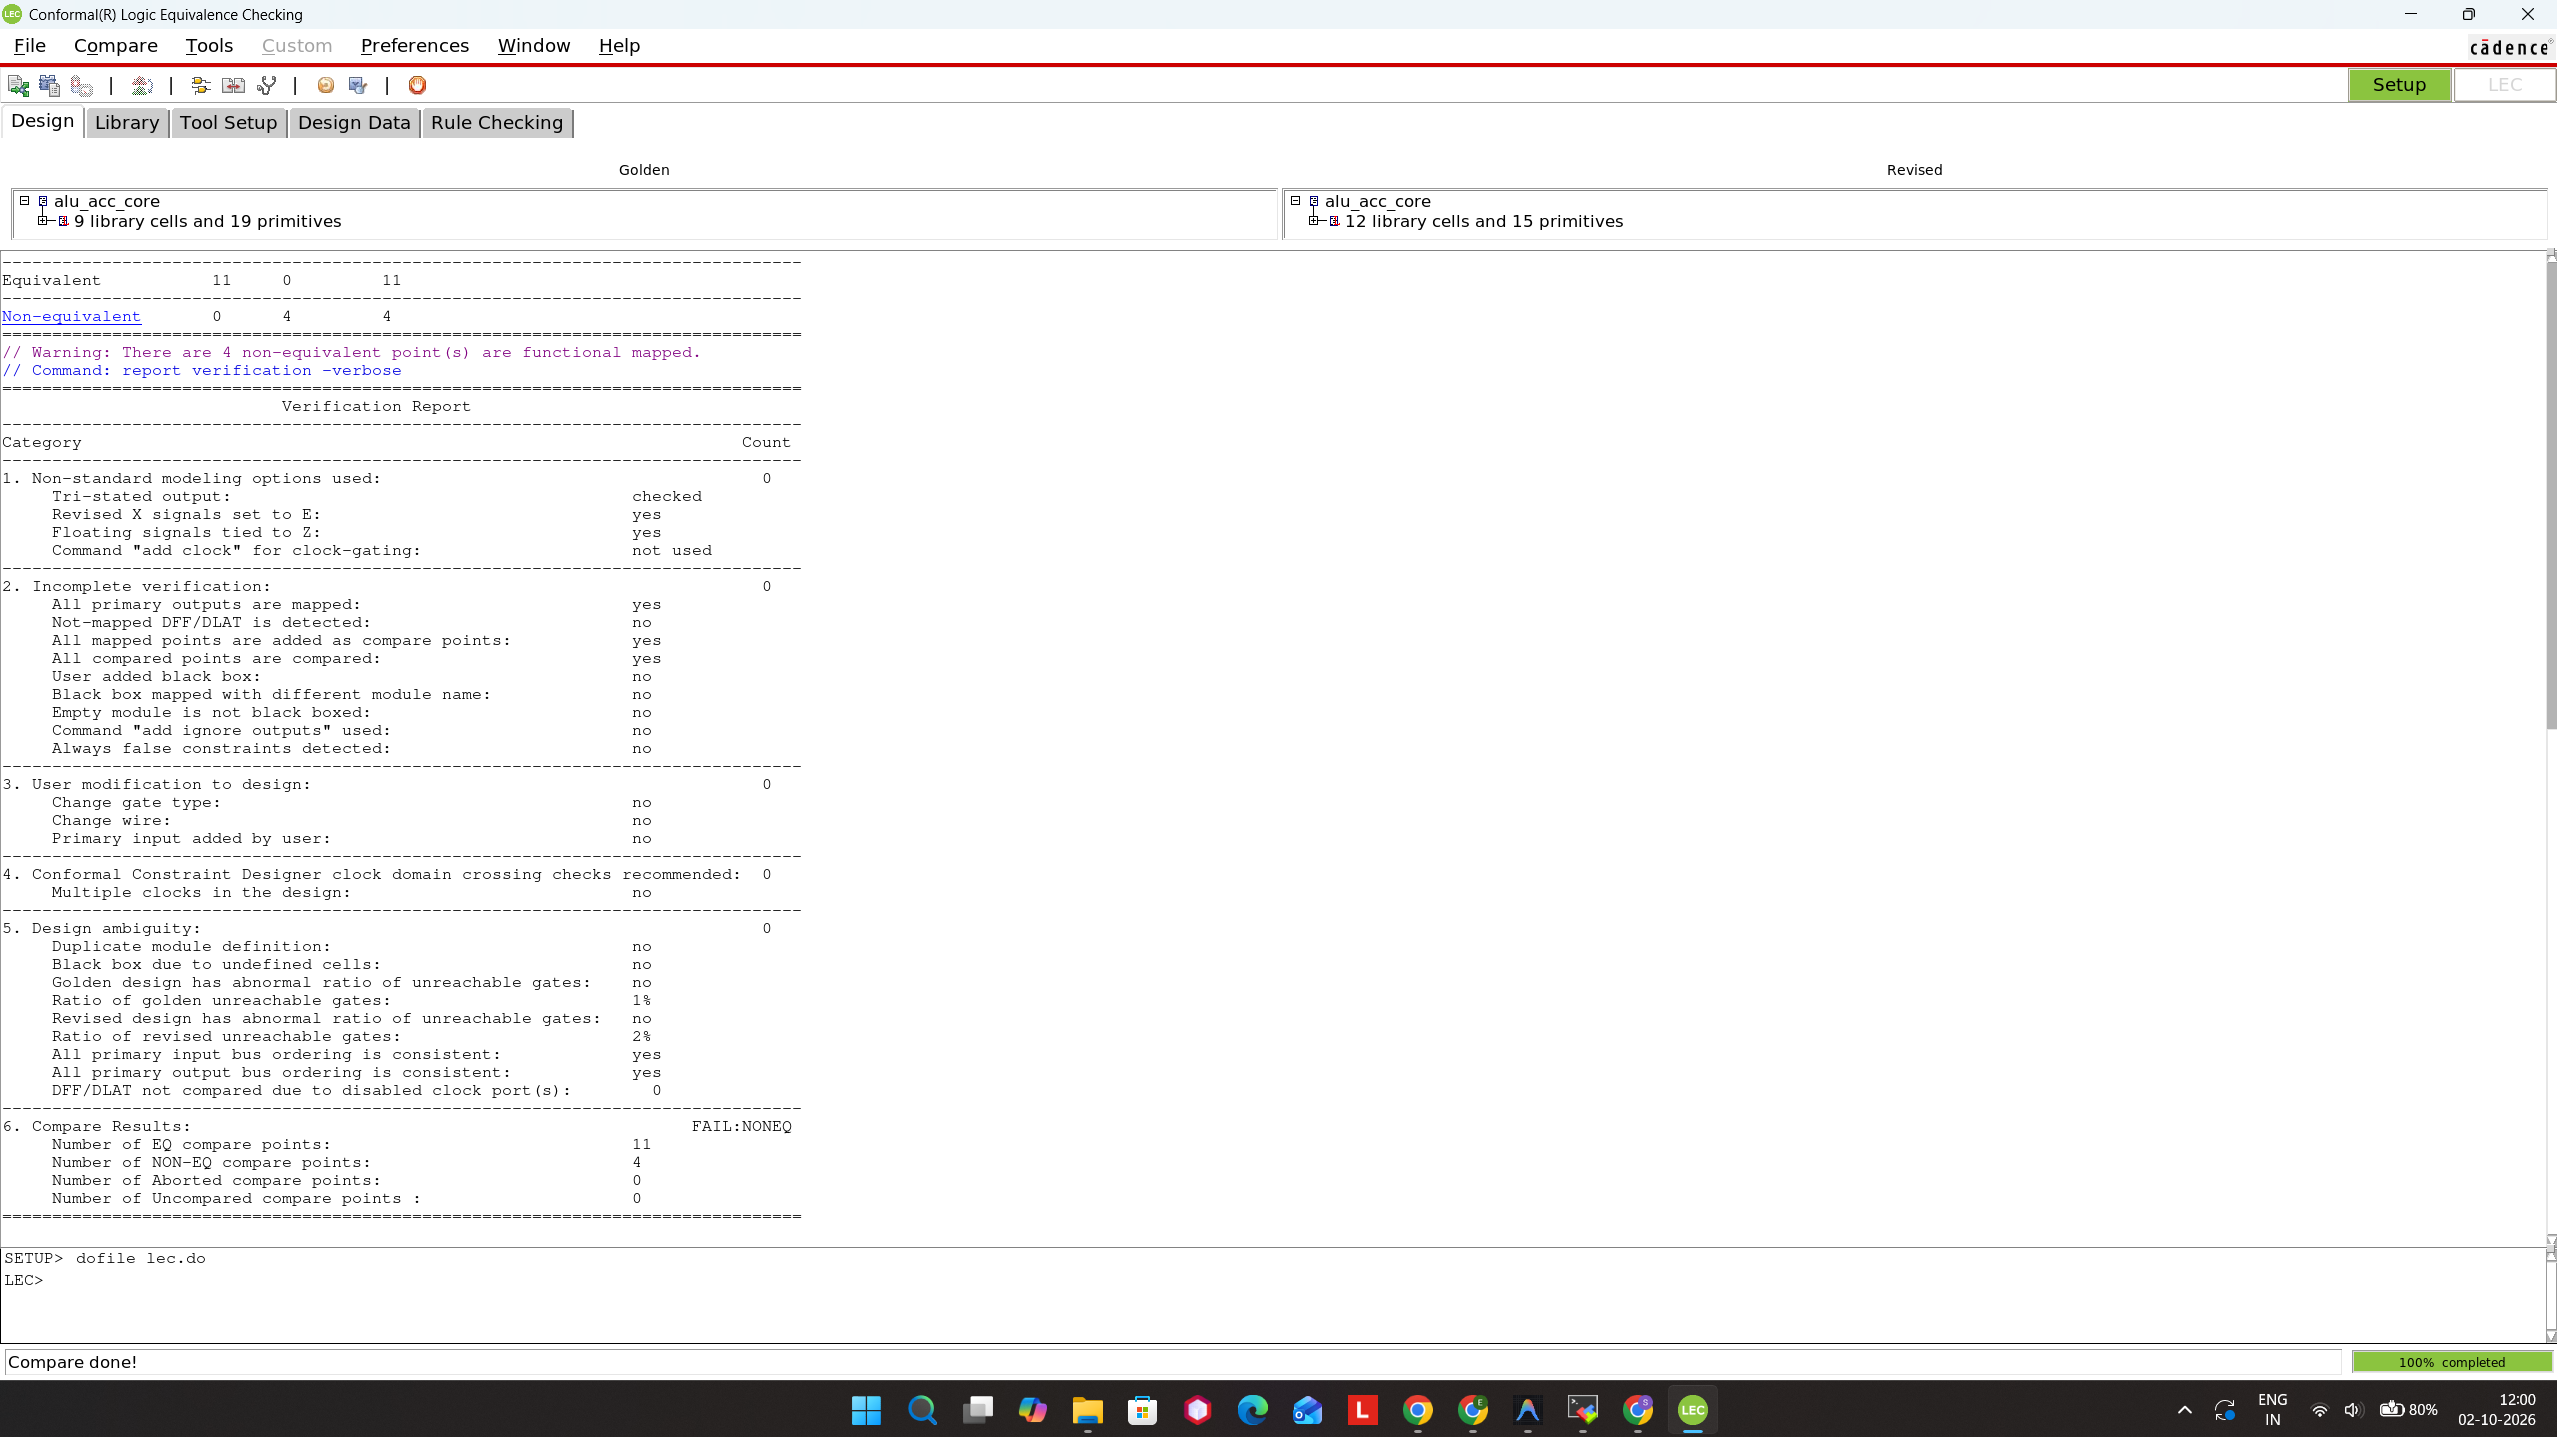
\includegraphics[width=0.8\textwidth]{Lab5_LEC_Exercises/Task4/output_task4.png}
    \caption{Task 4 - Failing Flip-Flops in Mapping Manager}
\end{figure}

\begin{figure}[H]
    \centering
    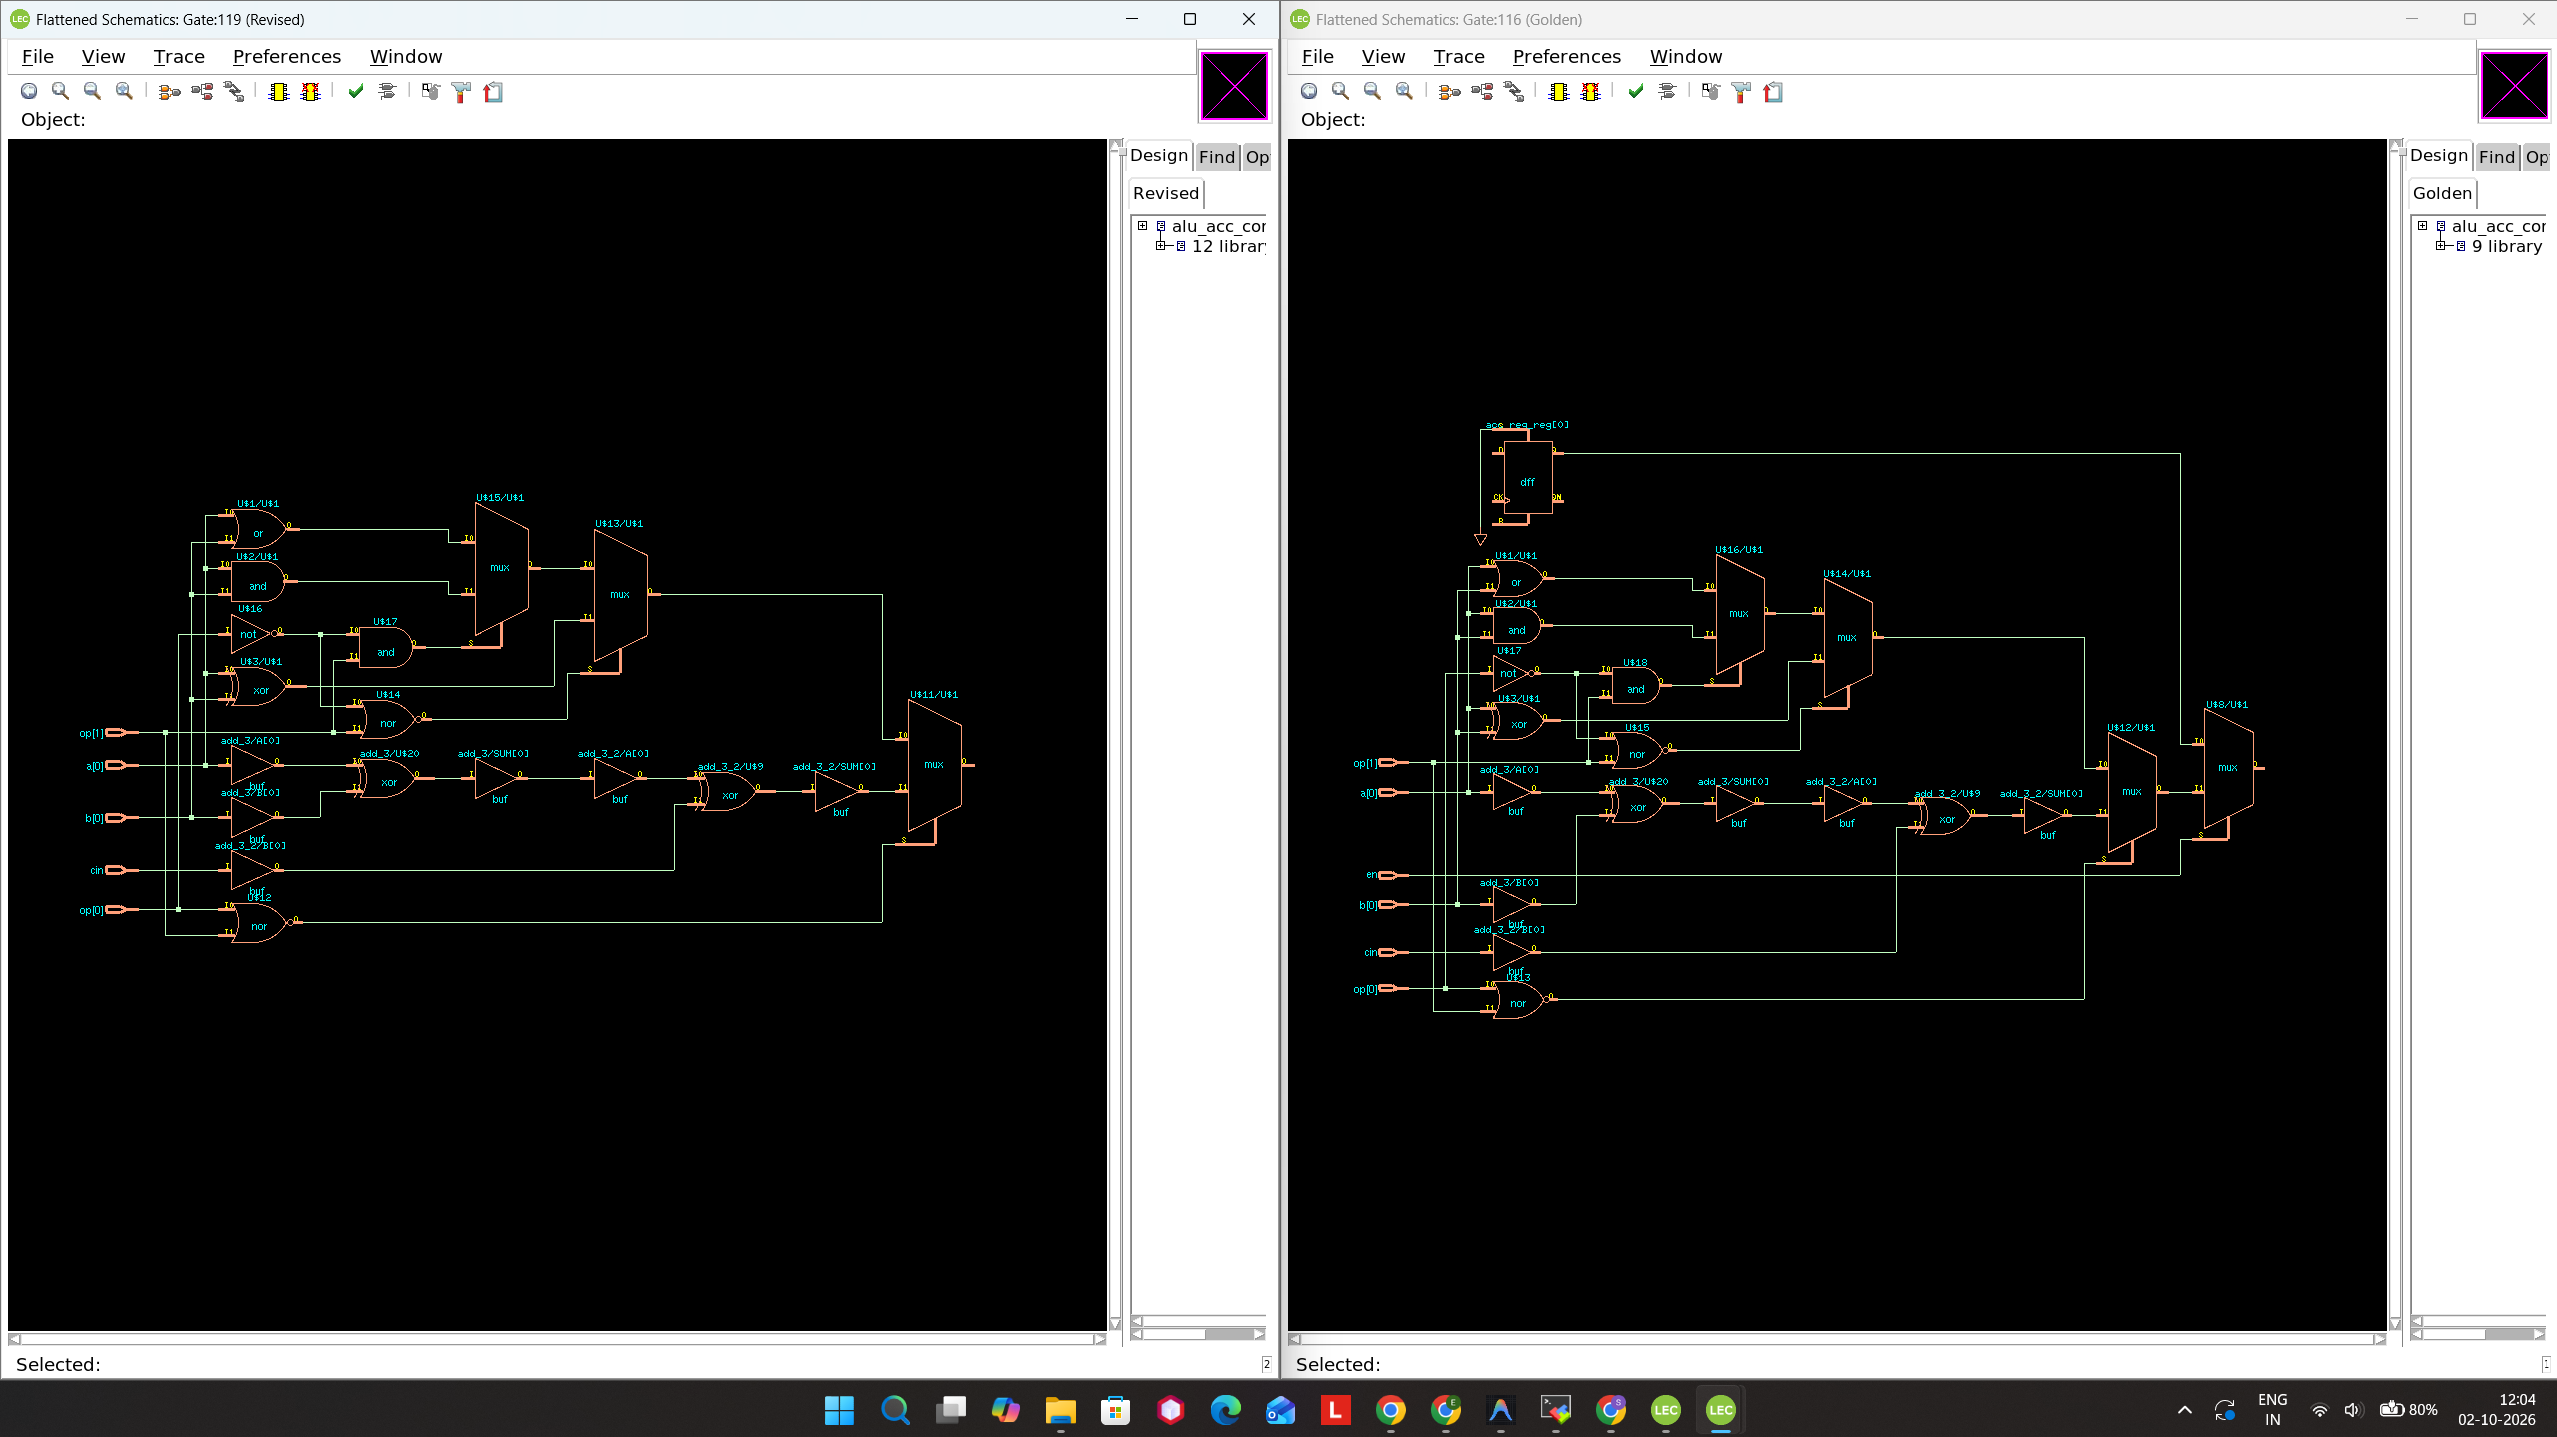
\includegraphics[width=0.8\textwidth]{Lab5_LEC_Exercises/Task4/golden_revised_comparion_task4.png}
    \caption{Task 4 - Schematic showing missing enable MUX in Revised}
\end{figure}

\textbf{Correction:} 
A ternary operator was added to the \texttt{.D} pin of all 4 flip-flops.
\begin{lstlisting}[language=Verilog]
// Corrected Code:
DFFRX1 acc0(.D(en?result[0]:acc_reg[0]),.RN(rst_n),.CK(clk),.Q(acc_reg[0]));
\end{lstlisting}

\begin{figure}[H]
    \centering
    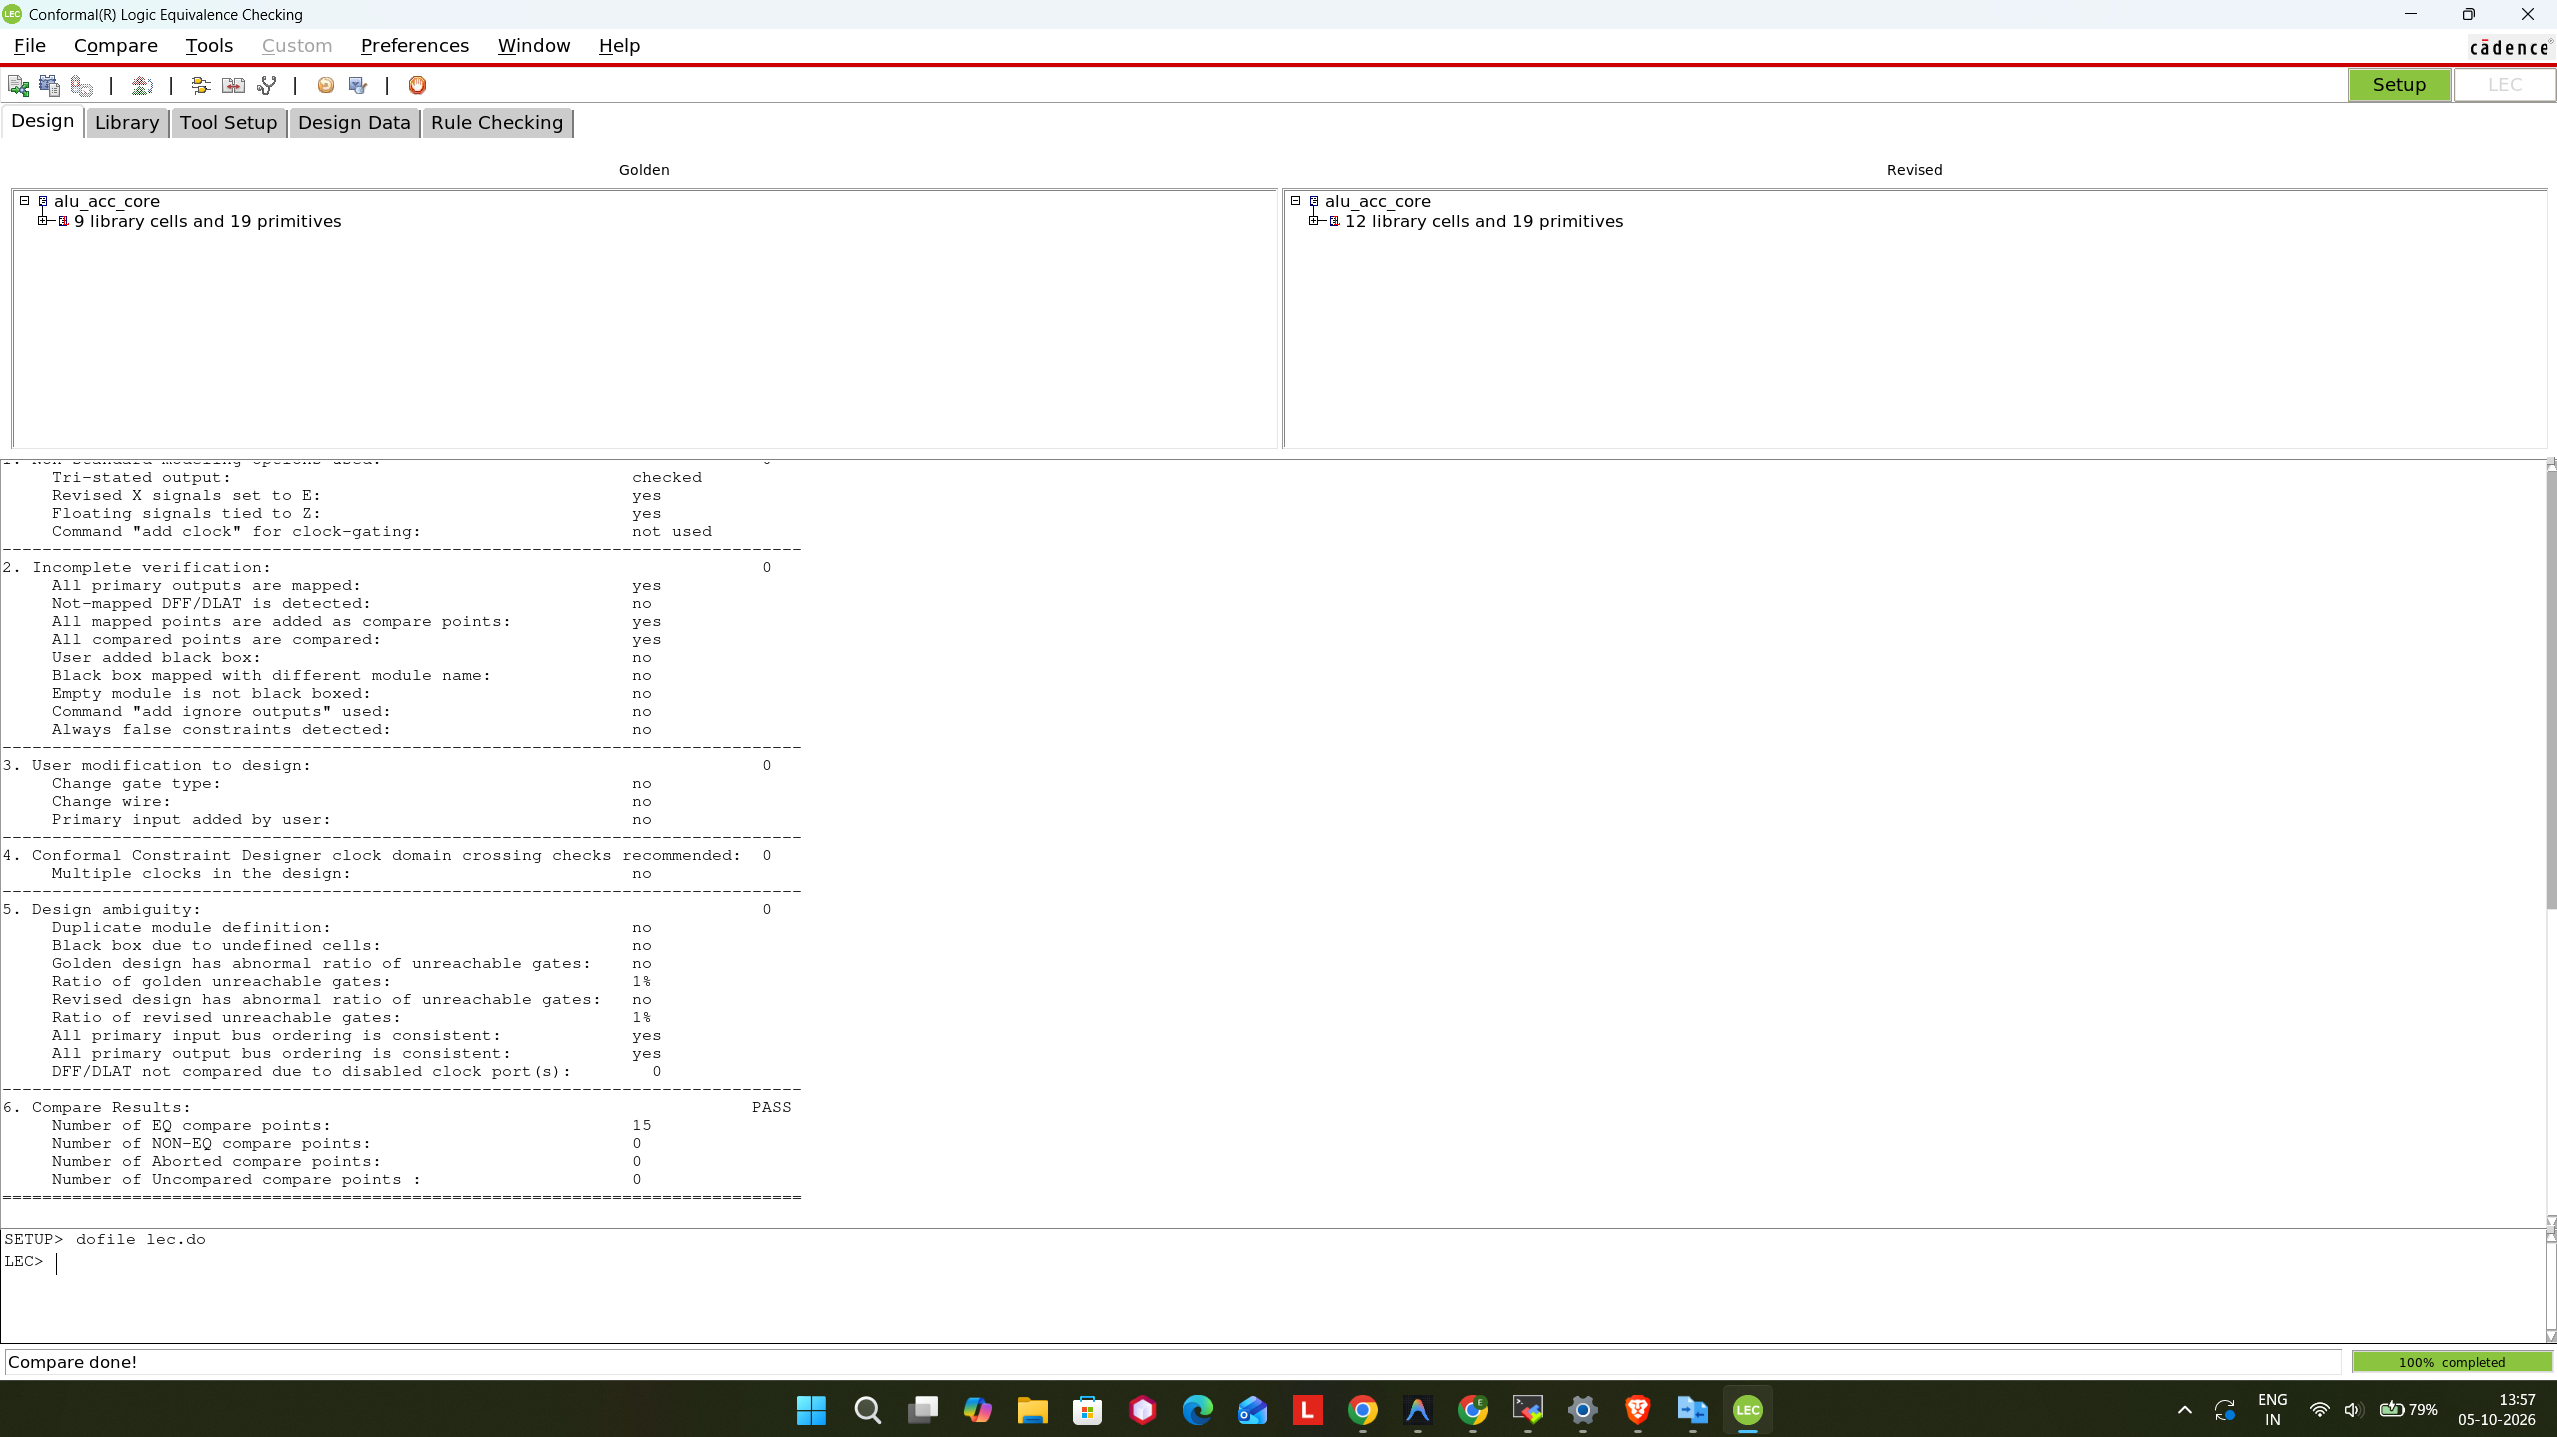
\includegraphics[width=0.8\textwidth]{Lab5_LEC_Exercises/Task4/output_task4_after_correction.png}
    \caption{Task 4 - PASS after correction}
\end{figure}


% --- TASK 5 ---
\section{Task 5: Hardcoded Reset Pin}
\textbf{Objective:} Debug an improperly constrained reset pin on a sequential element.

\textbf{Diagnosis:} 
Only a single flip-flop (\texttt{acc\_reg[2]}) failed. The schematic viewer showed that the \texttt{RN} (Active-Low Reset) pin was tied to a constant logic '1' instead of \texttt{rst\_n}.

\begin{figure}[H]
    \centering
    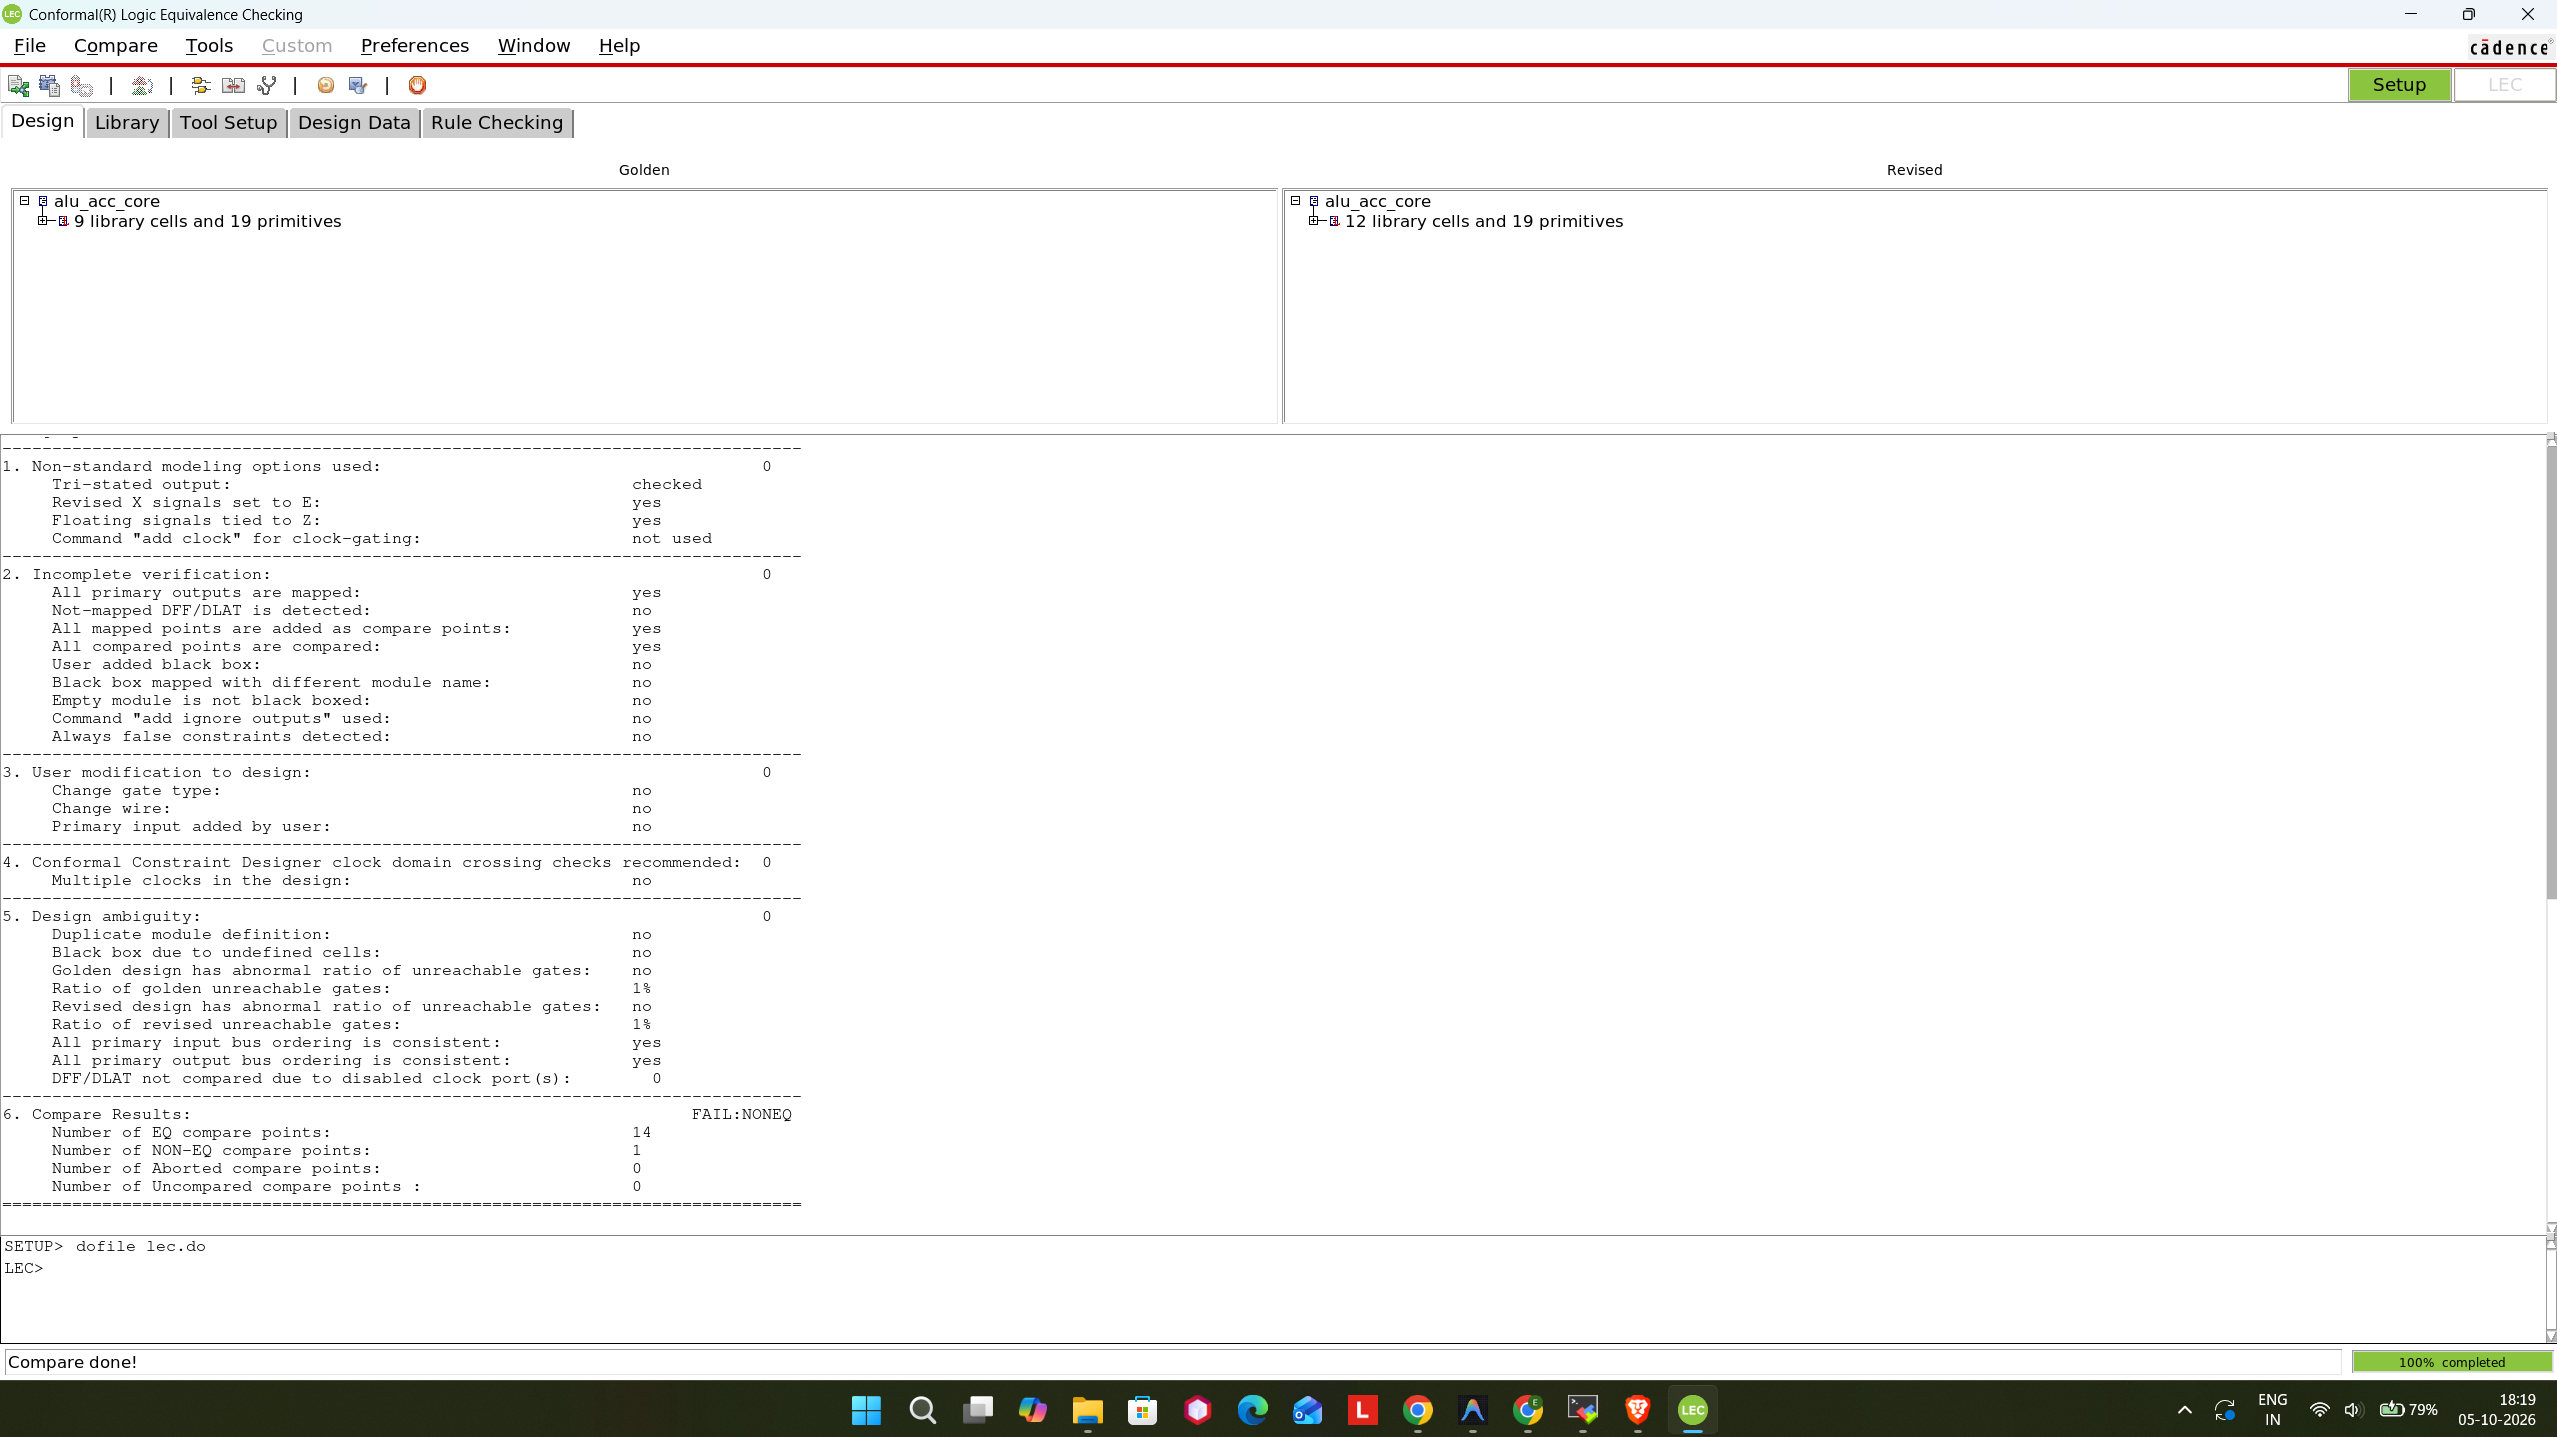
\includegraphics[width=0.8\textwidth]{Lab5_LEC_Exercises/Task5/output_task5.png}
    \caption{Task 5 - Initial Failure}
\end{figure}
\begin{figure}[H]
    \centering
    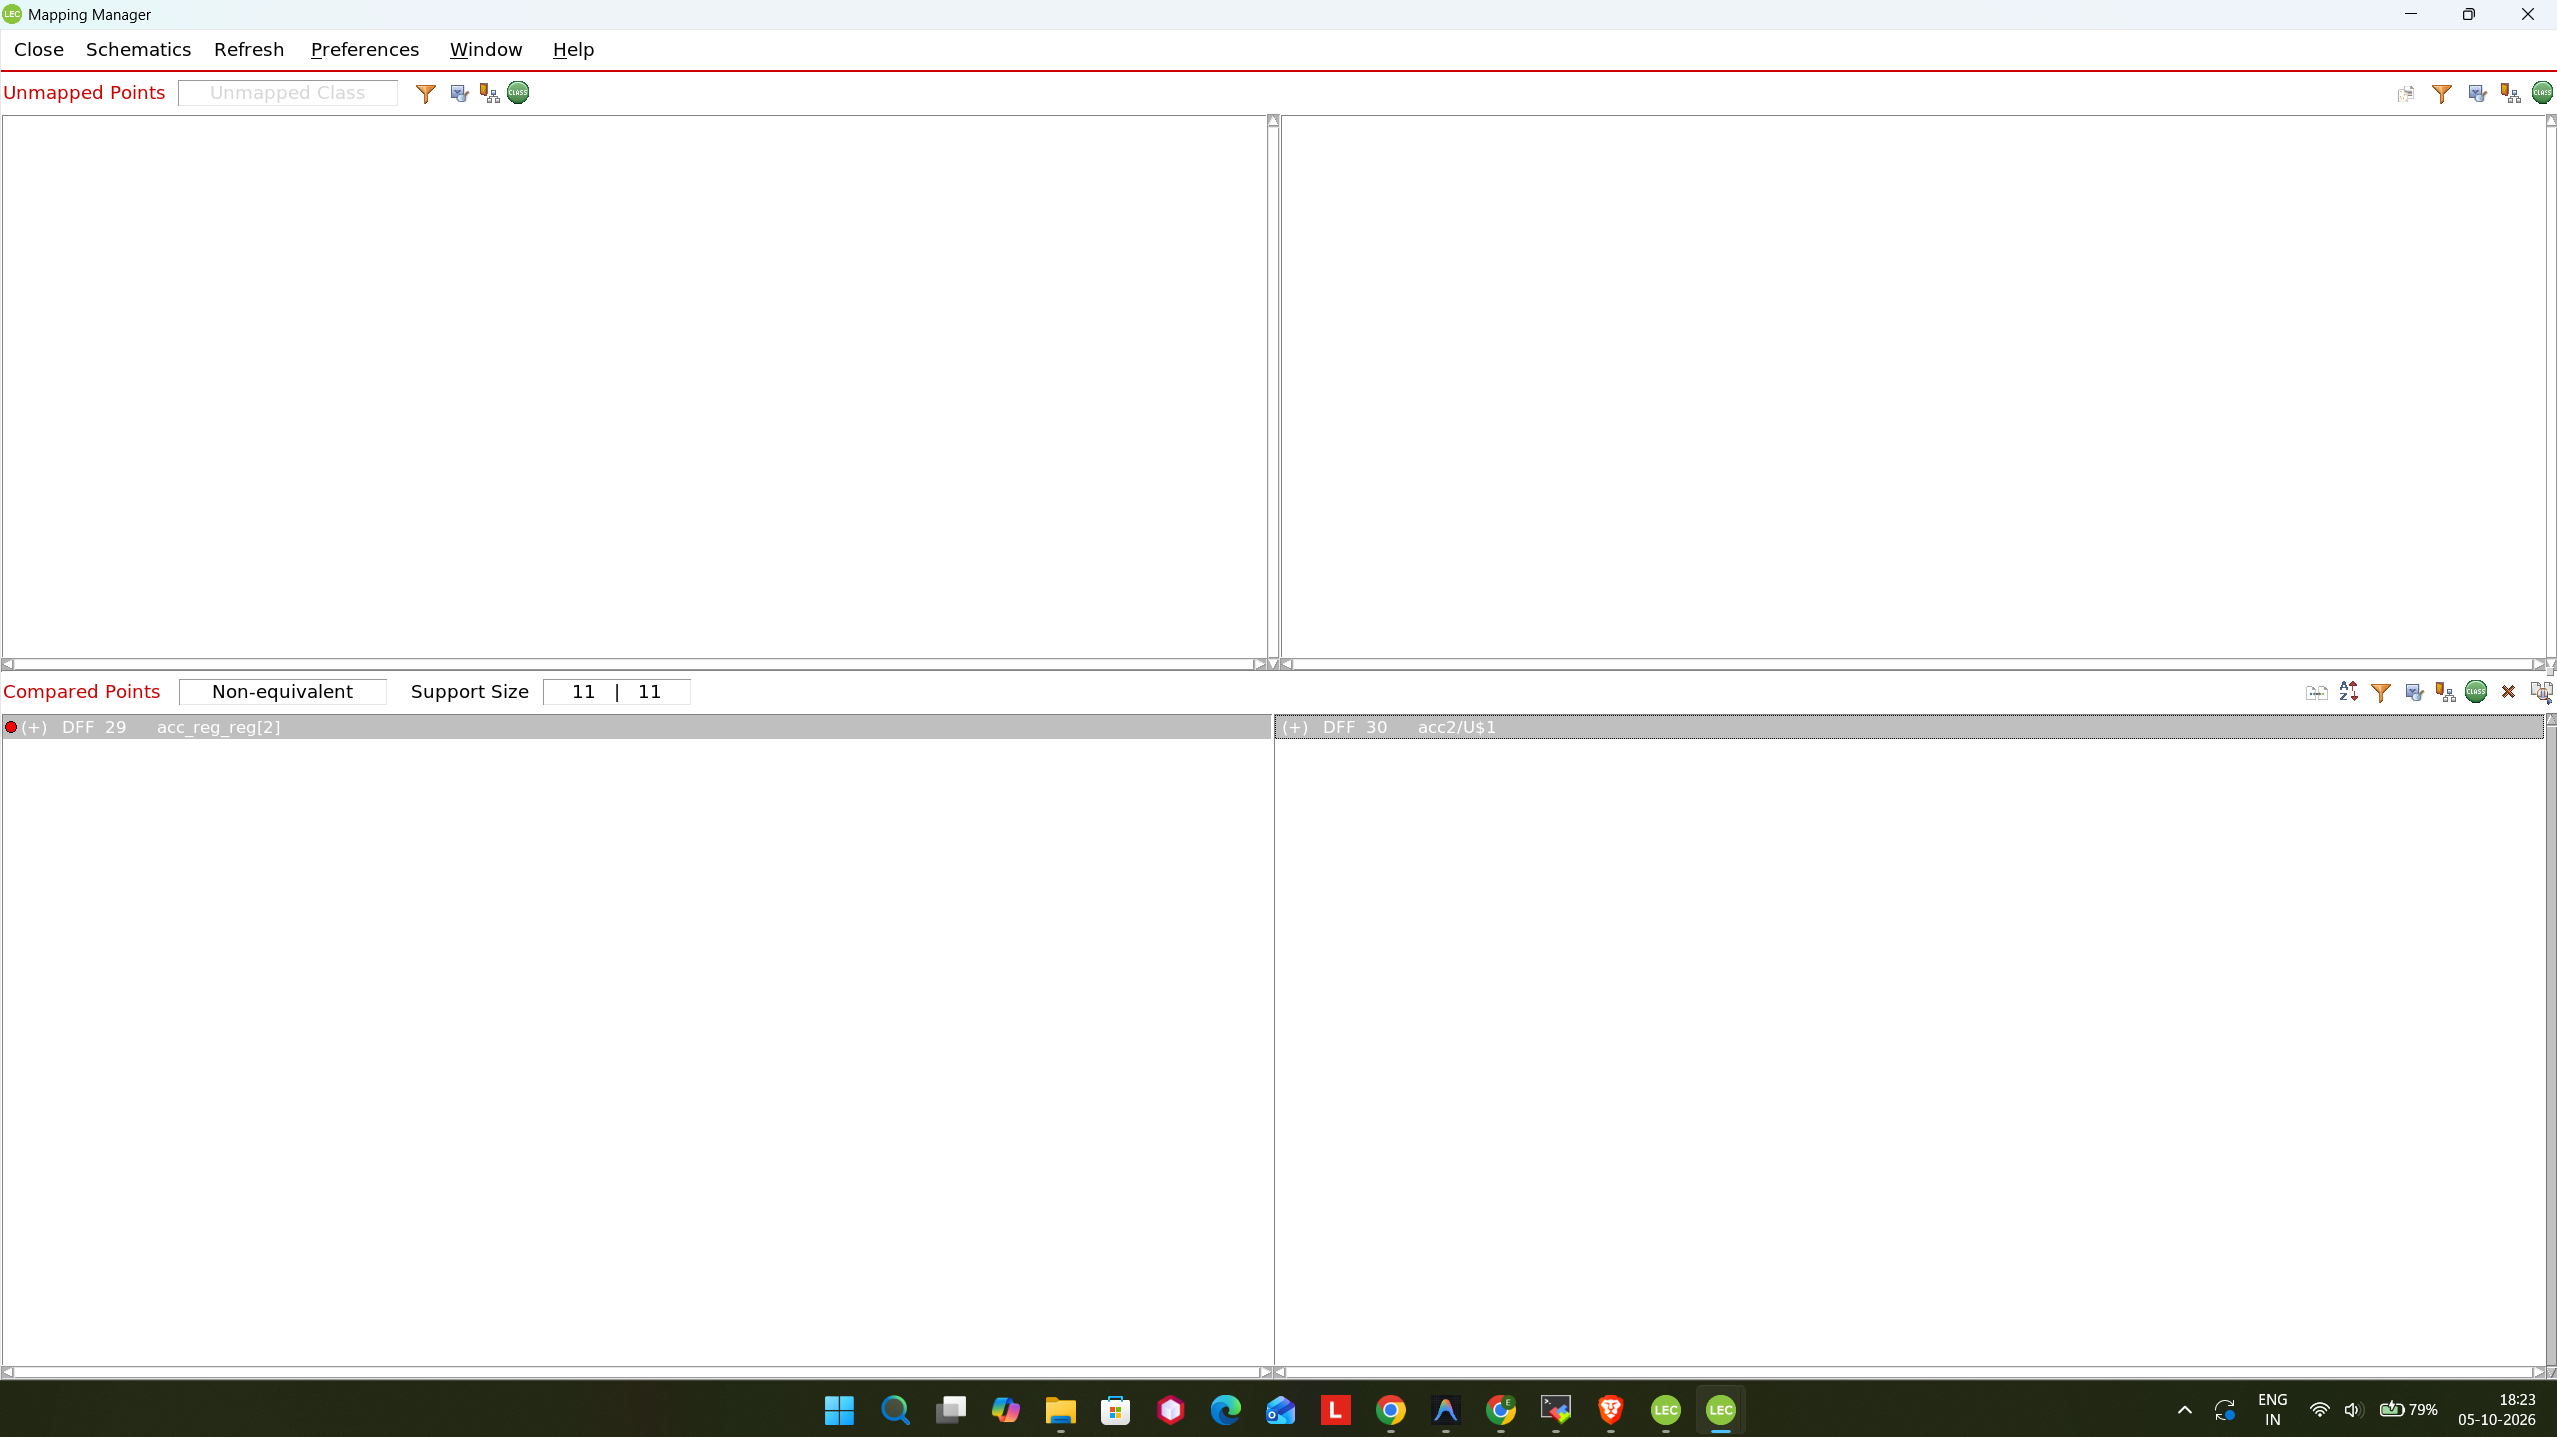
\includegraphics[width=0.8\textwidth]{Lab5_LEC_Exercises/Task5/mapping_magaer_task5.png}
    \caption{Task 5 - Mapping Manager isolating the single DFF}
\end{figure}
\begin{figure}[H]
    \centering
    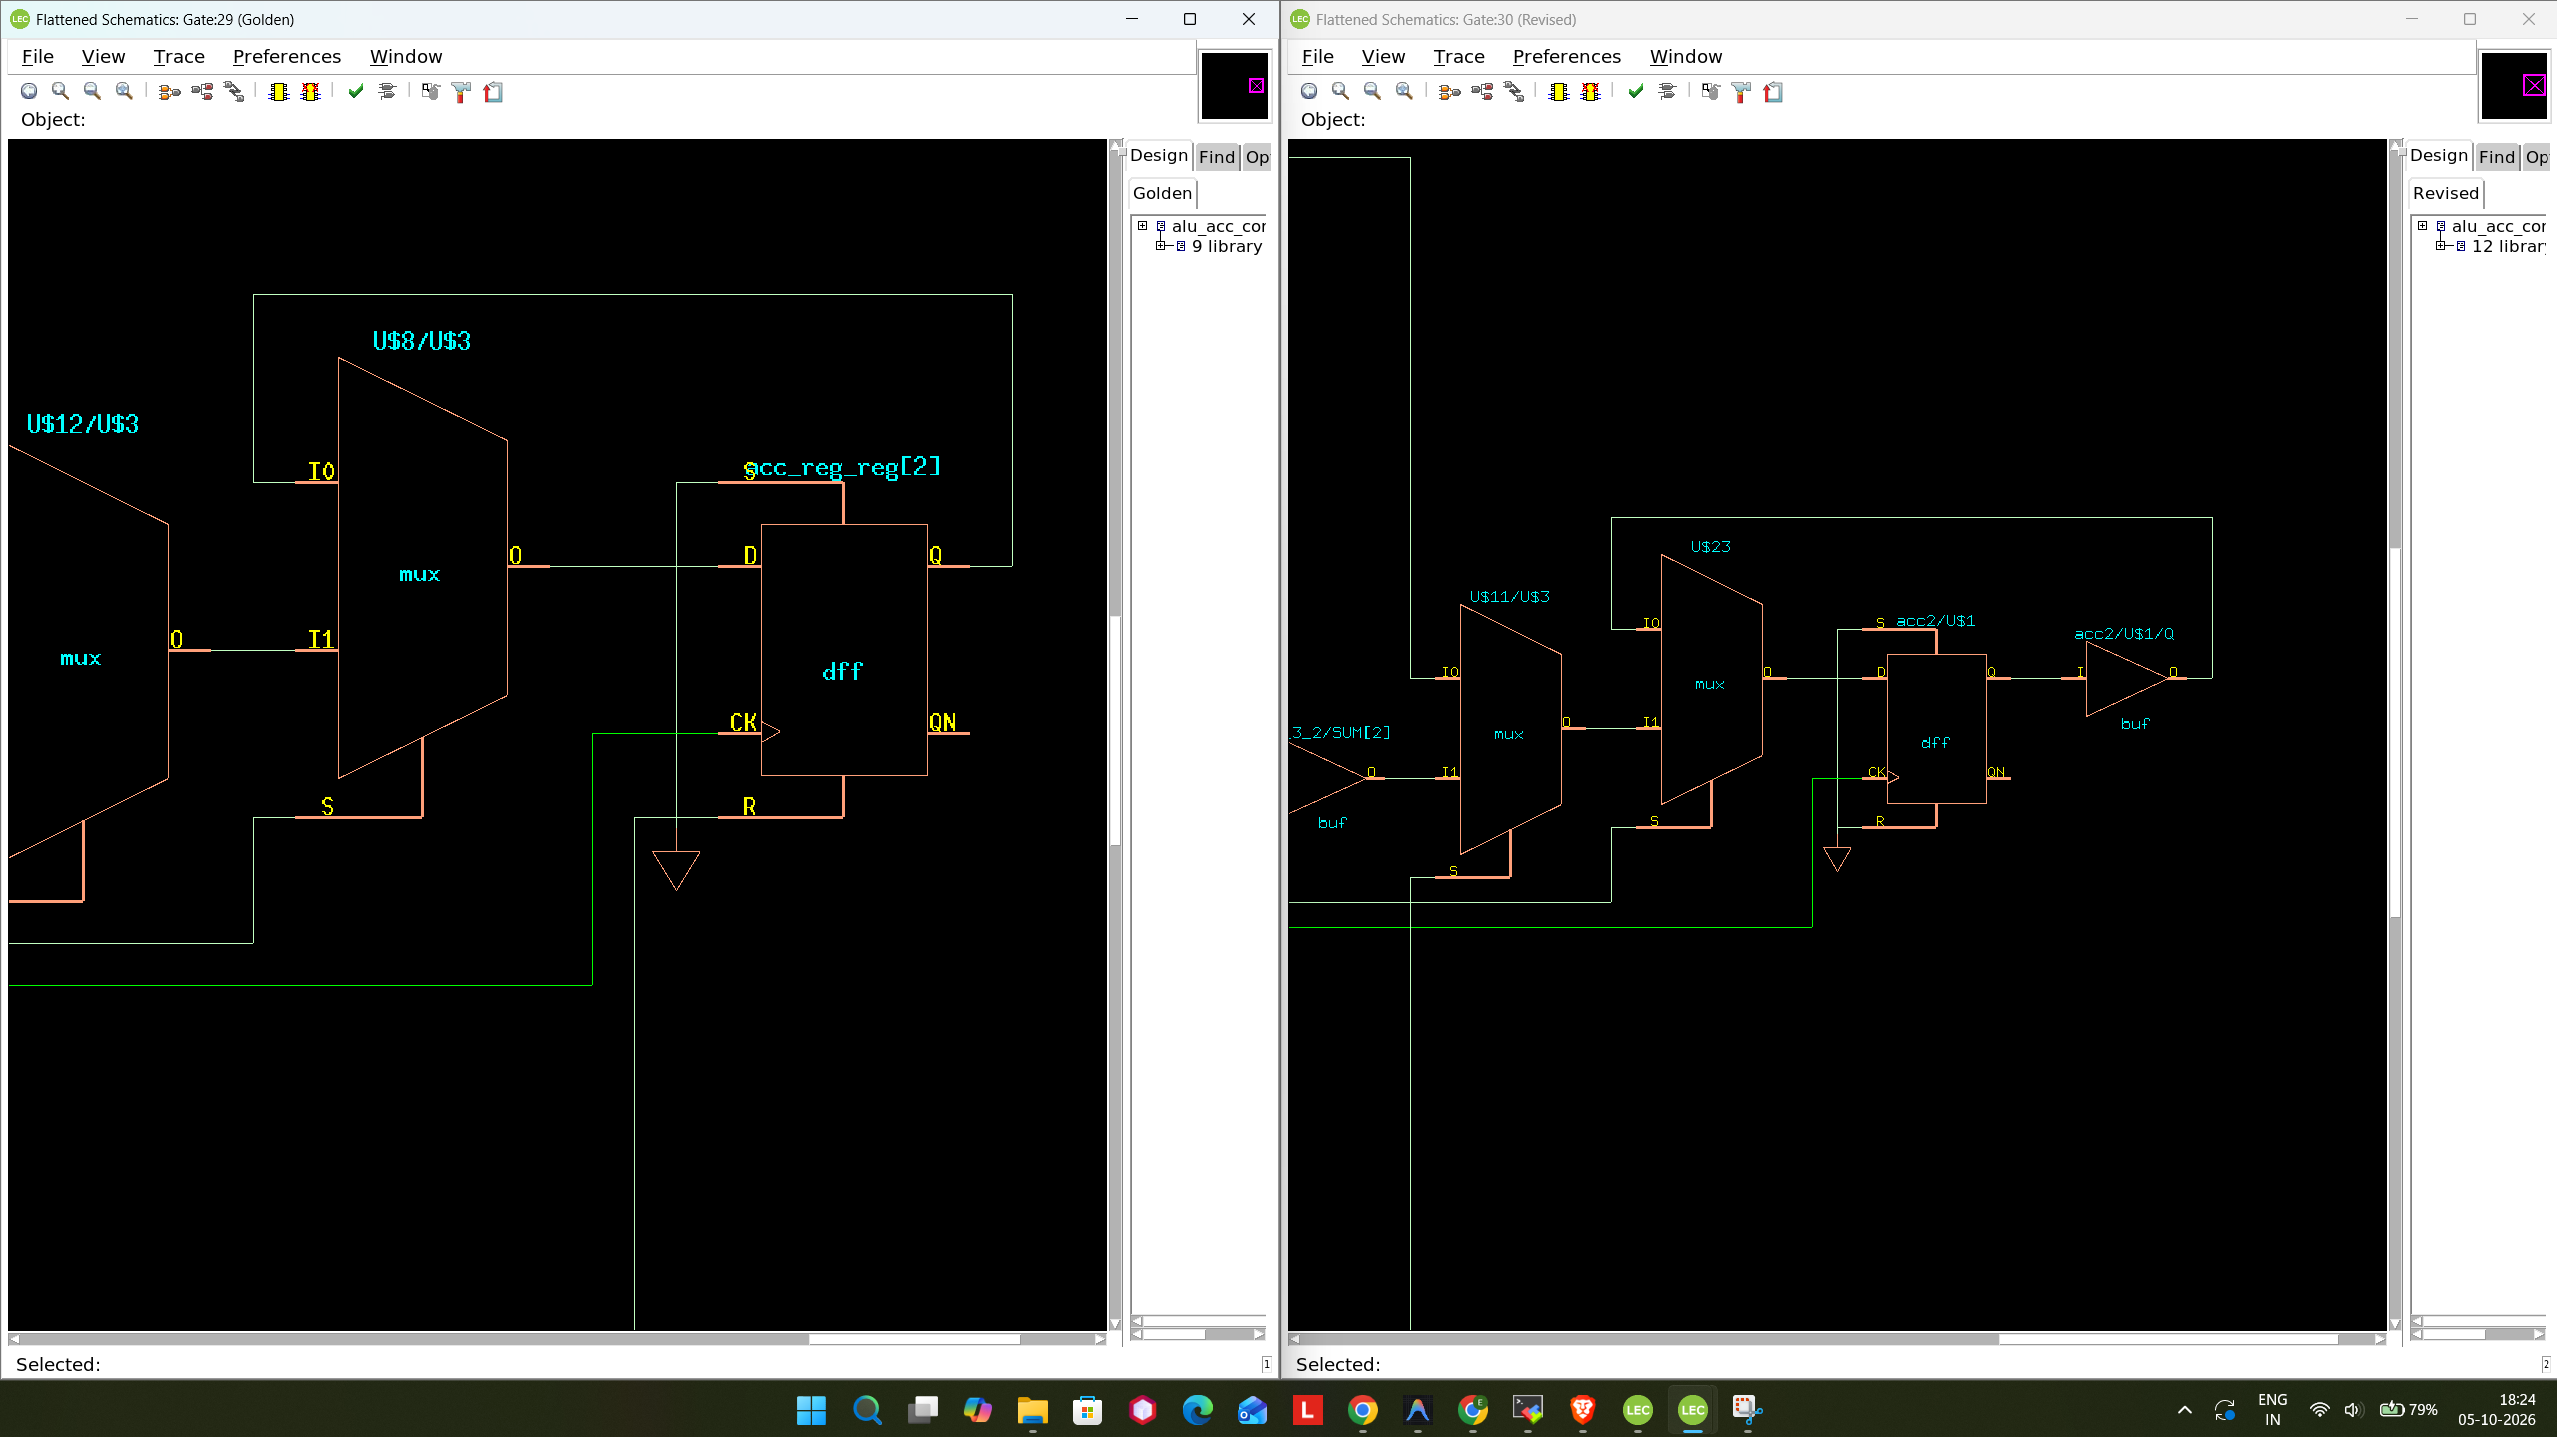
\includegraphics[width=0.8\textwidth]{Lab5_LEC_Exercises/Task5/schematics_task5.png}
    \caption{Task 5 - Schematic showing hardcoded reset pin (Logic 1)}
\end{figure}

\textbf{Correction:} 
The pin connection was restored to the \texttt{rst\_n} net.
\begin{lstlisting}[language=Verilog]
// Original Broken Code:
DFFRX1 acc2(.D(en?result[2]:acc_reg[2]),.RN(1'b1),.CK(clk),.Q(acc_reg[2]));

// Corrected Code:
DFFRX1 acc2(.D(en?result[2]:acc_reg[2]),.RN(rst_n),.CK(clk),.Q(acc_reg[2]));
\end{lstlisting}

\begin{figure}[H]
    \centering
    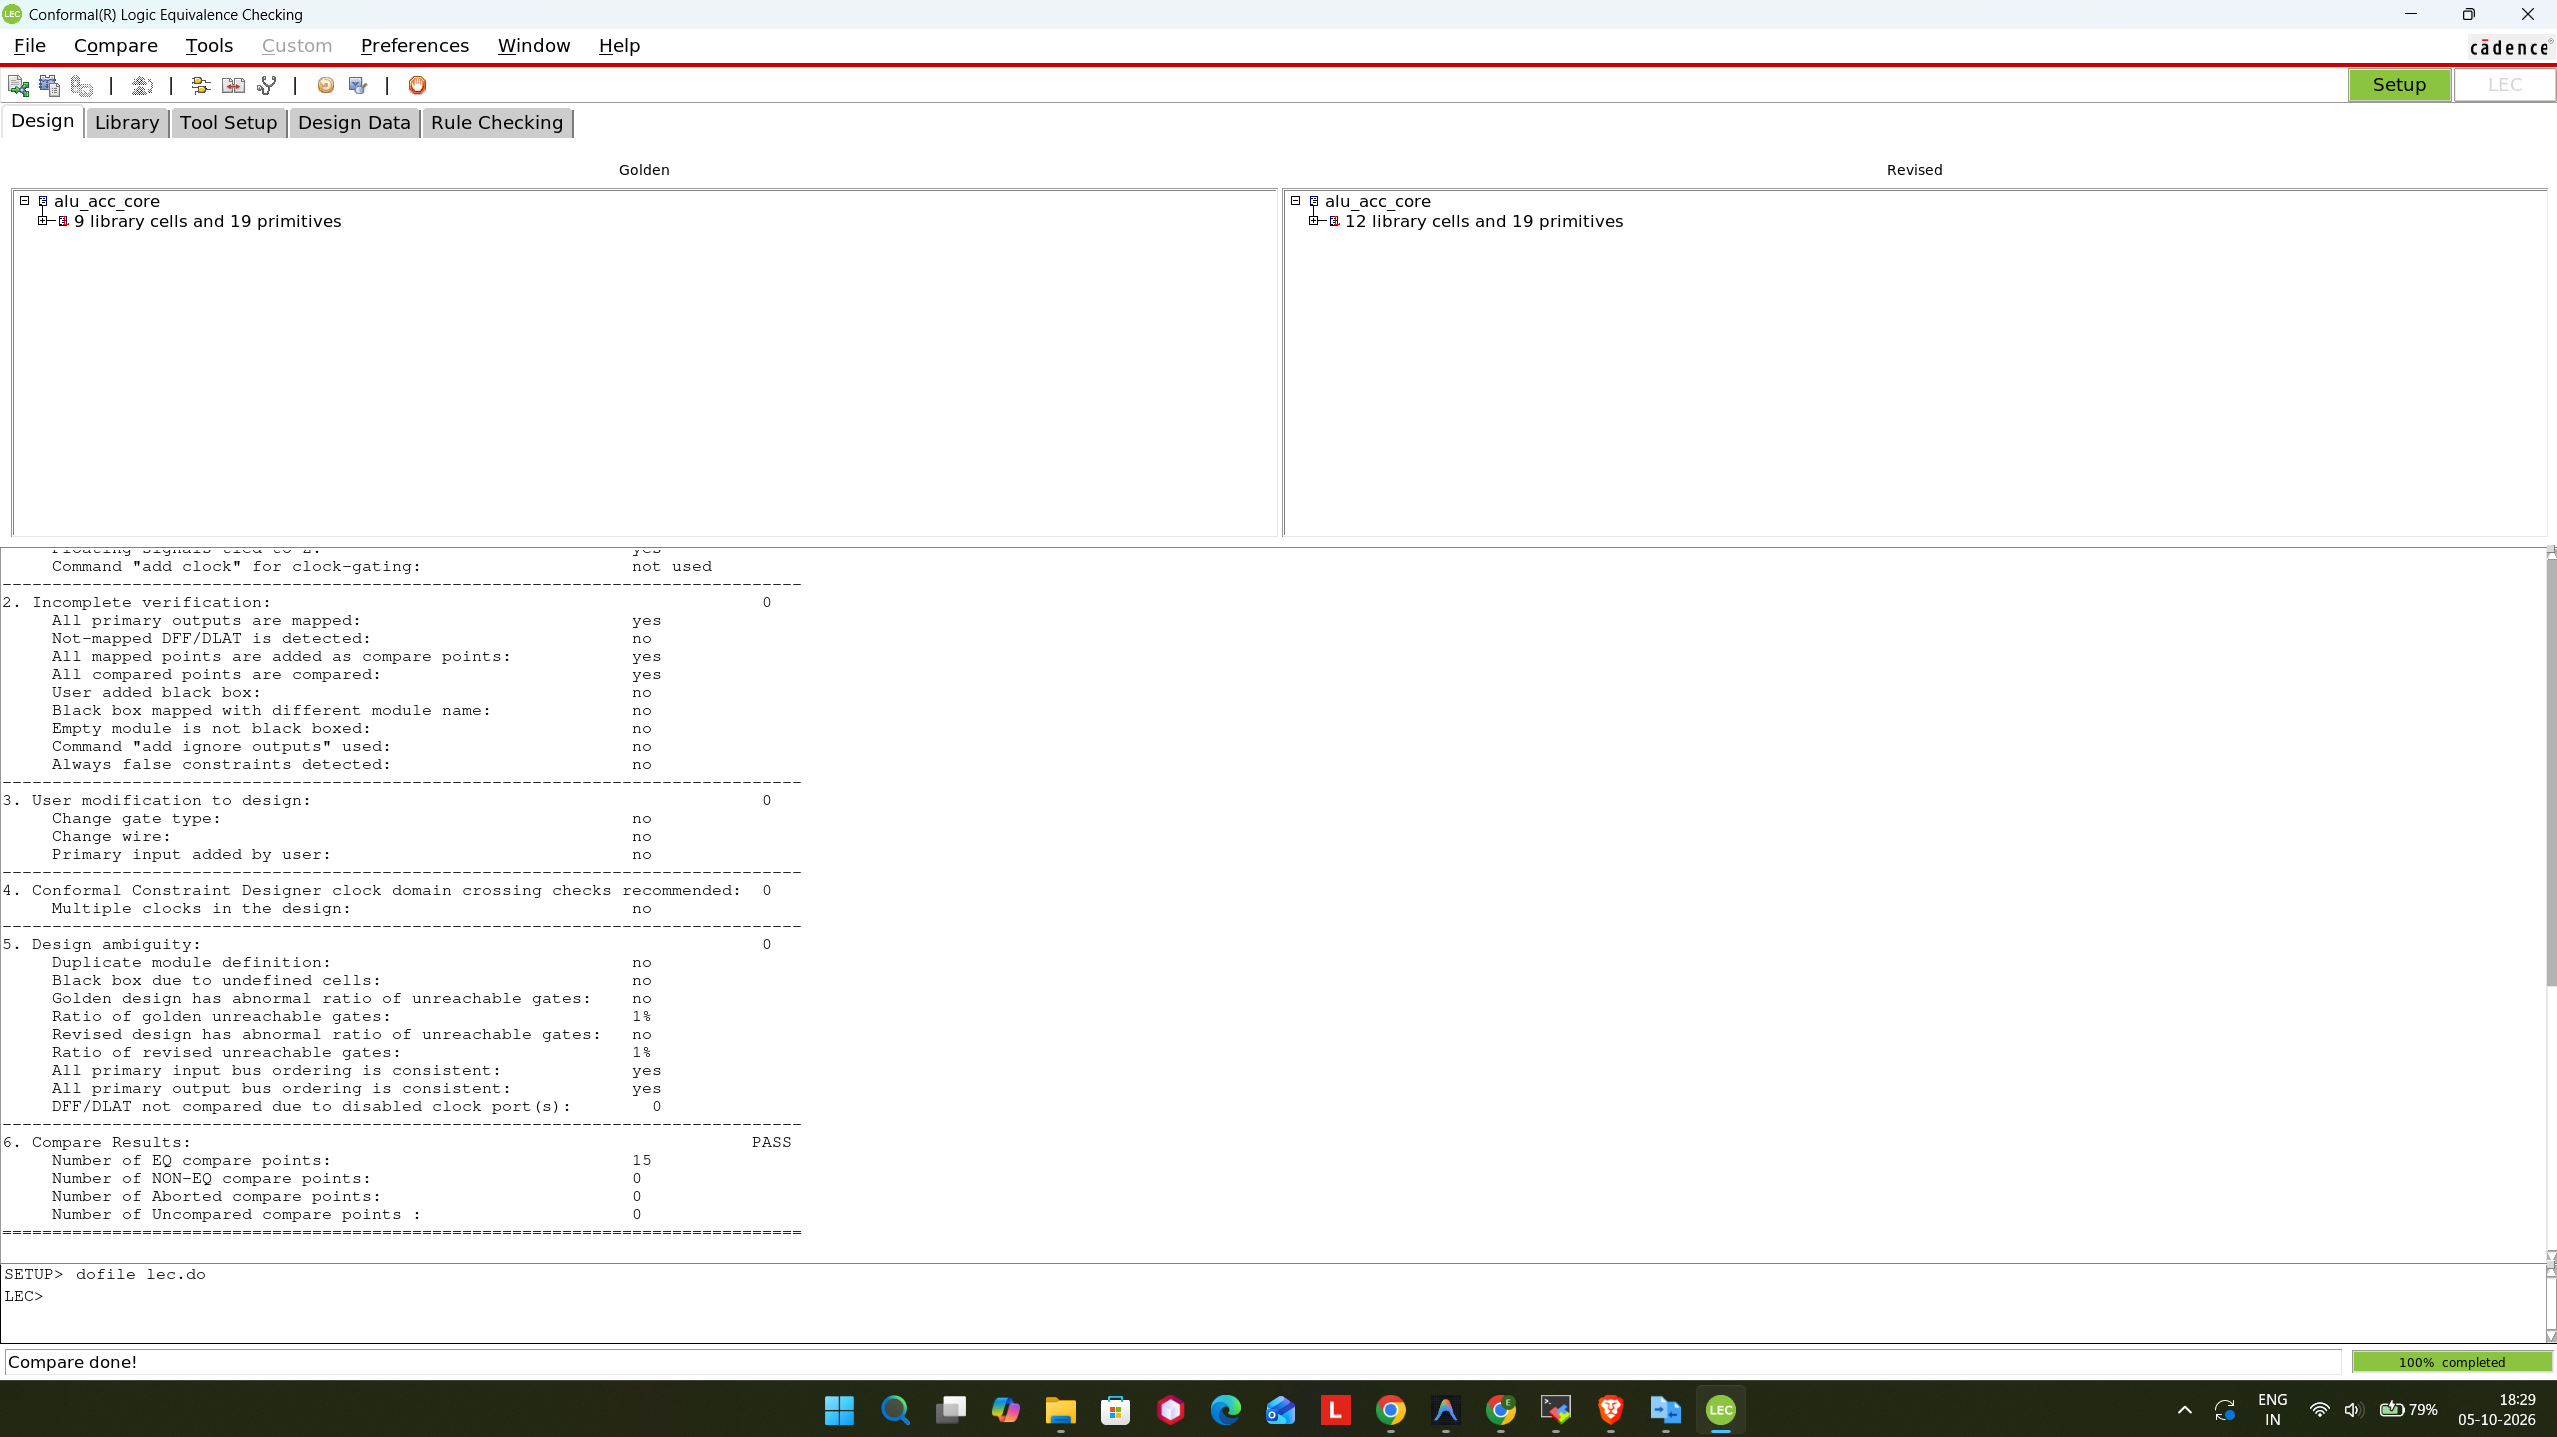
\includegraphics[width=0.8\textwidth]{Lab5_LEC_Exercises/Task5/output_after_correction_task5.png}
    \caption{Task 5 - PASS after correction}
\end{figure}


% --- TASK 6 ---
\section{Task 6: Incorrect Primary Output Wiring}
\textbf{Objective:} Fix a primary output that was wired to the wrong input source.

\textbf{Diagnosis:} 
The \texttt{test\_status} primary output failed. In the Golden design, this pin is hardwired to logic 0. In the Revised design, it was accidentally connected to the \texttt{test\_mode} input pin.

\begin{figure}[H]
    \centering
    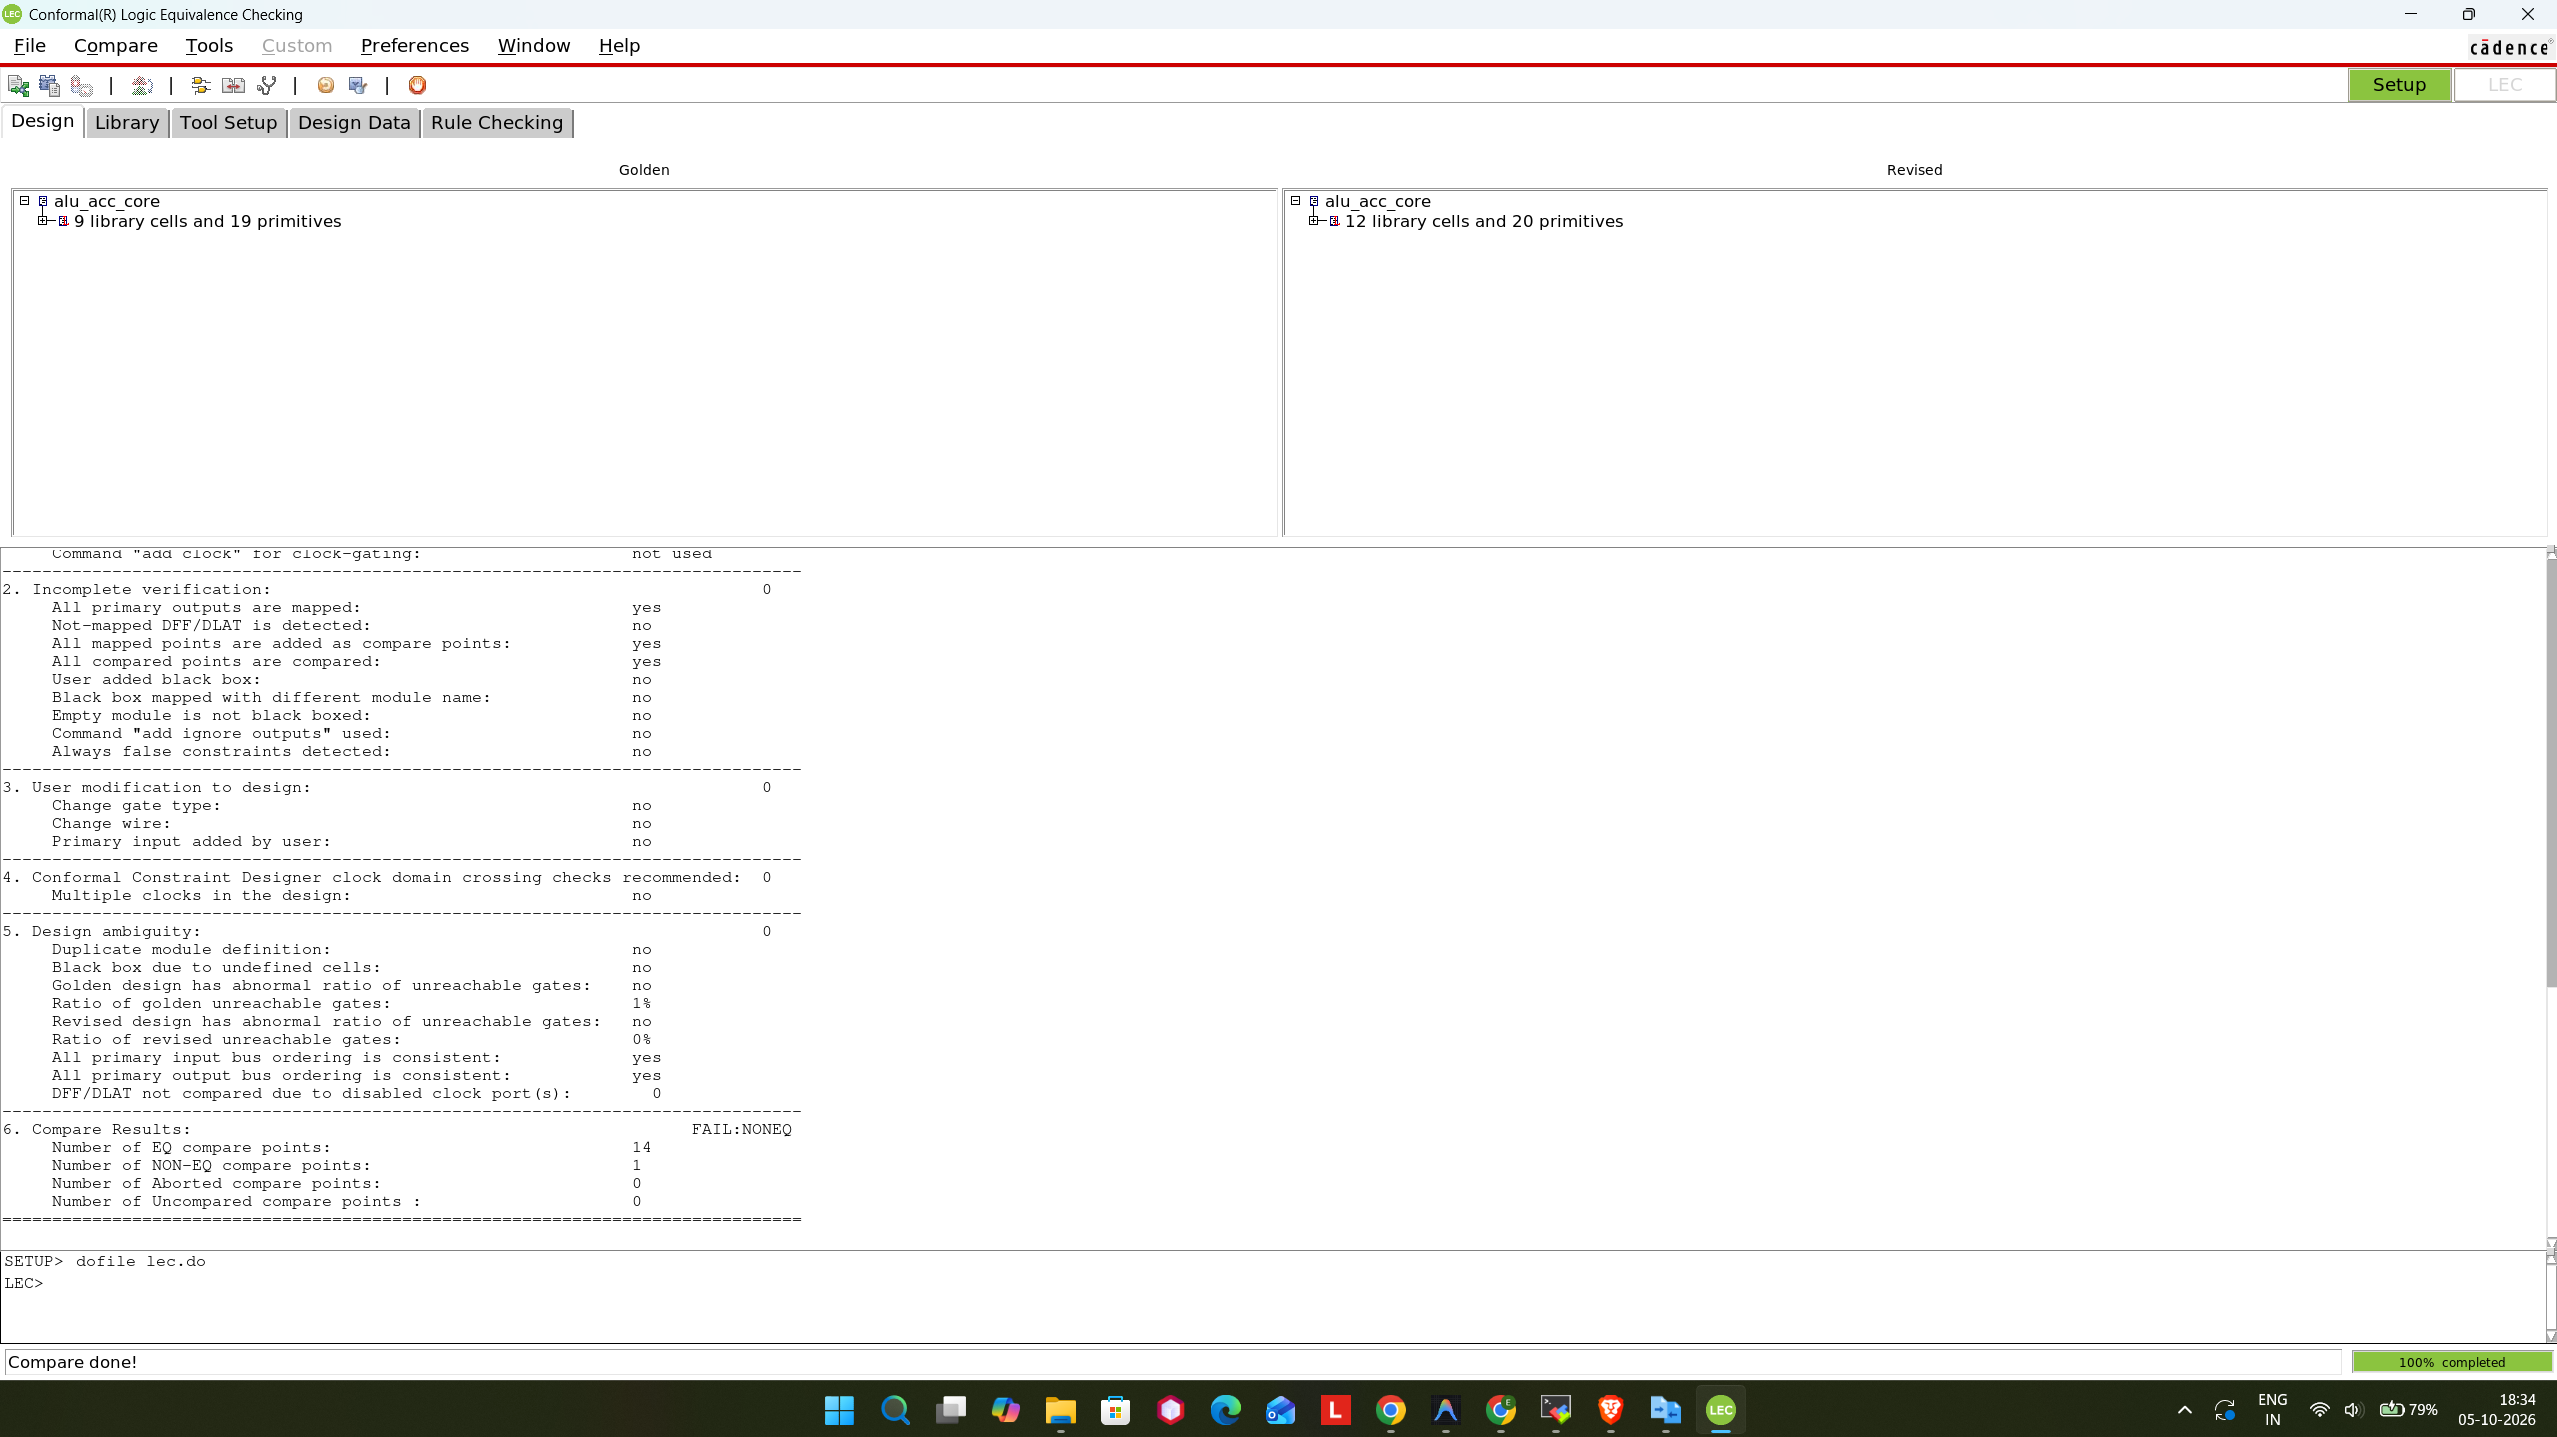
\includegraphics[width=0.8\textwidth]{Lab5_LEC_Exercises/Task6/output_task6.png}
    \caption{Task 6 - Initial Failure}
\end{figure}
\begin{figure}[H]
    \centering
    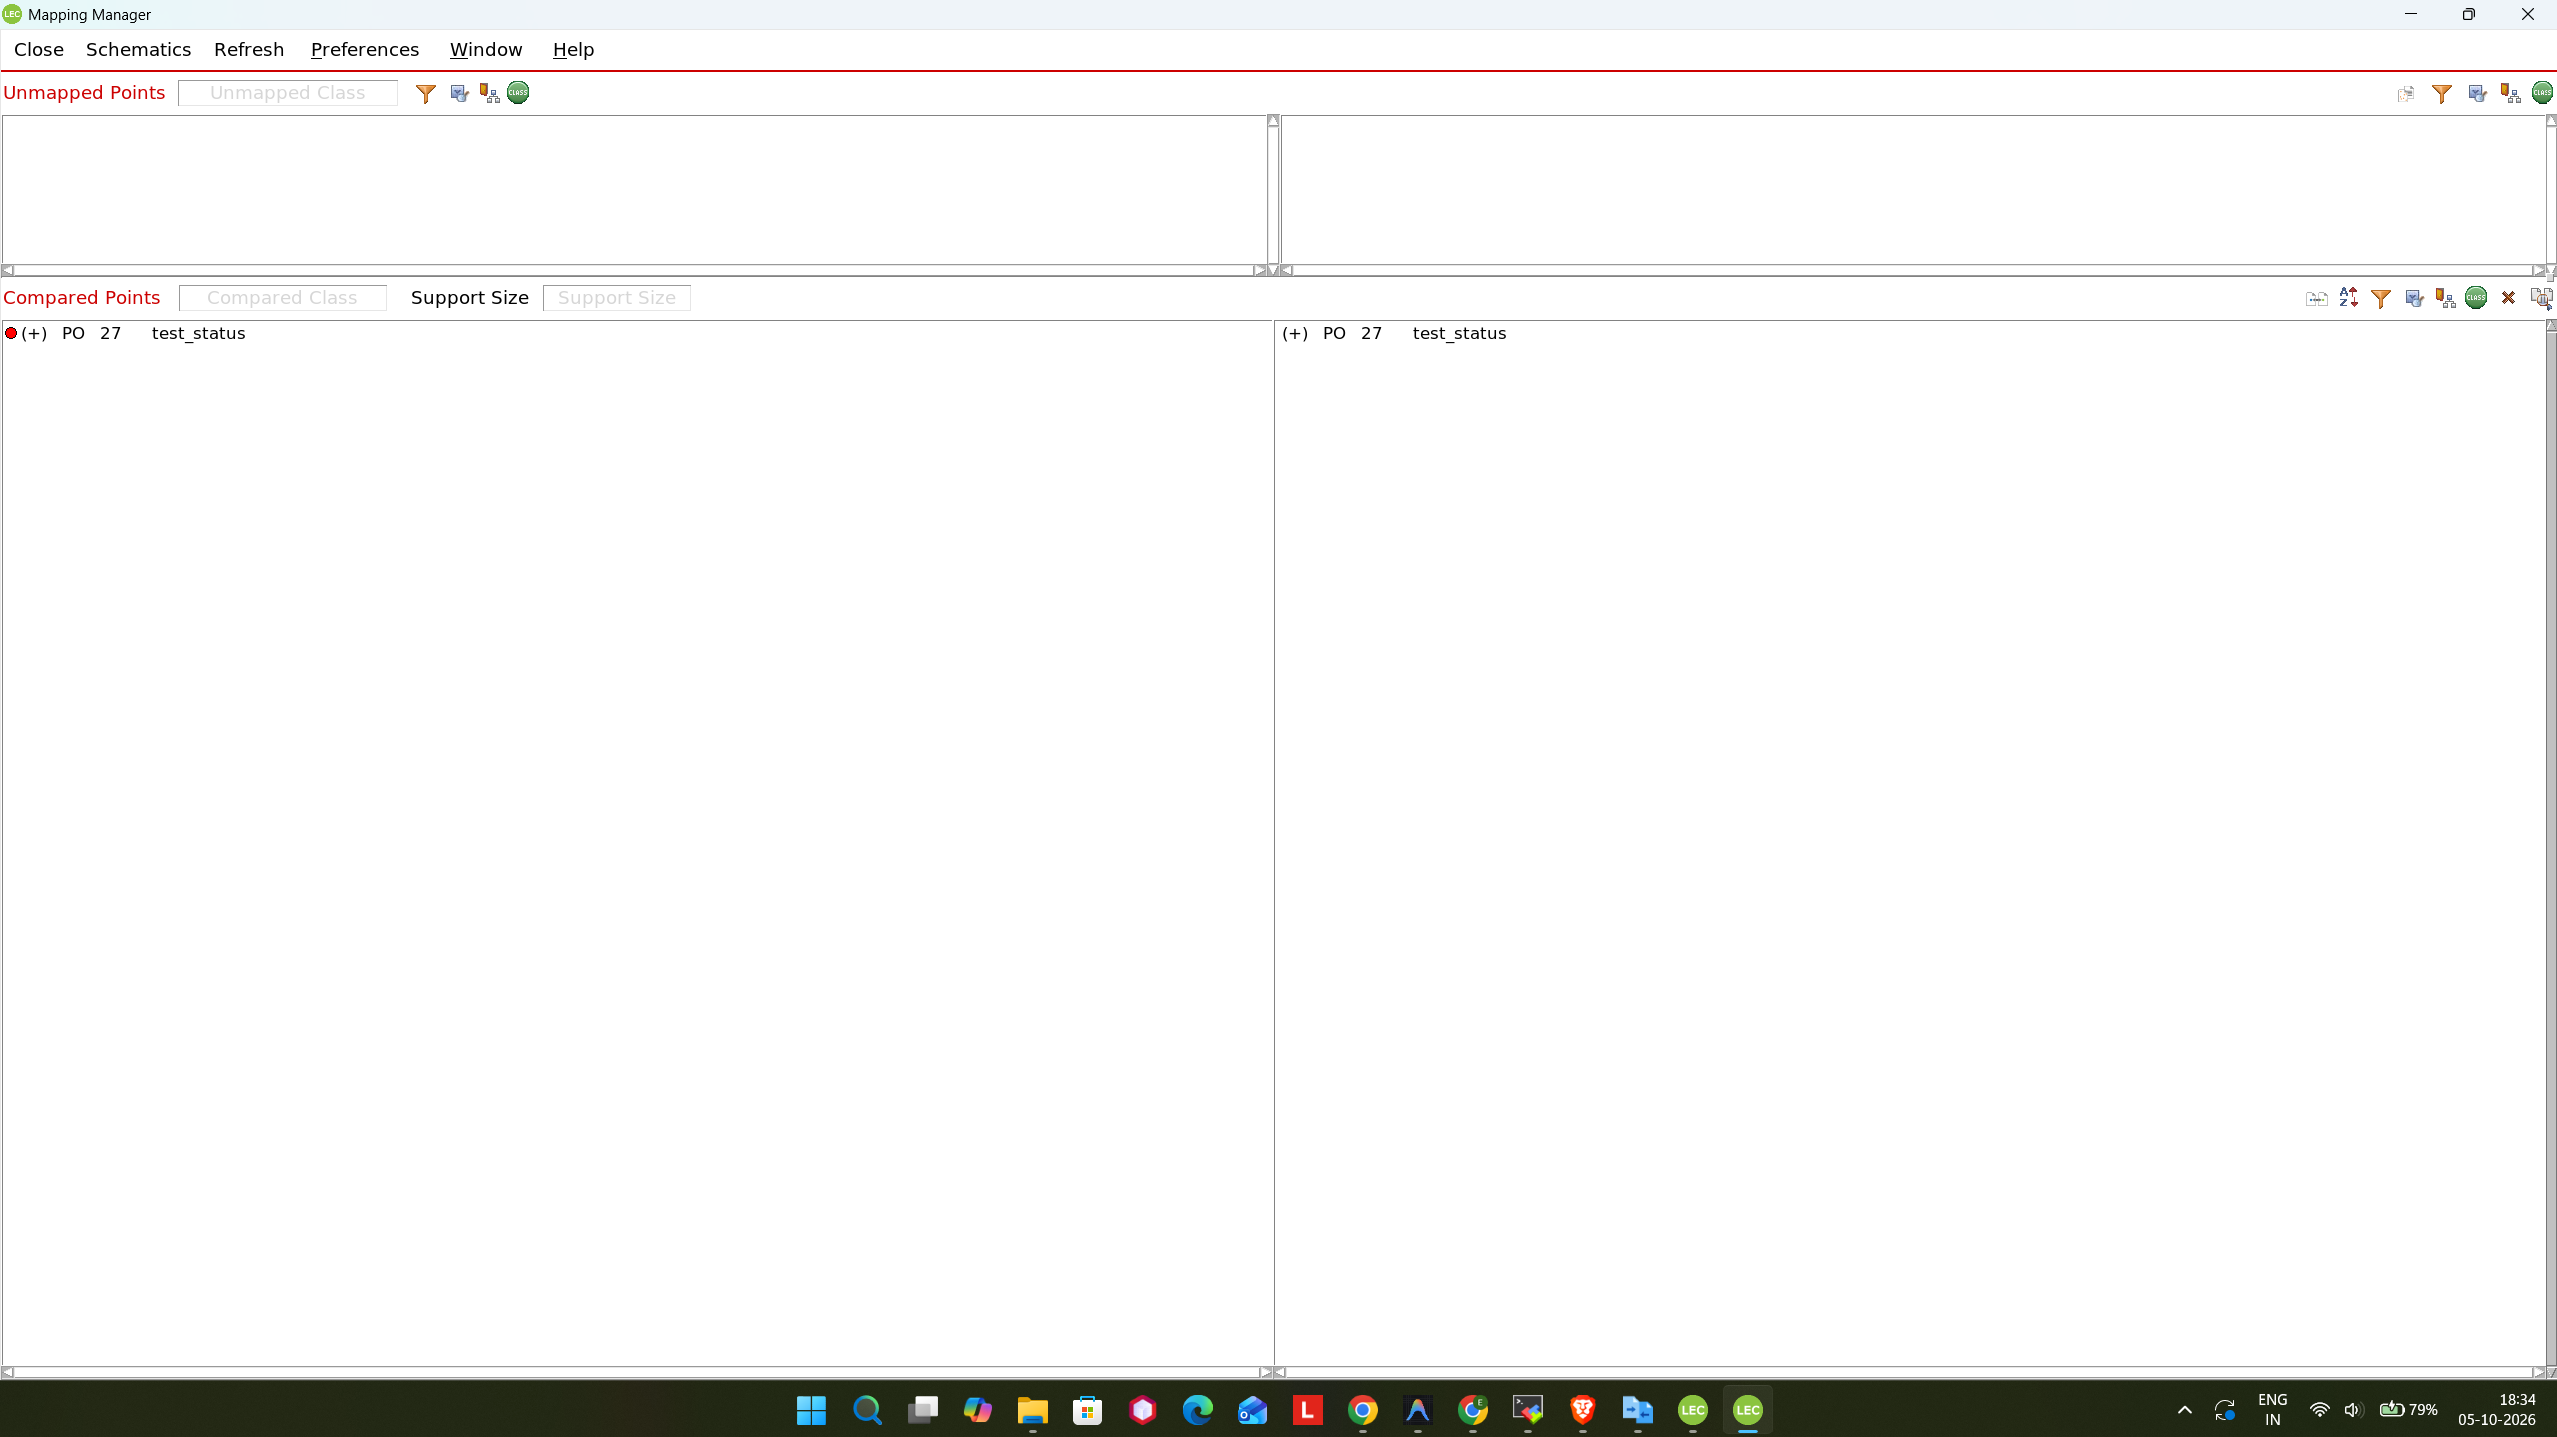
\includegraphics[width=0.8\textwidth]{Lab5_LEC_Exercises/Task6/mapping_manager_task6.png}
    \caption{Task 6 - Mapping Manager pointing to test\_status}
\end{figure}
\begin{figure}[H]
    \centering
    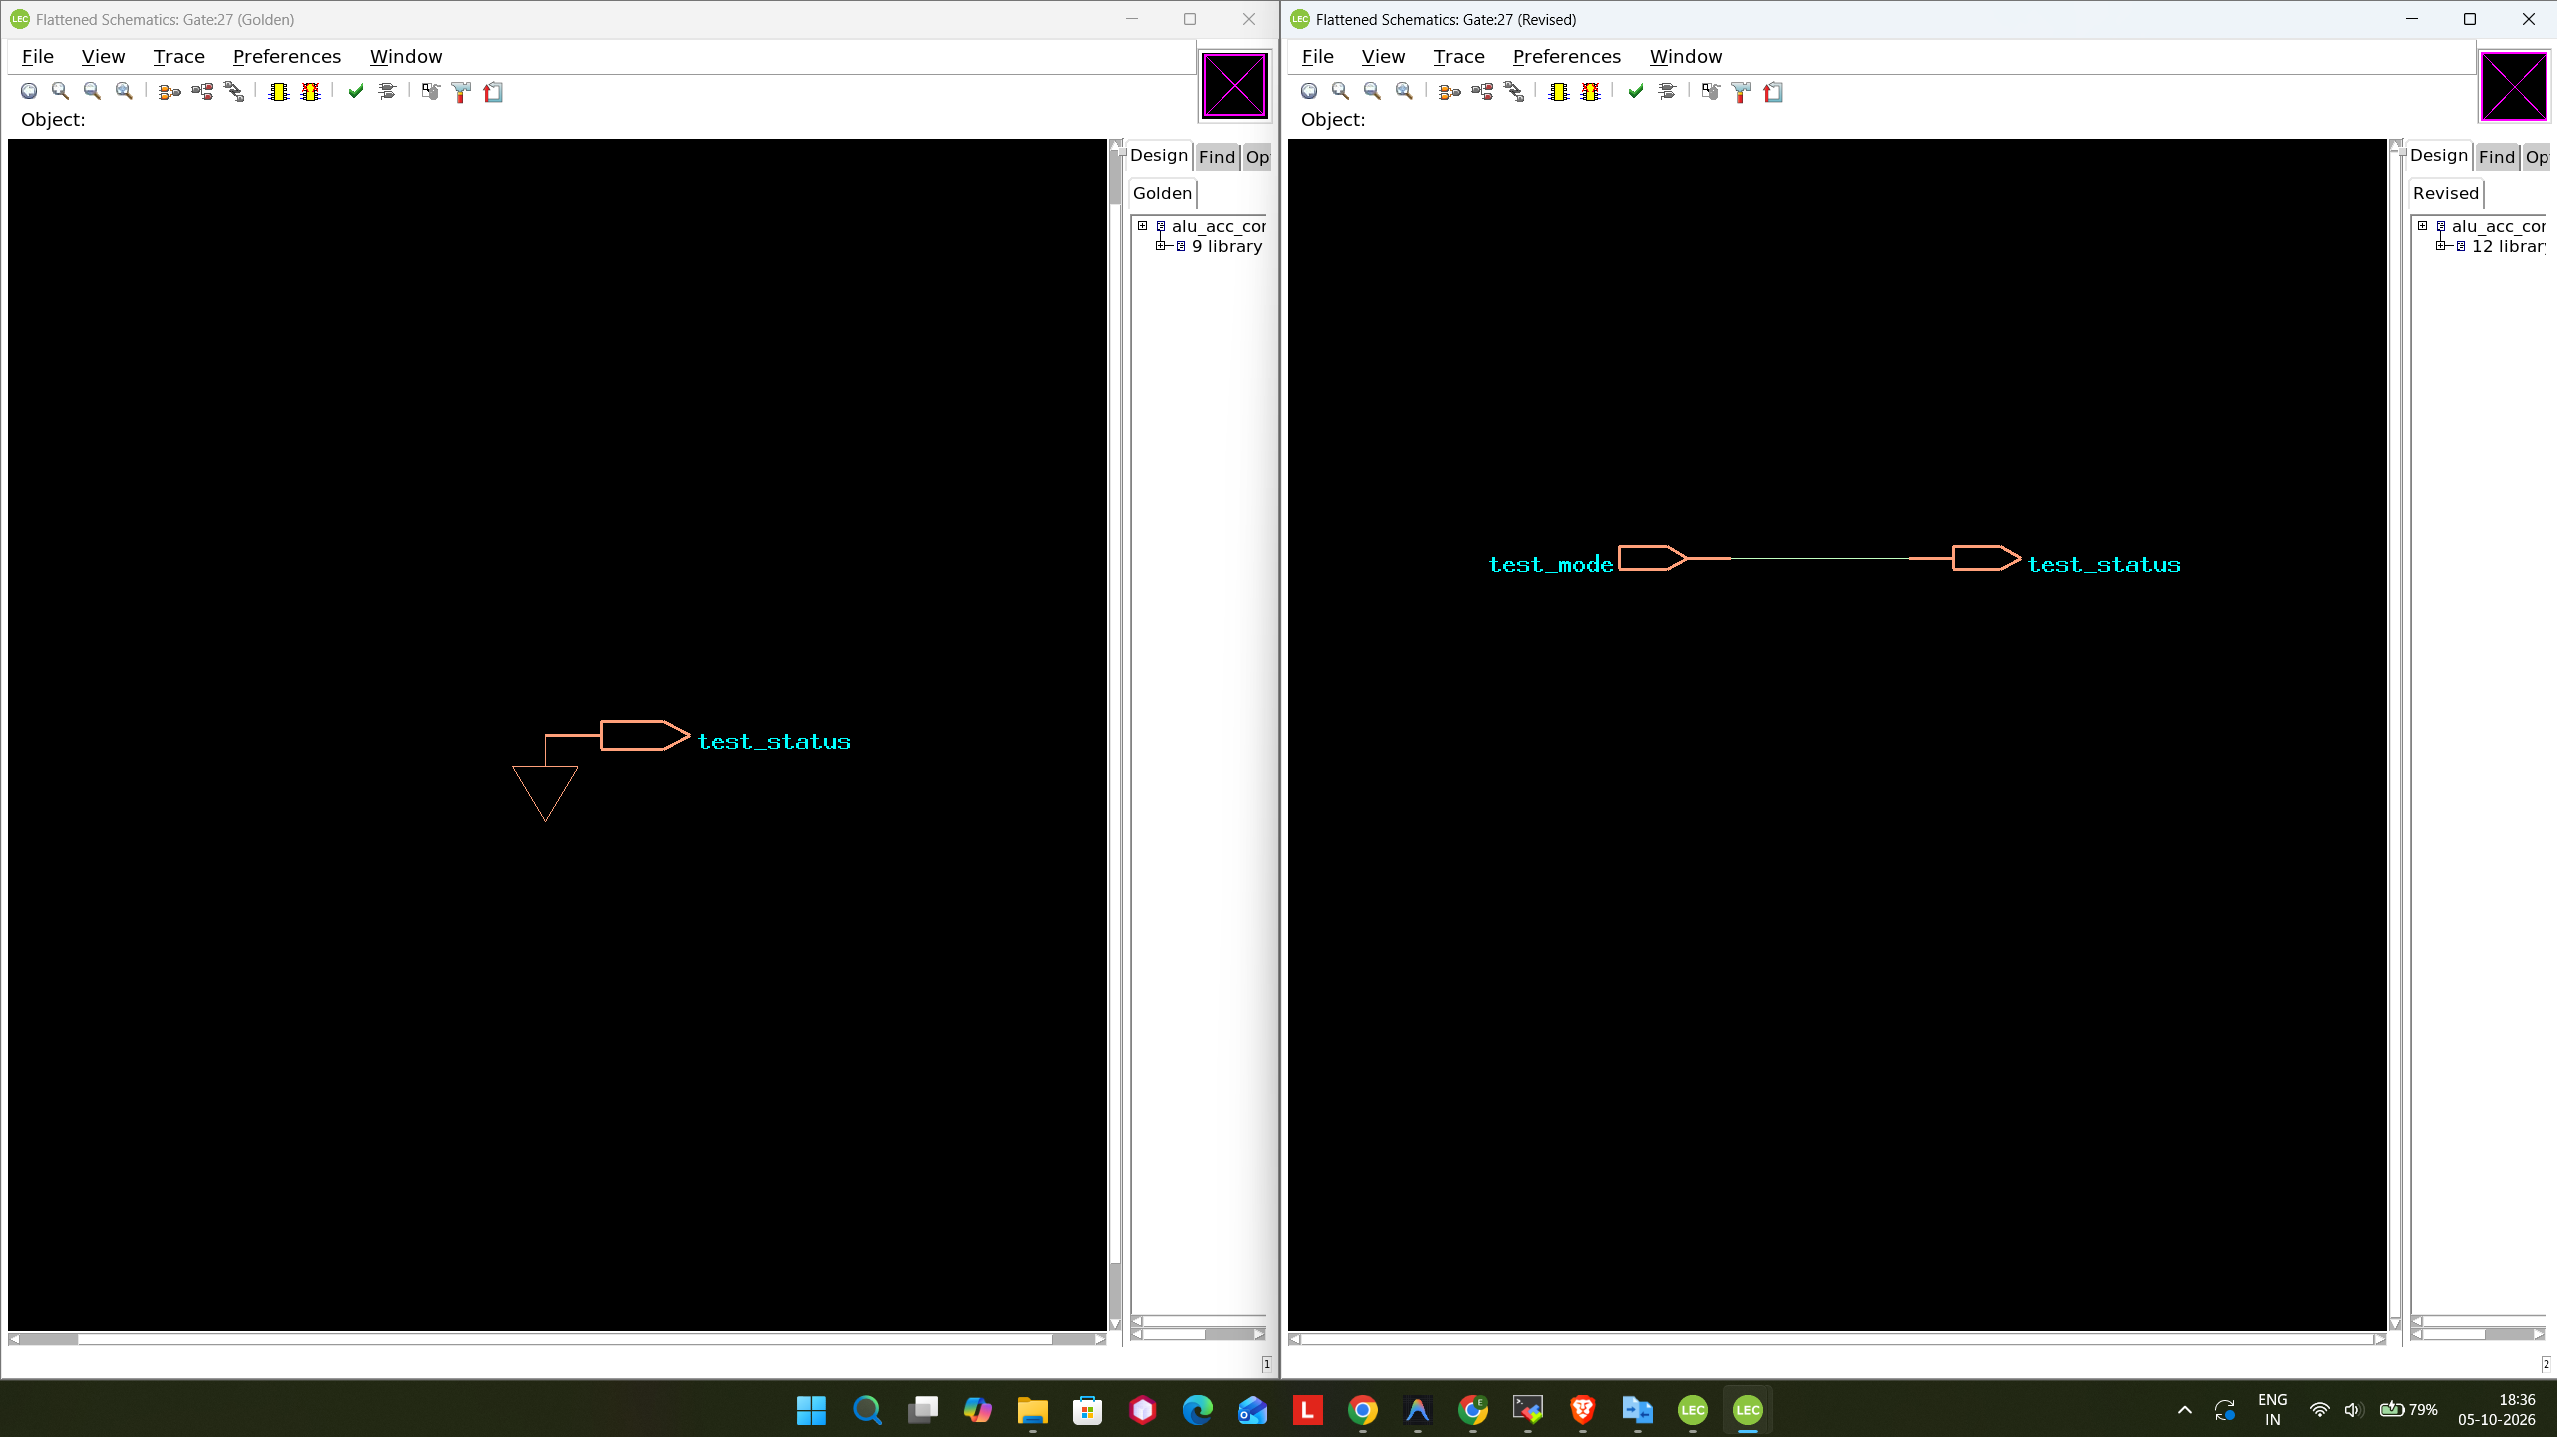
\includegraphics[width=0.8\textwidth]{Lab5_LEC_Exercises/Task6/schematics_task6.png}
    \caption{Task 6 - Schematic showing bad wiring}
\end{figure}

\textbf{Correction:} 
\begin{lstlisting}[language=Verilog]
// Corrected Code:
assign test_status=1'b0;
\end{lstlisting}

\begin{figure}[H]
    \centering
    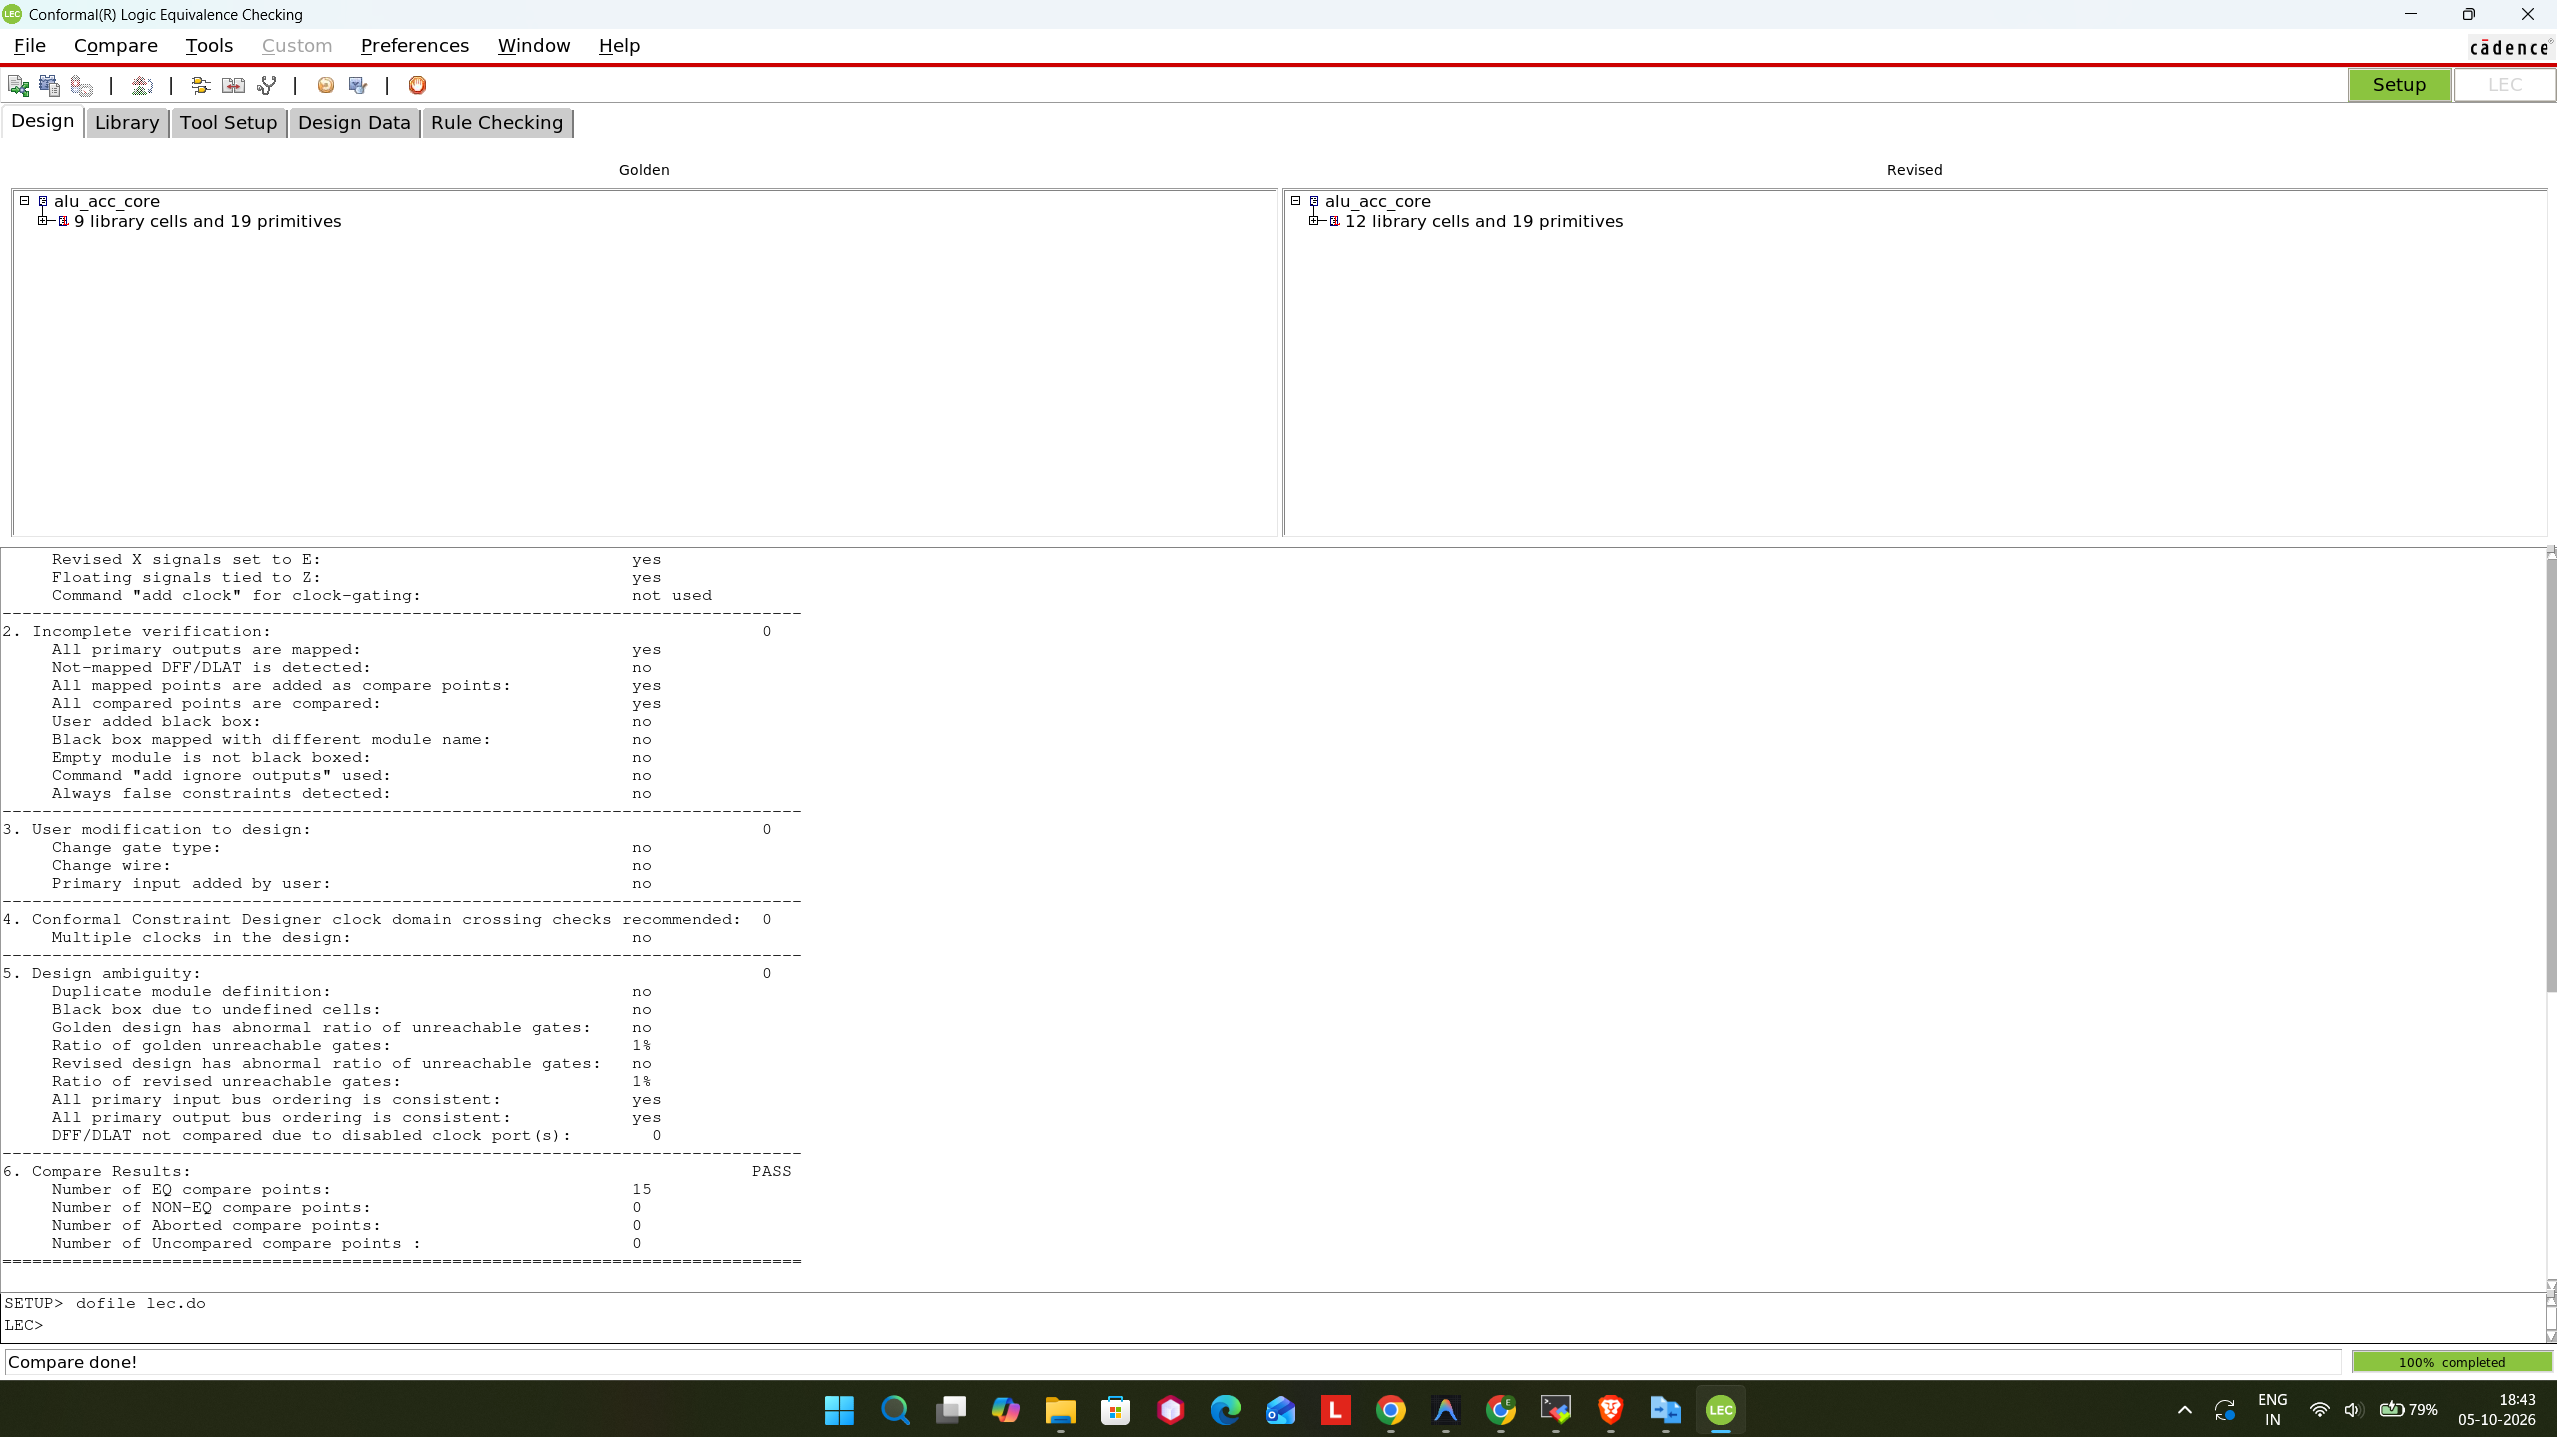
\includegraphics[width=0.8\textwidth]{Lab5_LEC_Exercises/Task6/output_after_correcting_task6.png}
    \caption{Task 6 - PASS after correction}
\end{figure}


% --- TASK 7 ---
\section{Task 7: Bad Clock Gating}
\textbf{Objective:} Identify equivalence failures caused by manually implemented clock gating.

\textbf{Diagnosis:} 
All 4 flip-flops failed. The designer attempted to implement clock gating using an AND gate (\texttt{assign gated\_clk = clk \& en}).

\begin{figure}[H]
    \centering
    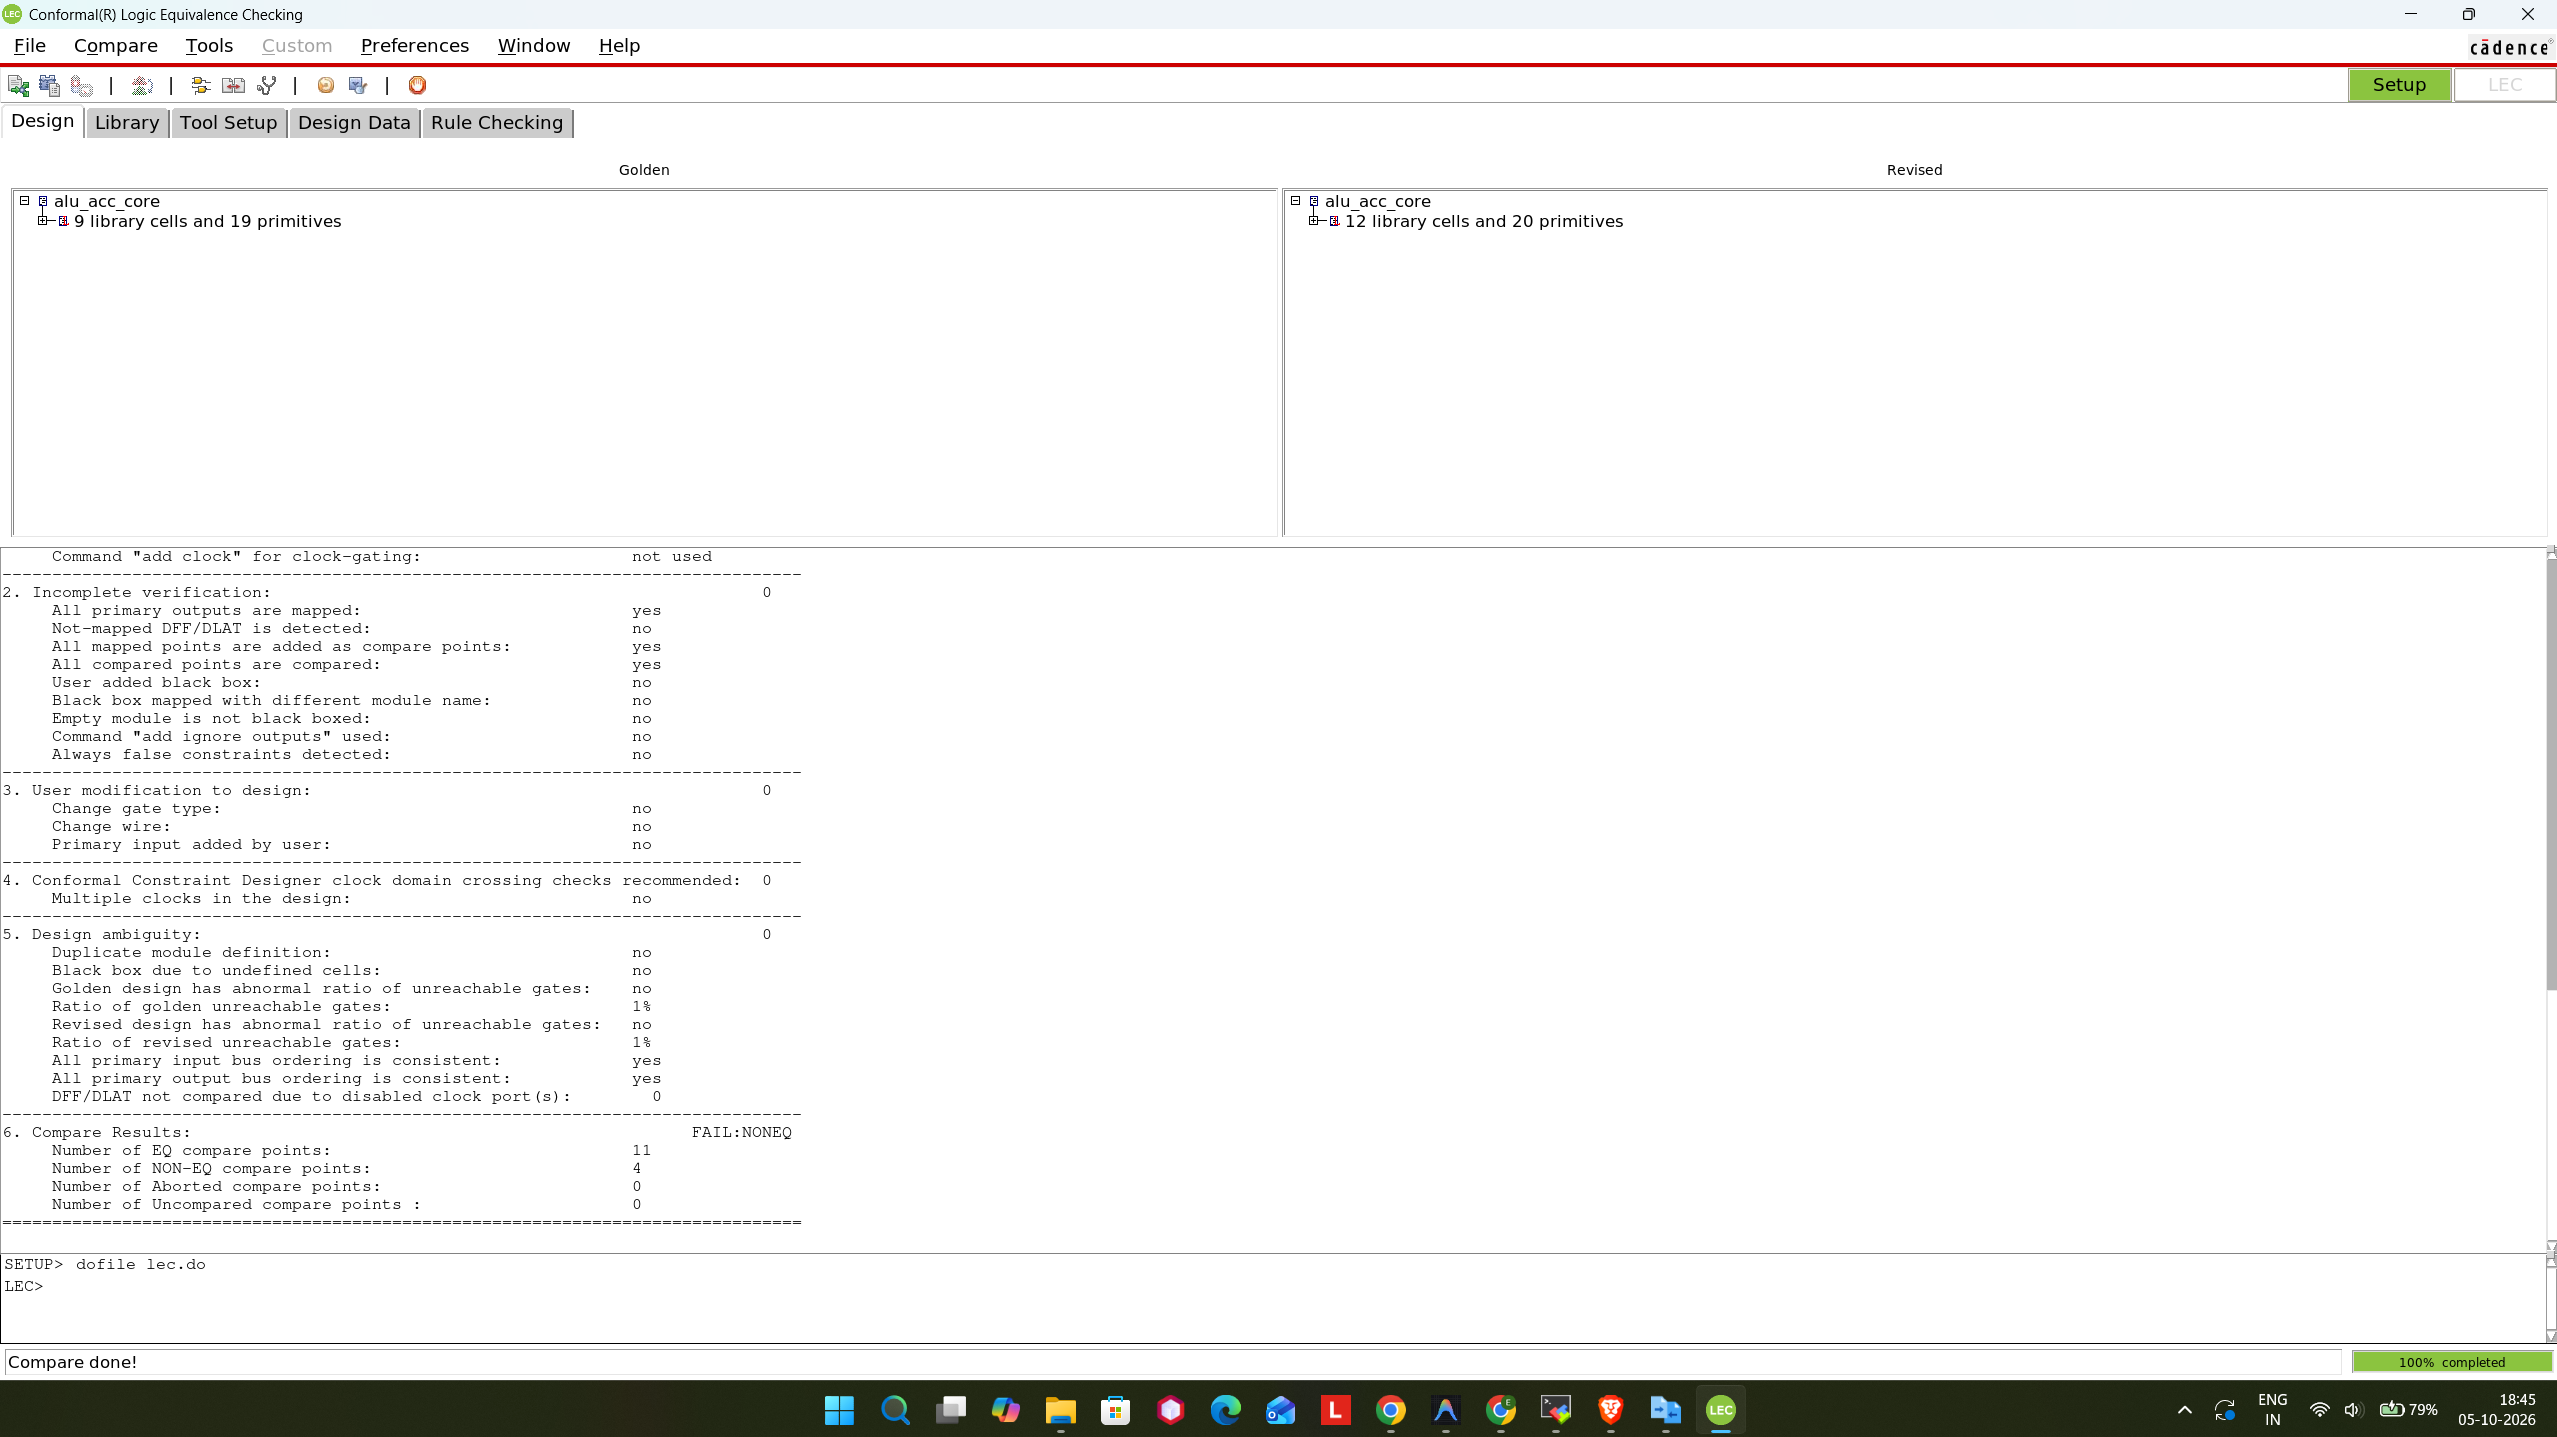
\includegraphics[width=0.8\textwidth]{Lab5_LEC_Exercises/Task7/output_task7.png}
    \caption{Task 7 - Initial Failure}
\end{figure}
\begin{figure}[H]
    \centering
    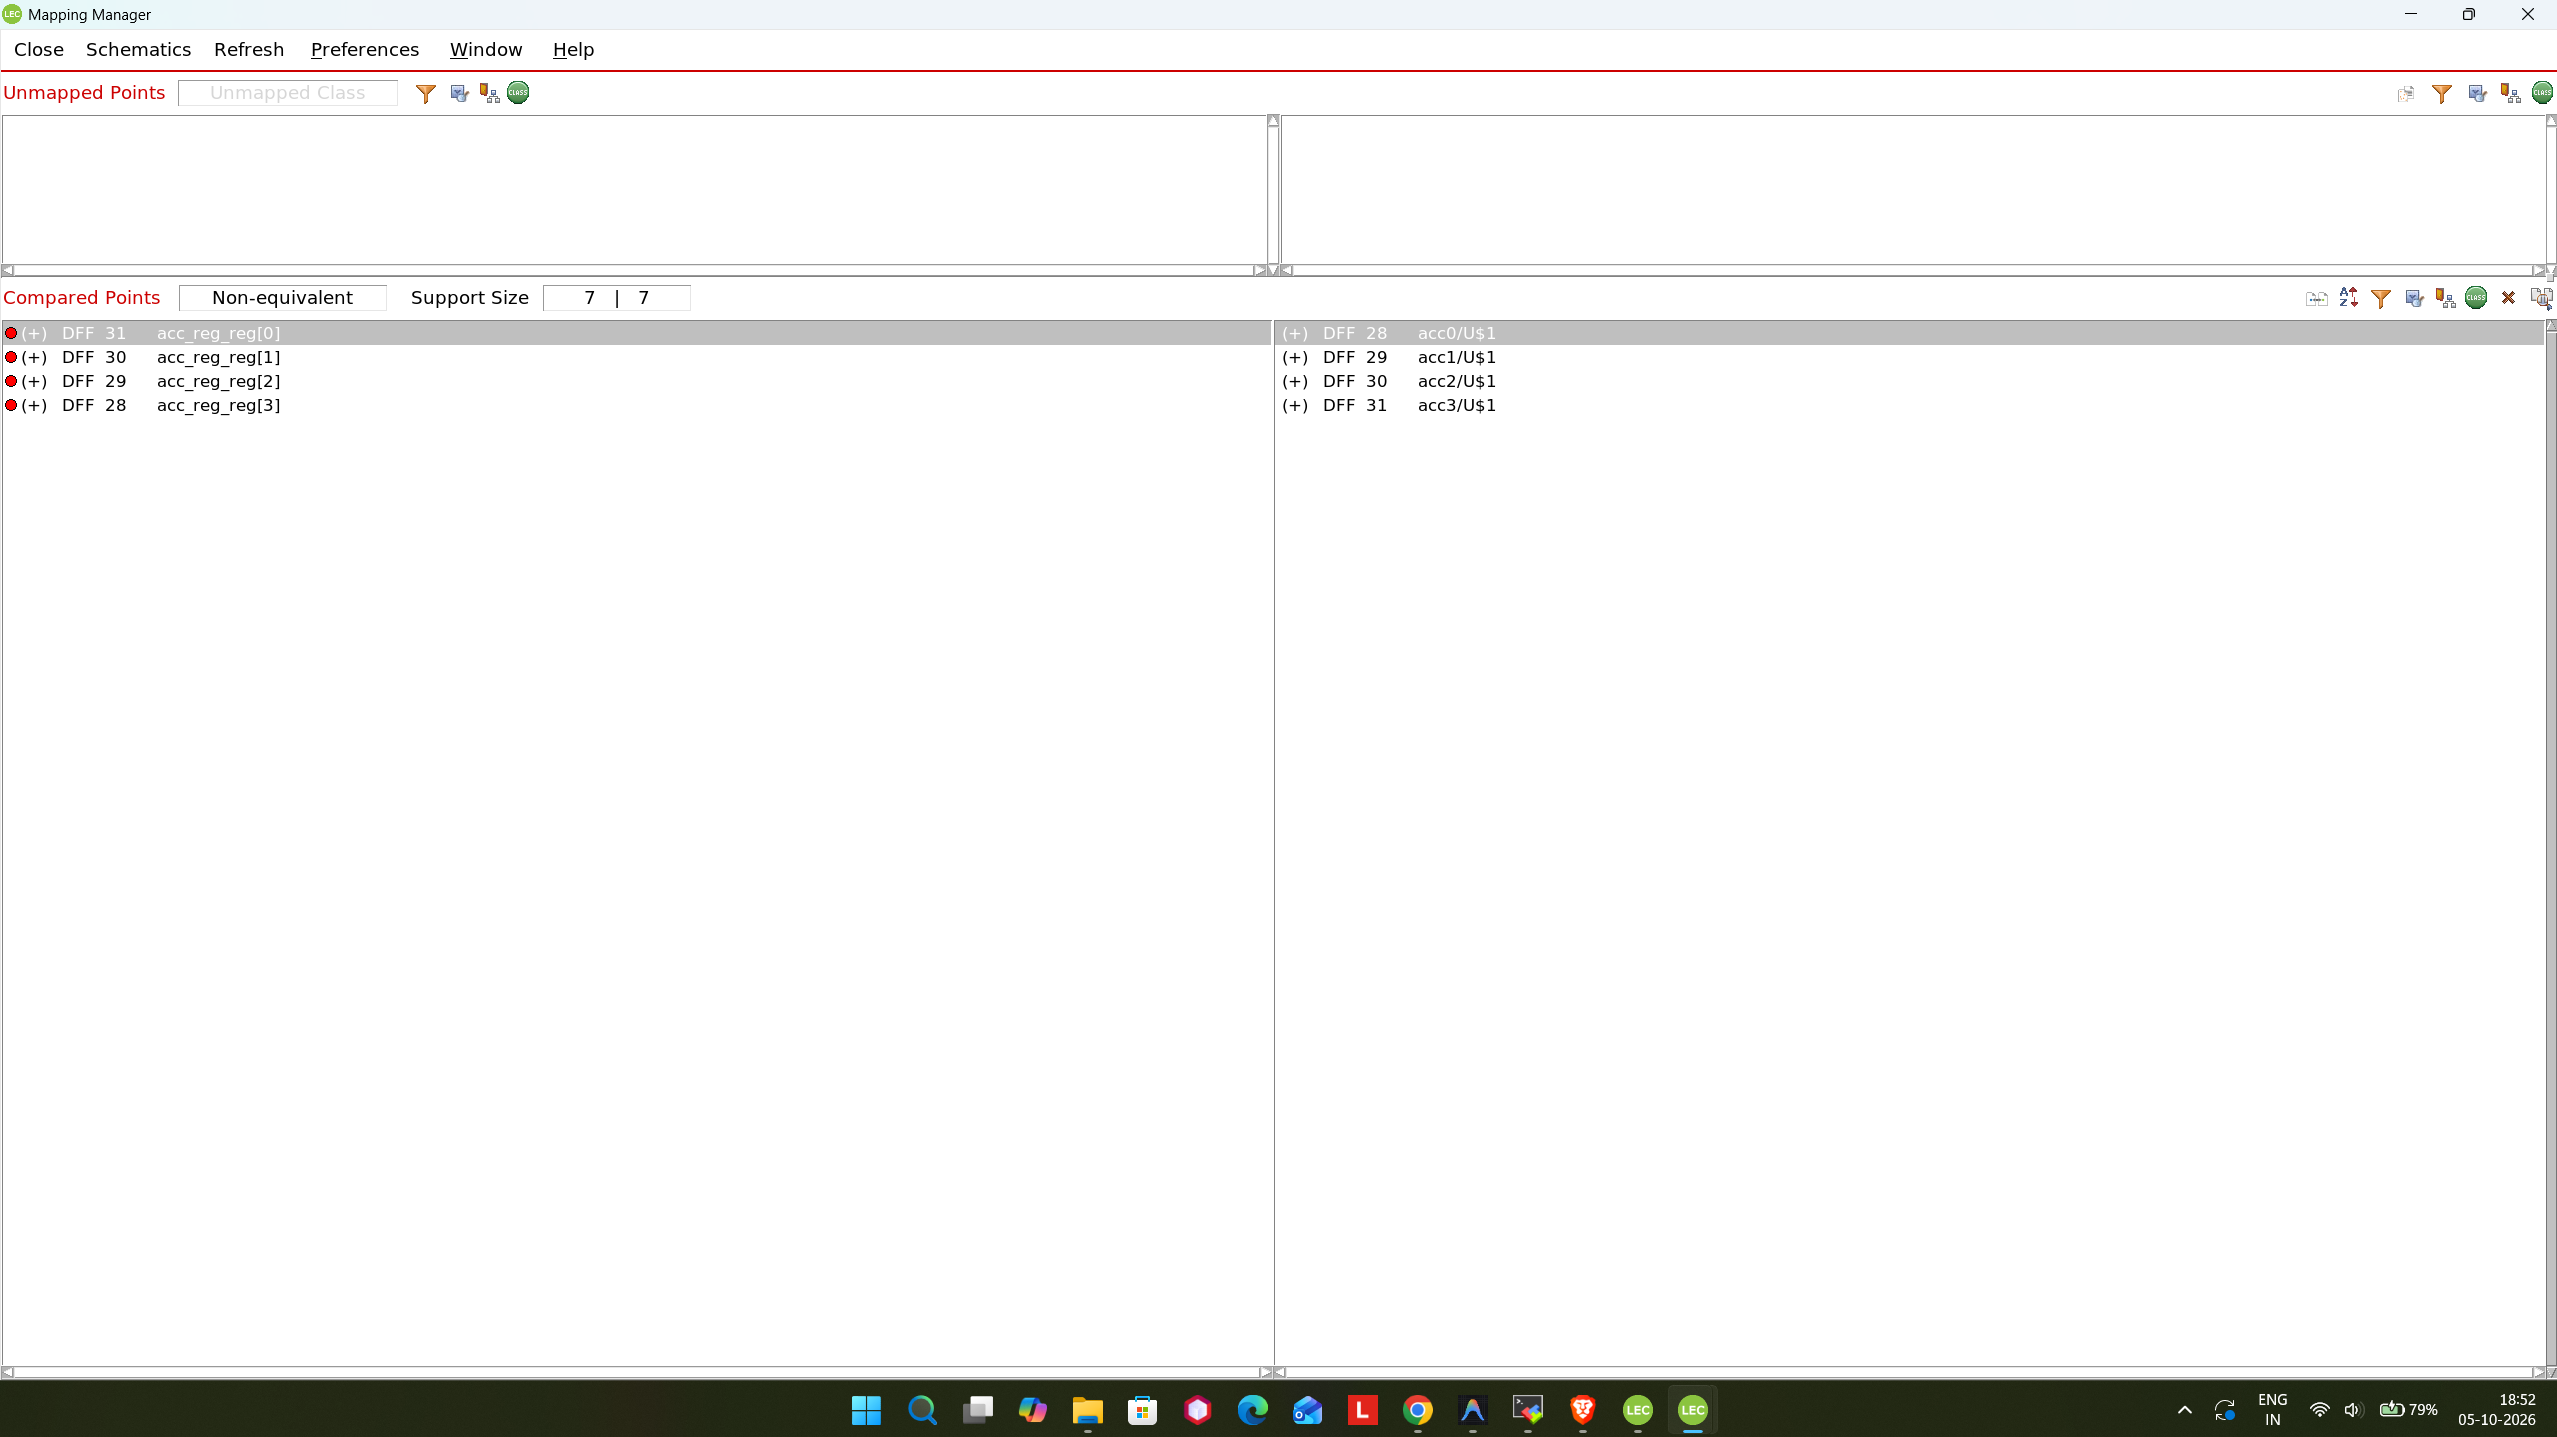
\includegraphics[width=0.8\textwidth]{Lab5_LEC_Exercises/Task7/mapping_manager_task7.png}
    \caption{Task 7 - Mapping Manager showing all DFFs failed}
\end{figure}
\begin{figure}[H]
    \centering
    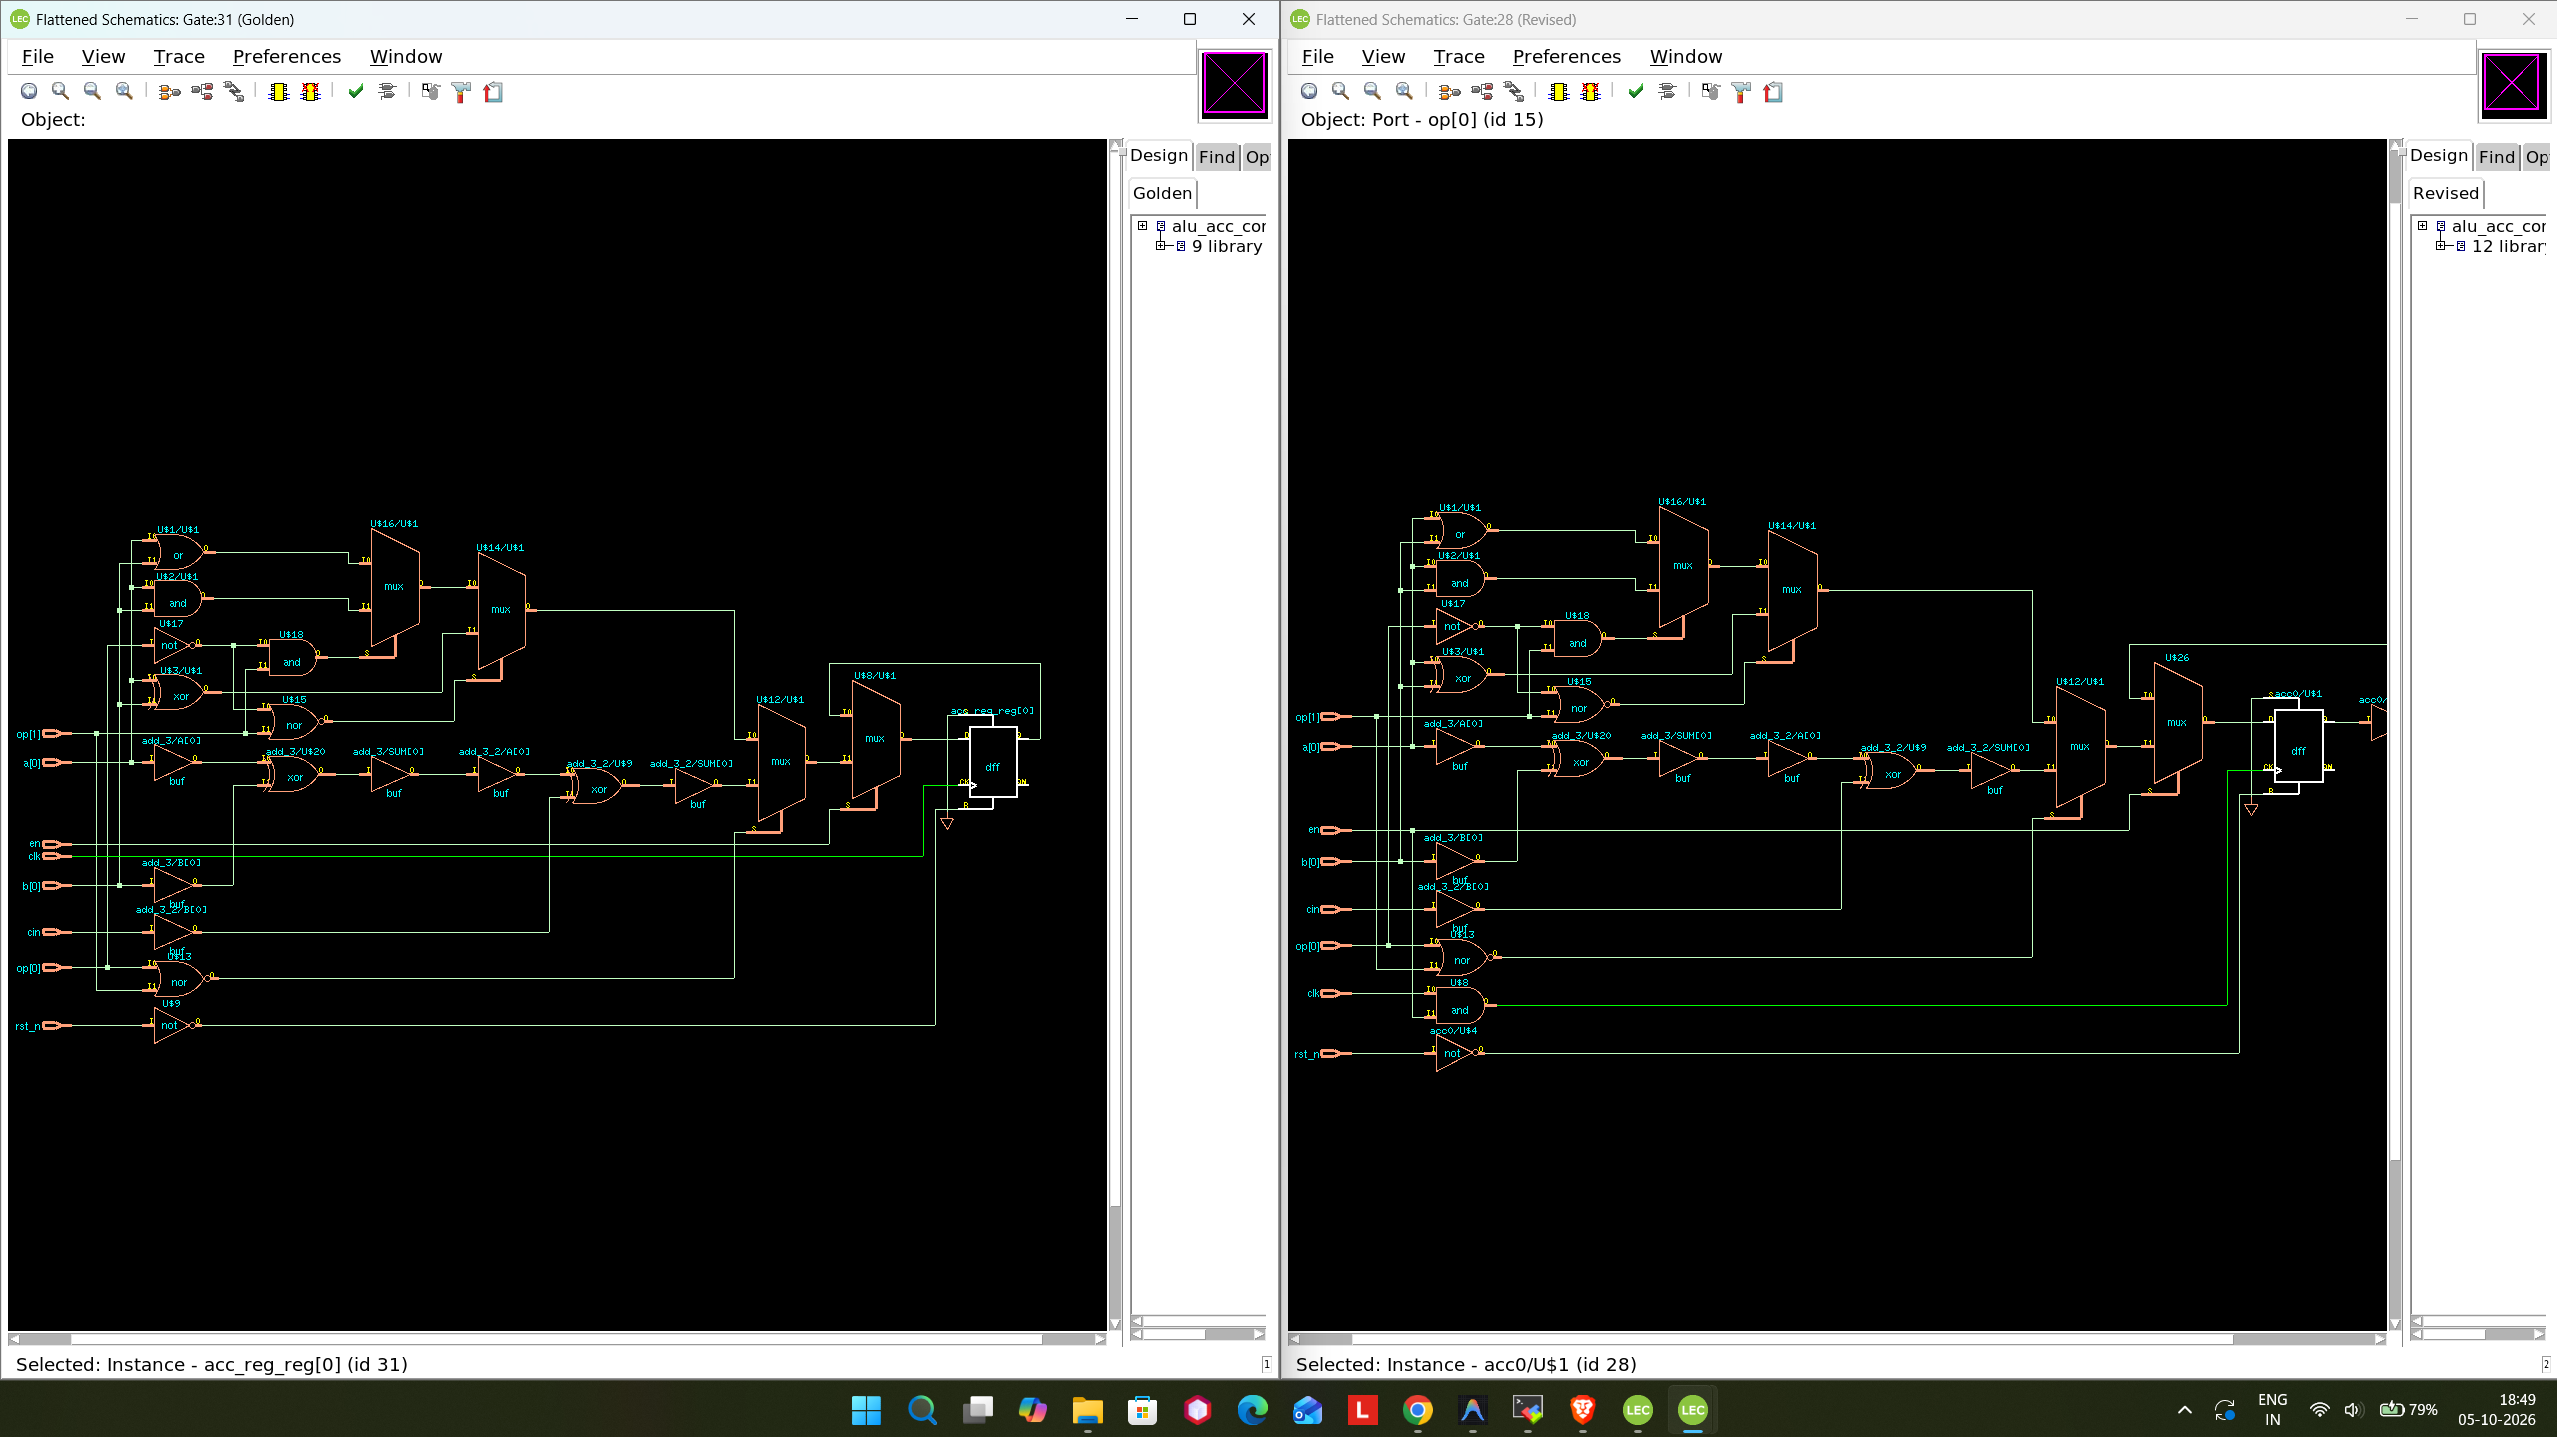
\includegraphics[width=0.8\textwidth]{Lab5_LEC_Exercises/Task7/schematic_task7.png}
    \caption{Task 7 - Schematic showing bad clock gating AND gate}
\end{figure}

\textbf{Correction:} 
The clock gating was bypassed to match the golden design.
\begin{lstlisting}[language=Verilog]
// Corrected Code:
assign gated_clk=clk;
\end{lstlisting}

\begin{figure}[H]
    \centering
    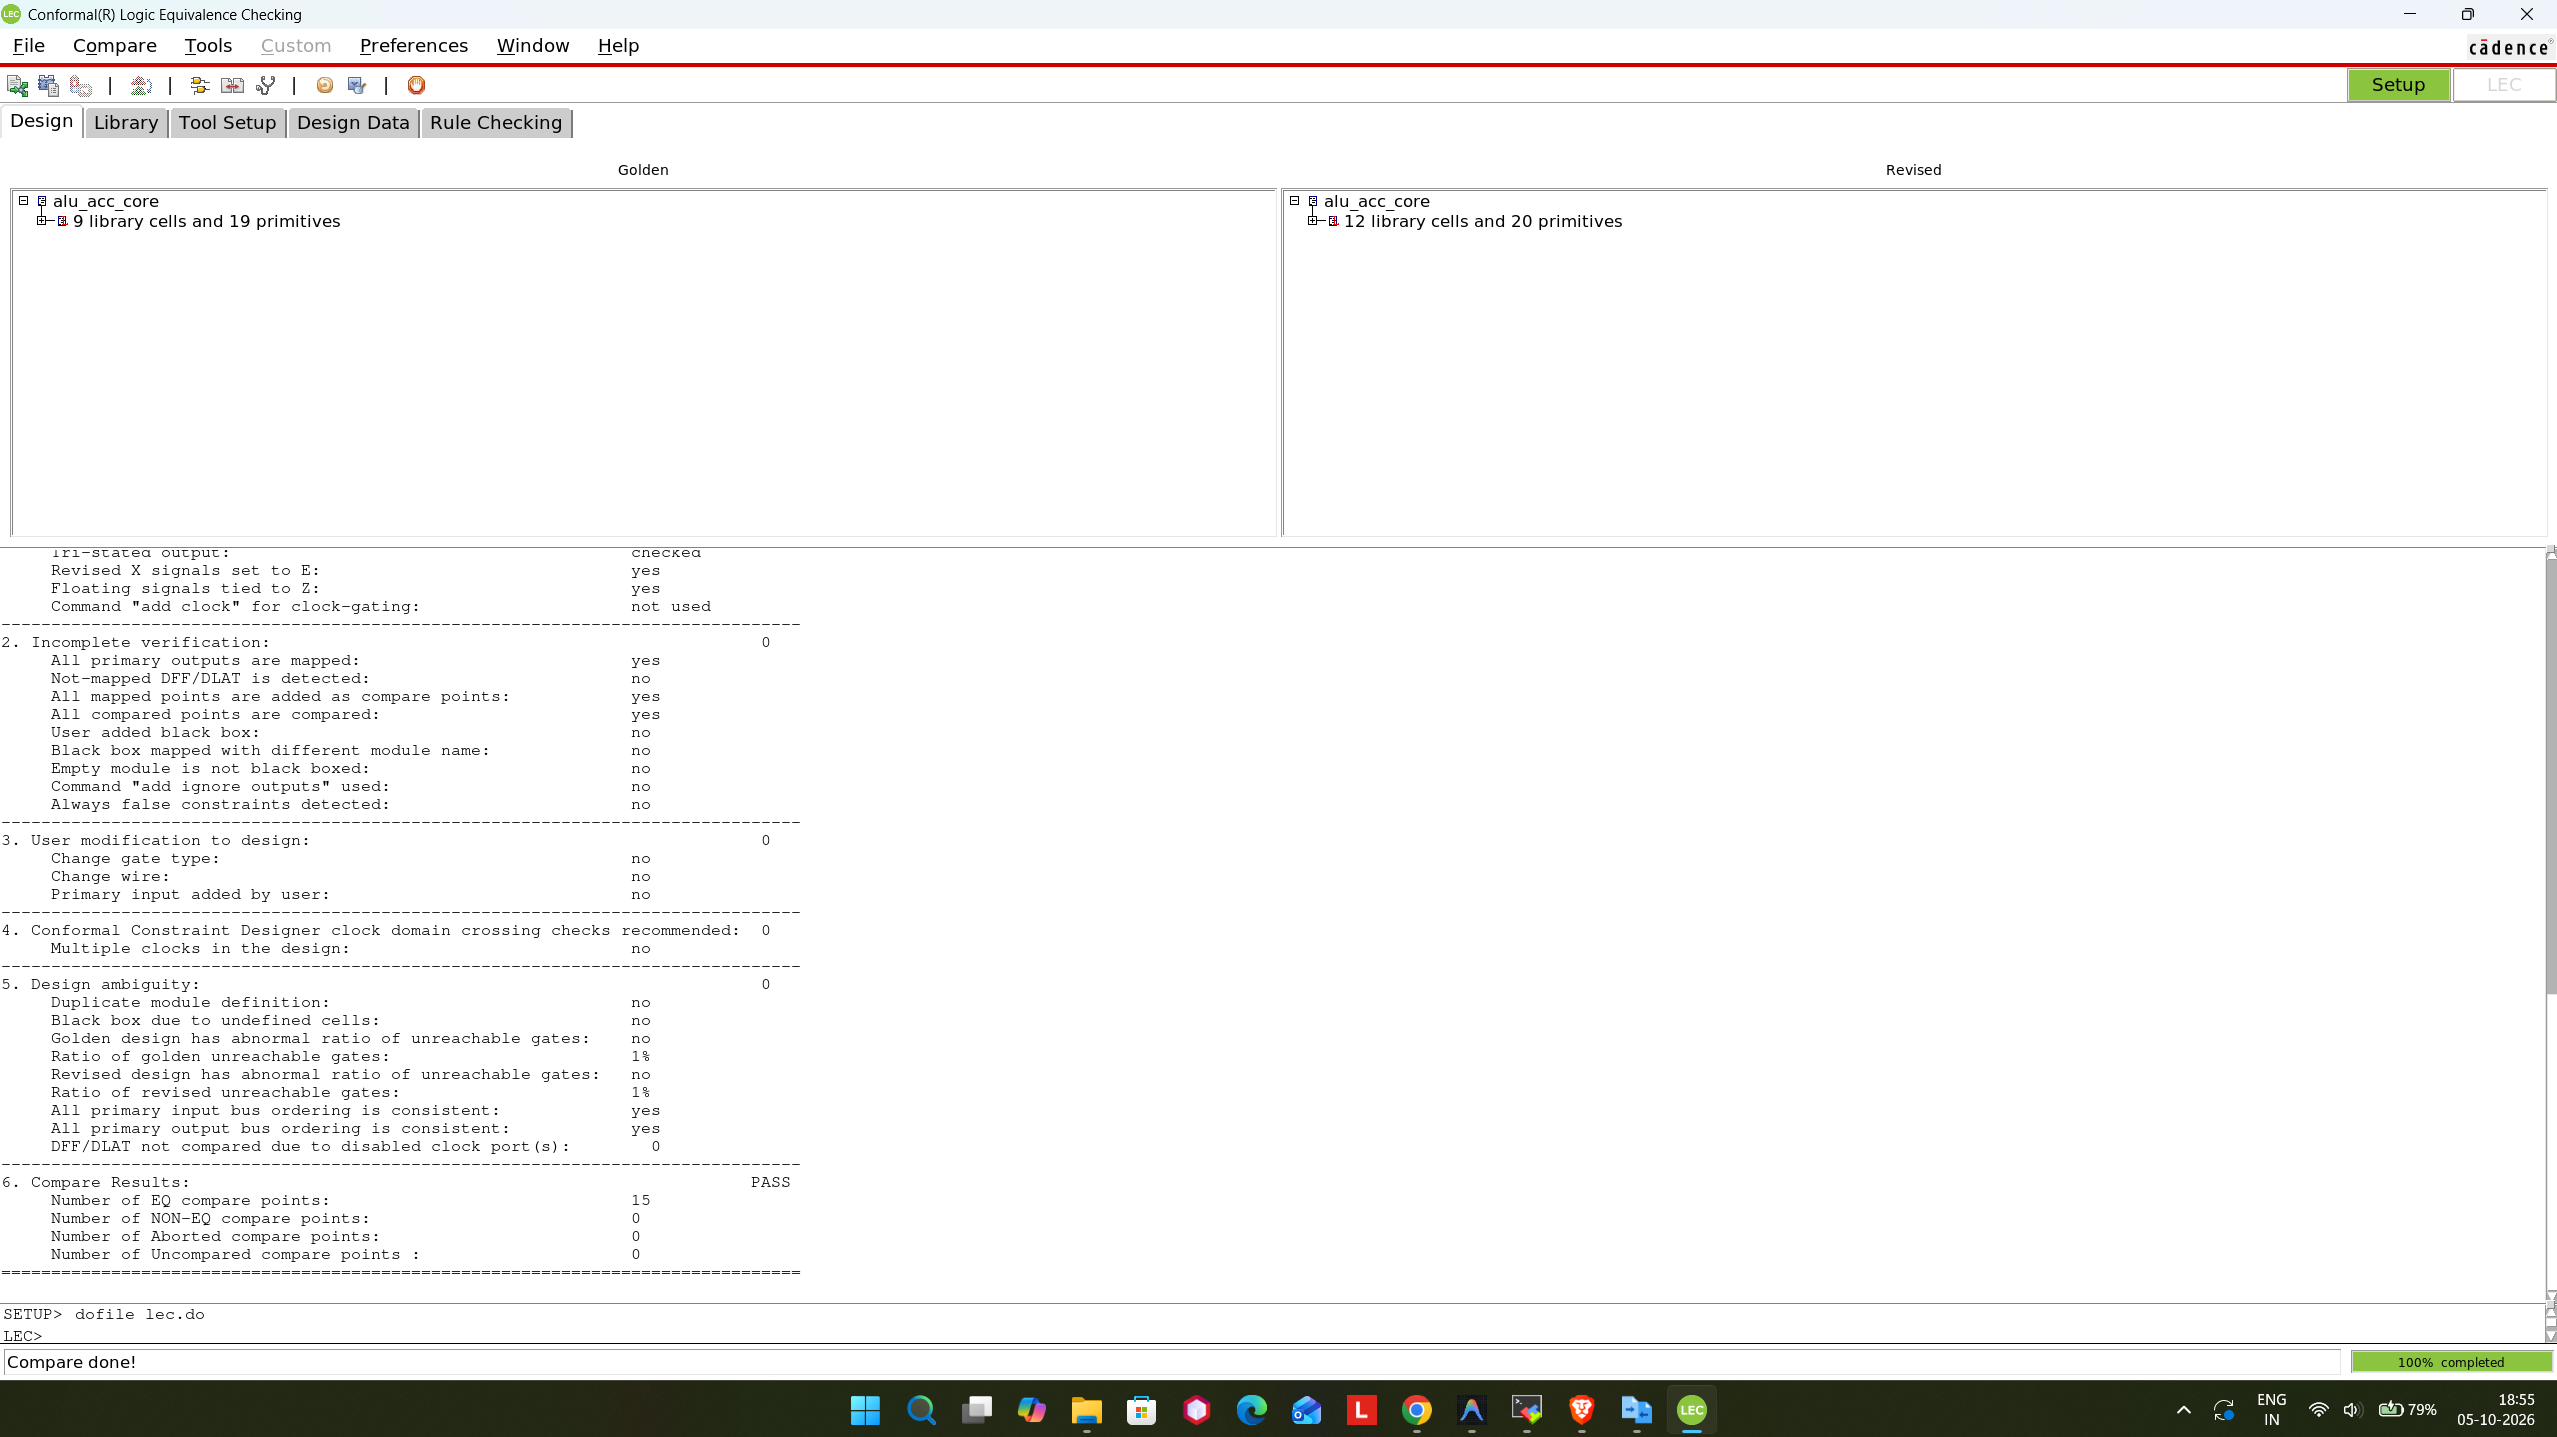
\includegraphics[width=0.8\textwidth]{Lab5_LEC_Exercises/Task7/output_after_correction.png}
    \caption{Task 7 - PASS after correction}
\end{figure}


% --- TASK 8 ---
\section{Task 8: Renamed Internal Wires (Unmapped Points)}
\textbf{Objective:} Understand structural mapping capabilities in Conformal.

\textbf{Diagnosis:} 
The designer renamed \texttt{acc\_reg} to \texttt{accumulator\_reg}. Conformal's structural mapping algorithms successfully mapped the logic cones and passed the design because it is logically identical.

\begin{figure}[H]
    \centering
    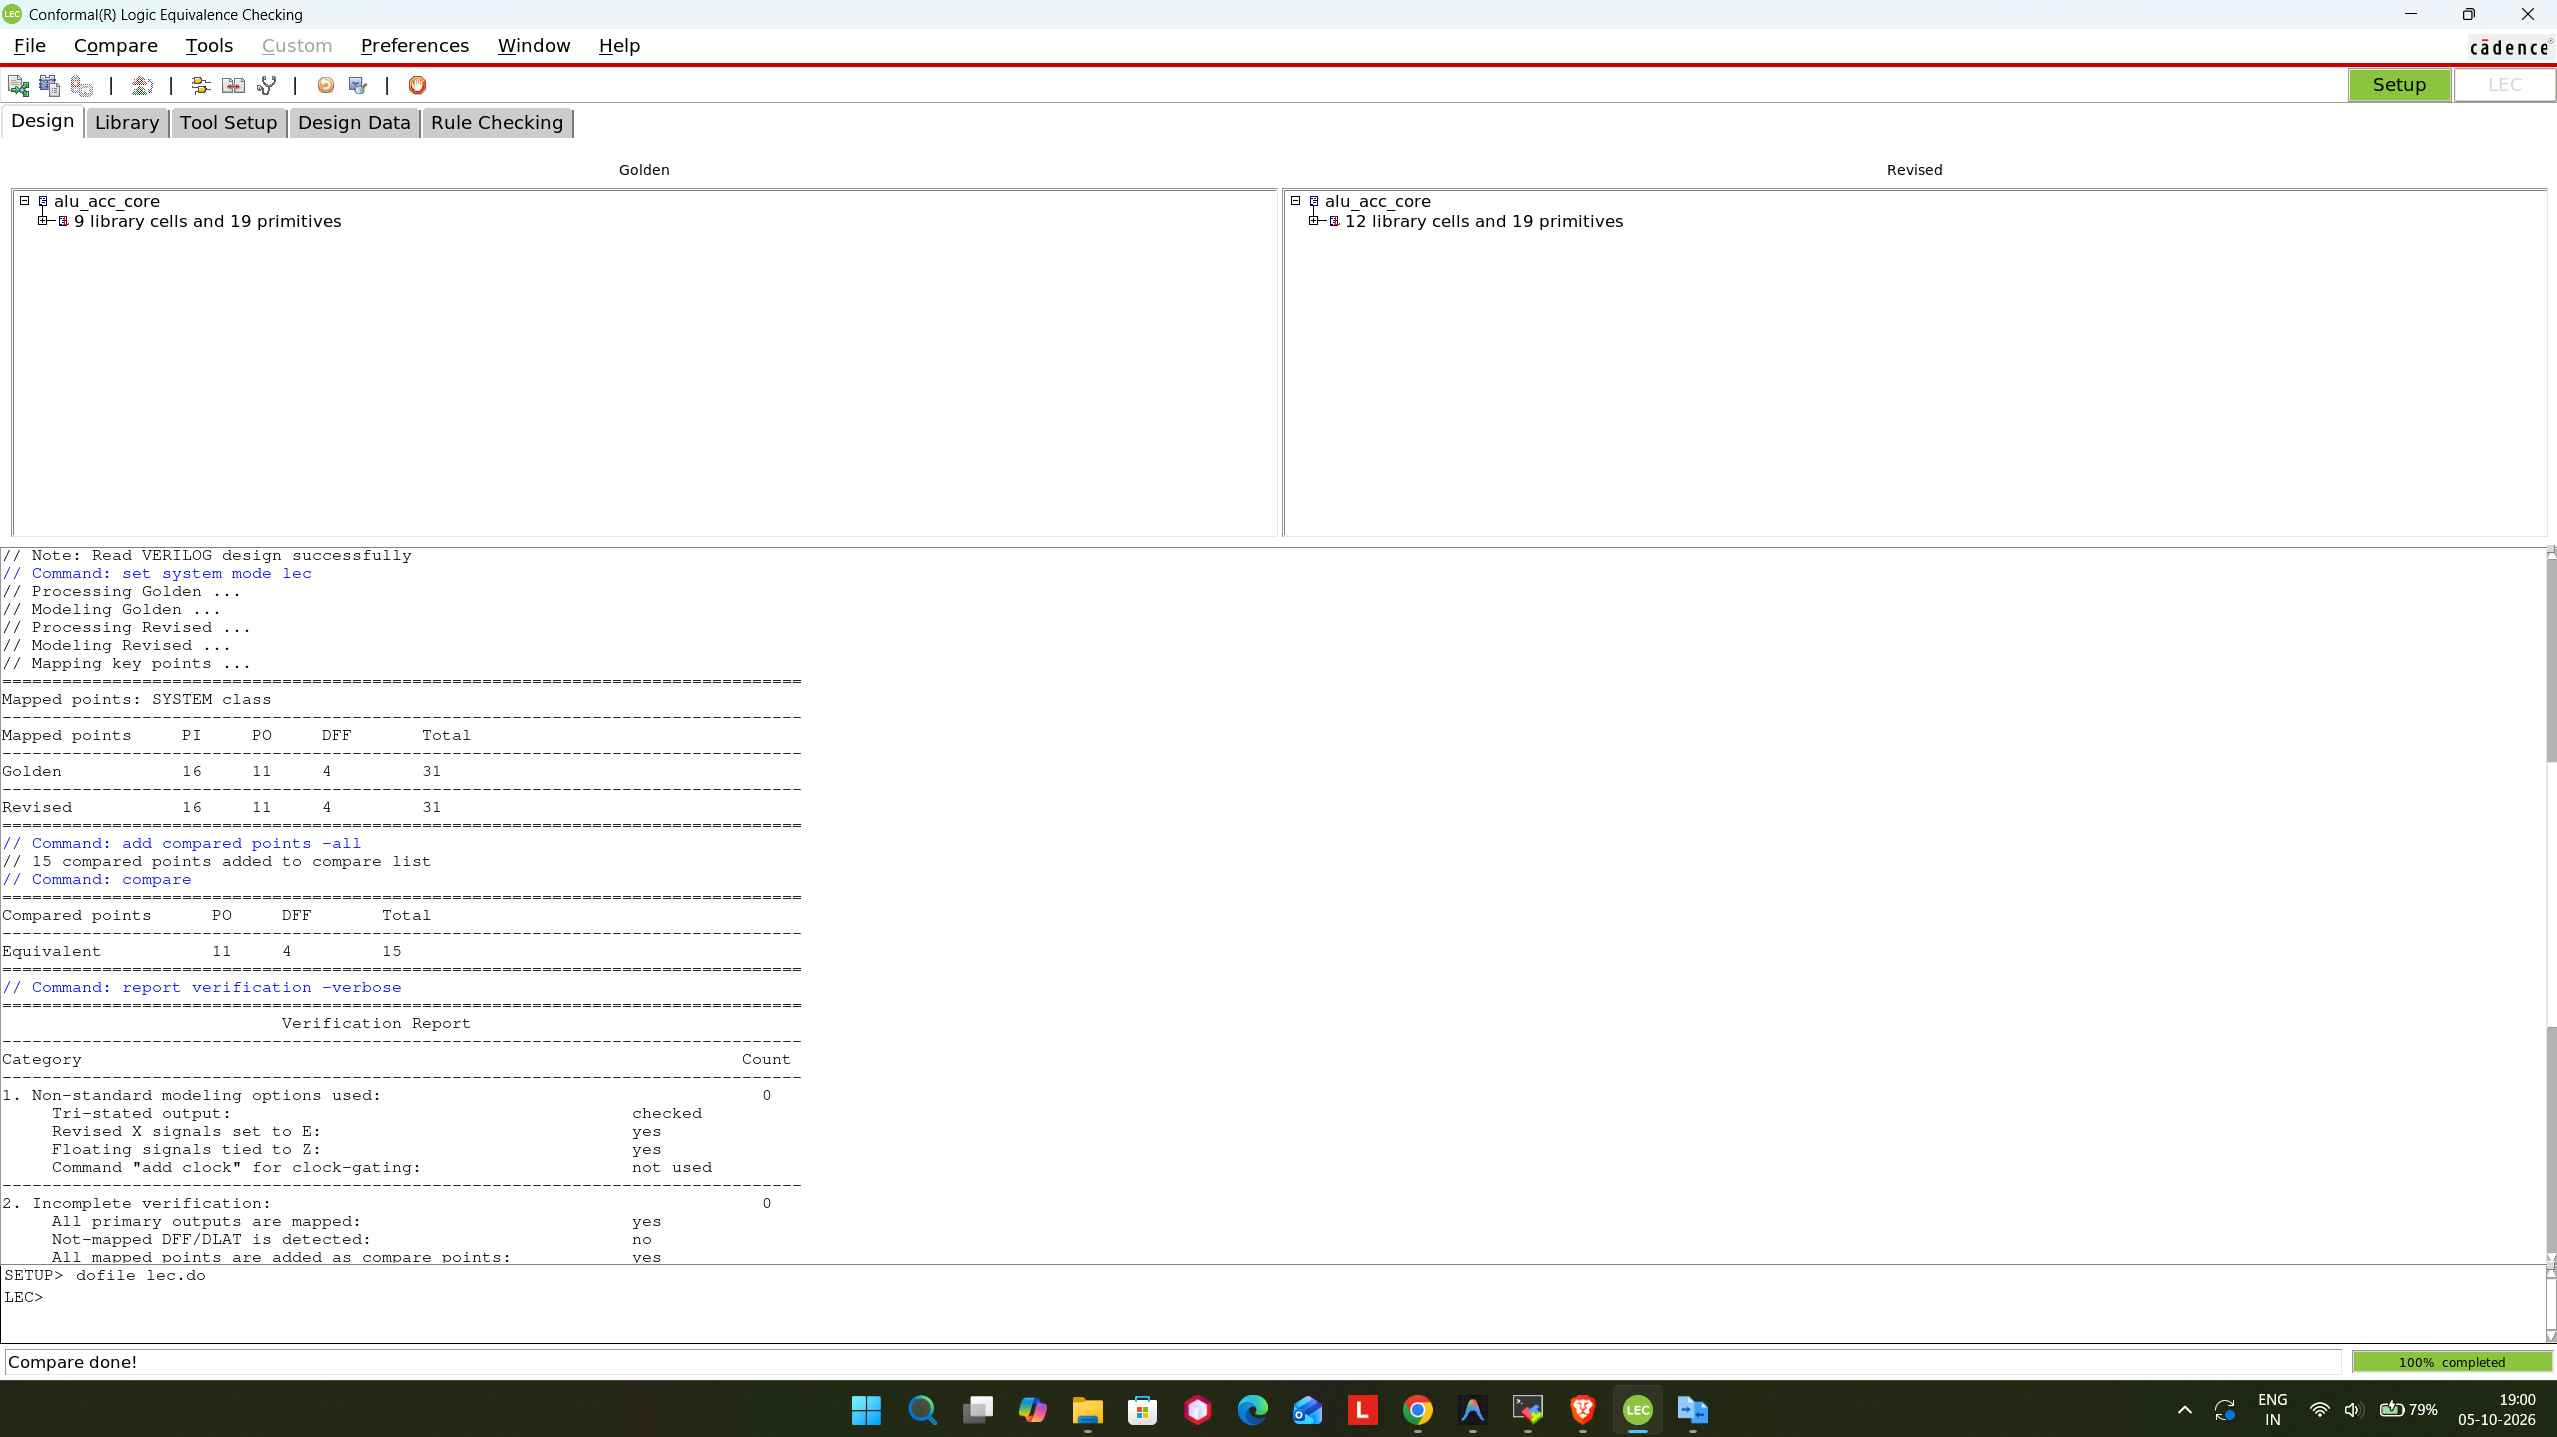
\includegraphics[width=0.8\textwidth]{Lab5_LEC_Exercises/Task8/output_task8.png}
    \caption{Task 8 - PASS with Structural Mapping despite renamed wires}
\end{figure}


% --- TASK 9 ---
\section{Task 9: Corrupted Combinational Logic}
\textbf{Objective:} Debug a hardcoded bit failure deep within the combinational logic cone.

\textbf{Diagnosis:} 
A cascading failure occurred on \texttt{result[2]}, \texttt{zero}, and \texttt{acc\_reg[2]}. The designer hardcoded bit 2 of the AND operation.

\begin{figure}[H]
    \centering
    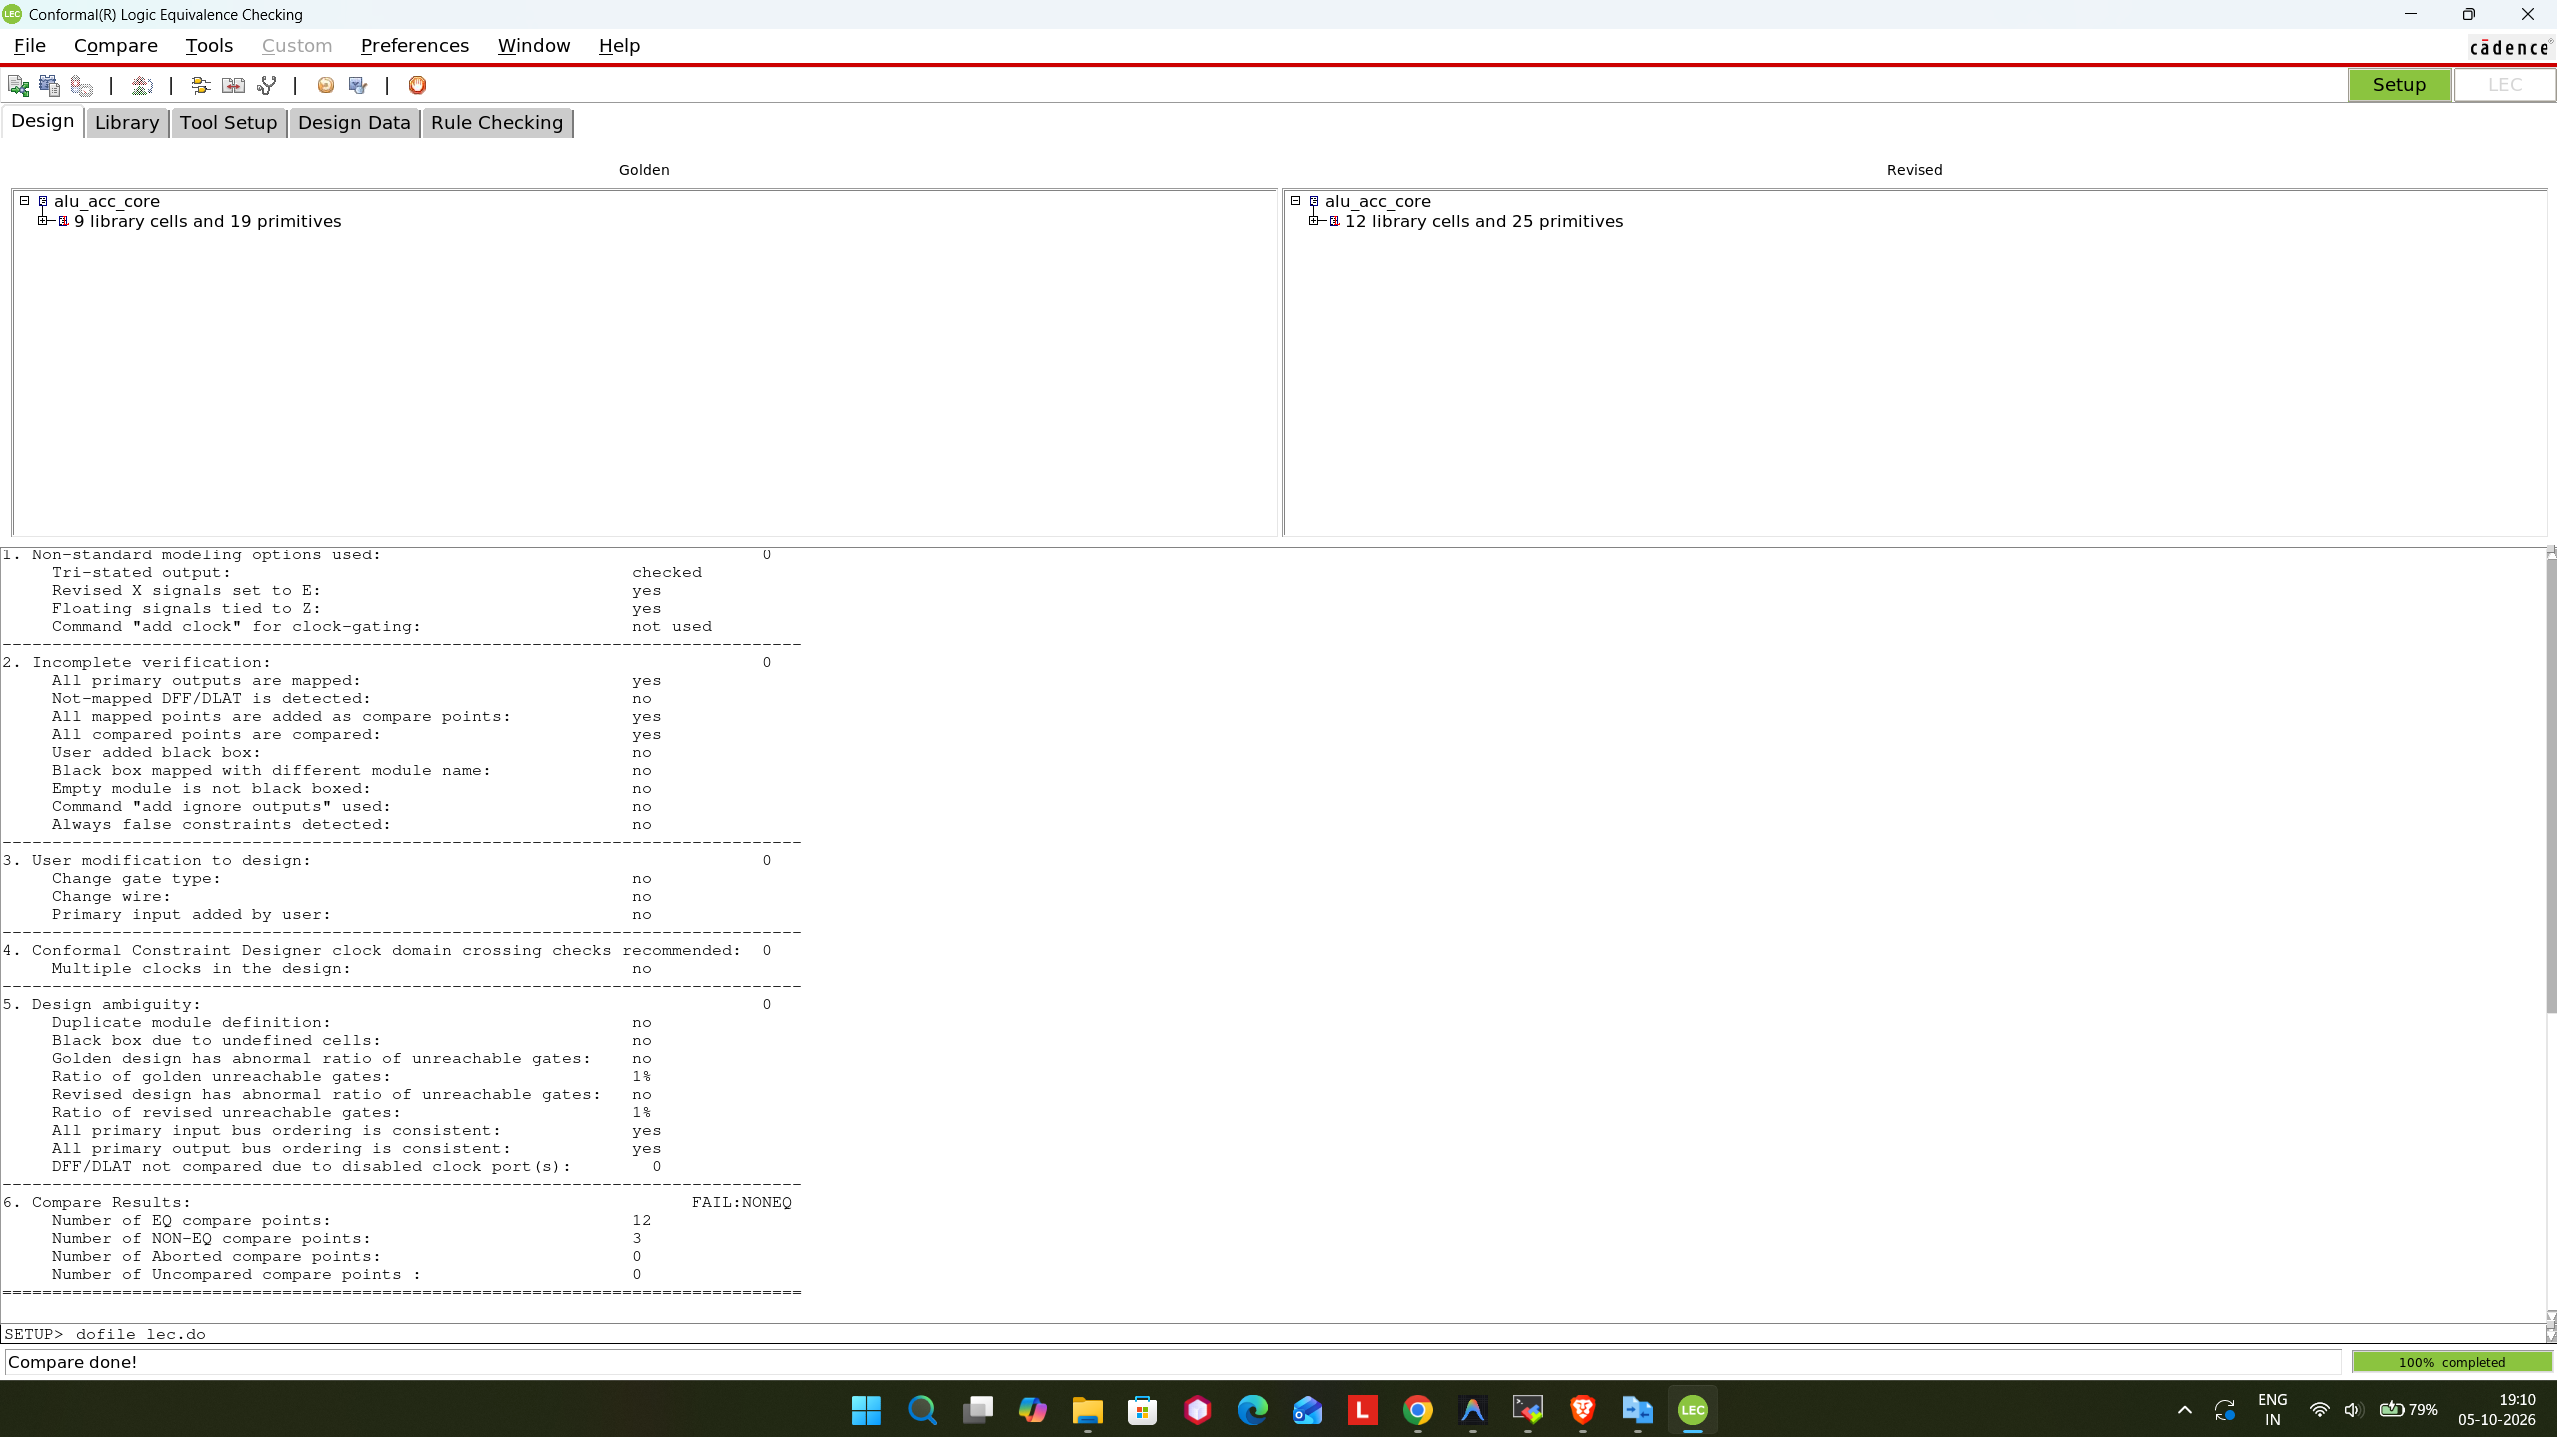
\includegraphics[width=0.8\textwidth]{Lab5_LEC_Exercises/Task9/output_task9.png}
    \caption{Task 9 - Initial Failure showing 3 cascading errors}
\end{figure}
\begin{figure}[H]
    \centering
    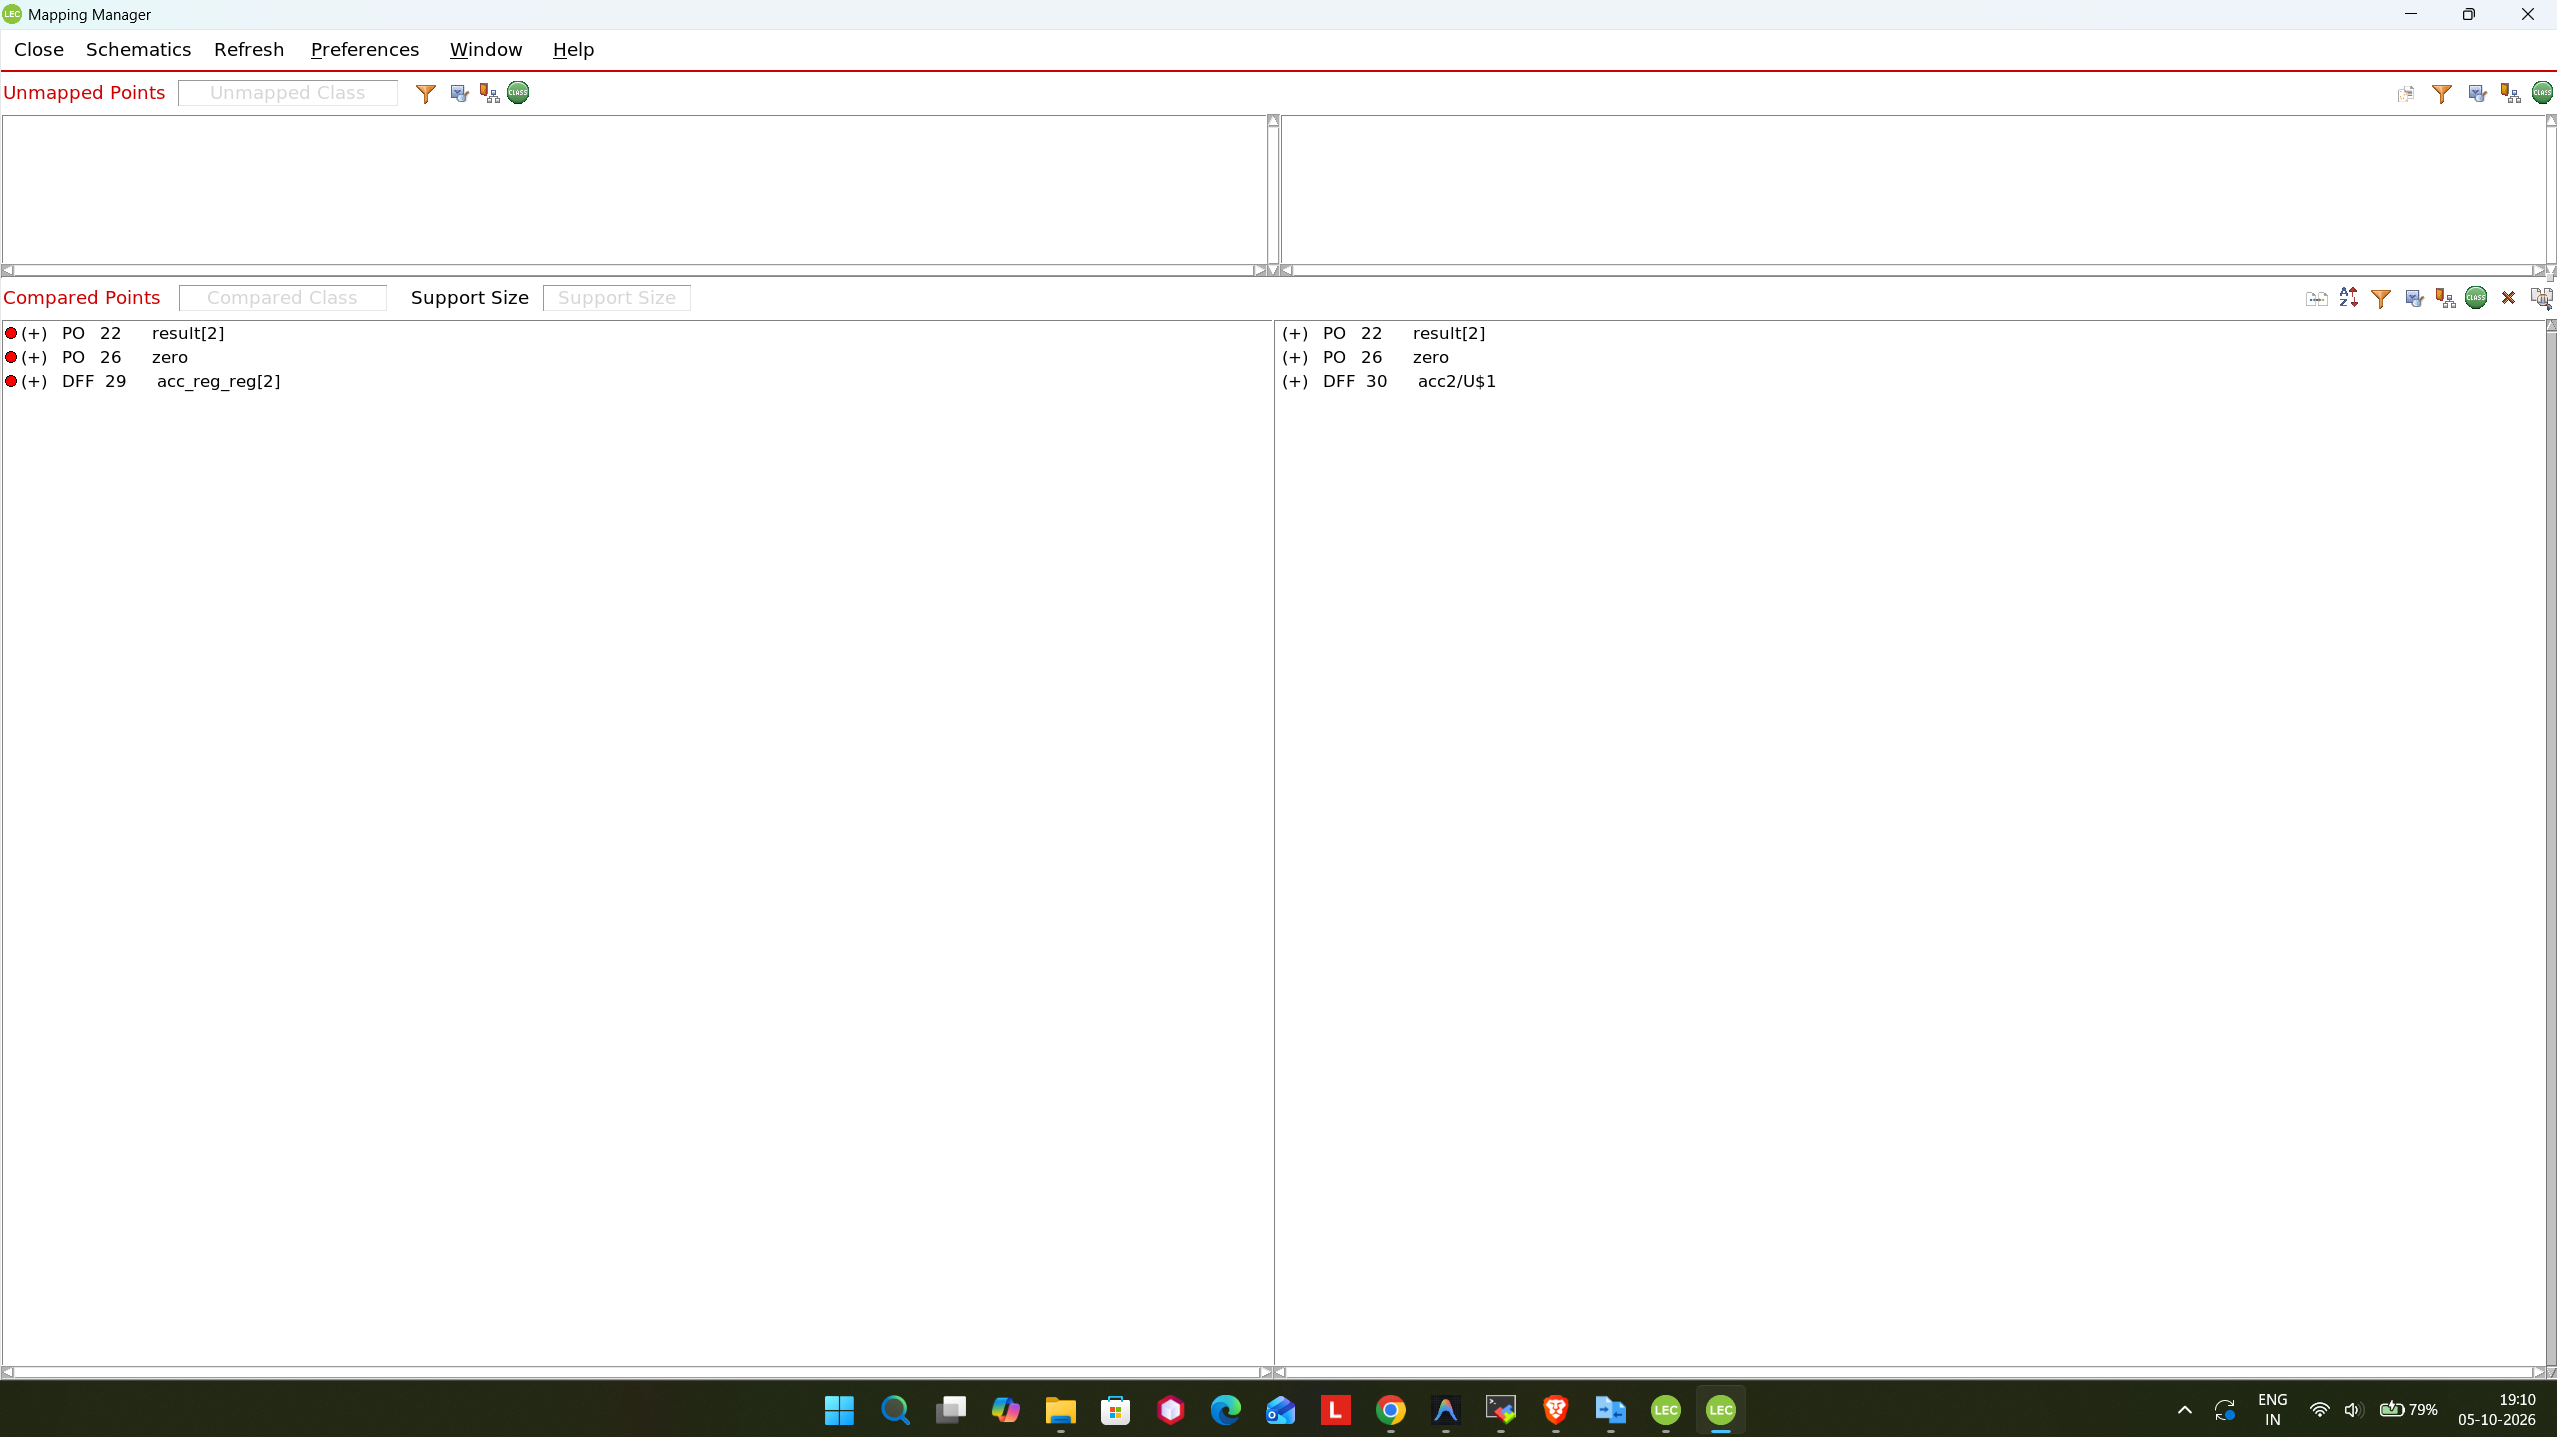
\includegraphics[width=0.8\textwidth]{Lab5_LEC_Exercises/Task9/mapping_manager_task9.png}
    \caption{Task 9 - Mapping Manager}
\end{figure}

\textbf{Correction:} 
The redundant logic was deleted.
\begin{lstlisting}[language=Verilog]
// Corrected Code:
assign and_r=a&b; assign or_r=a|b;
\end{lstlisting}

\begin{figure}[H]
    \centering
    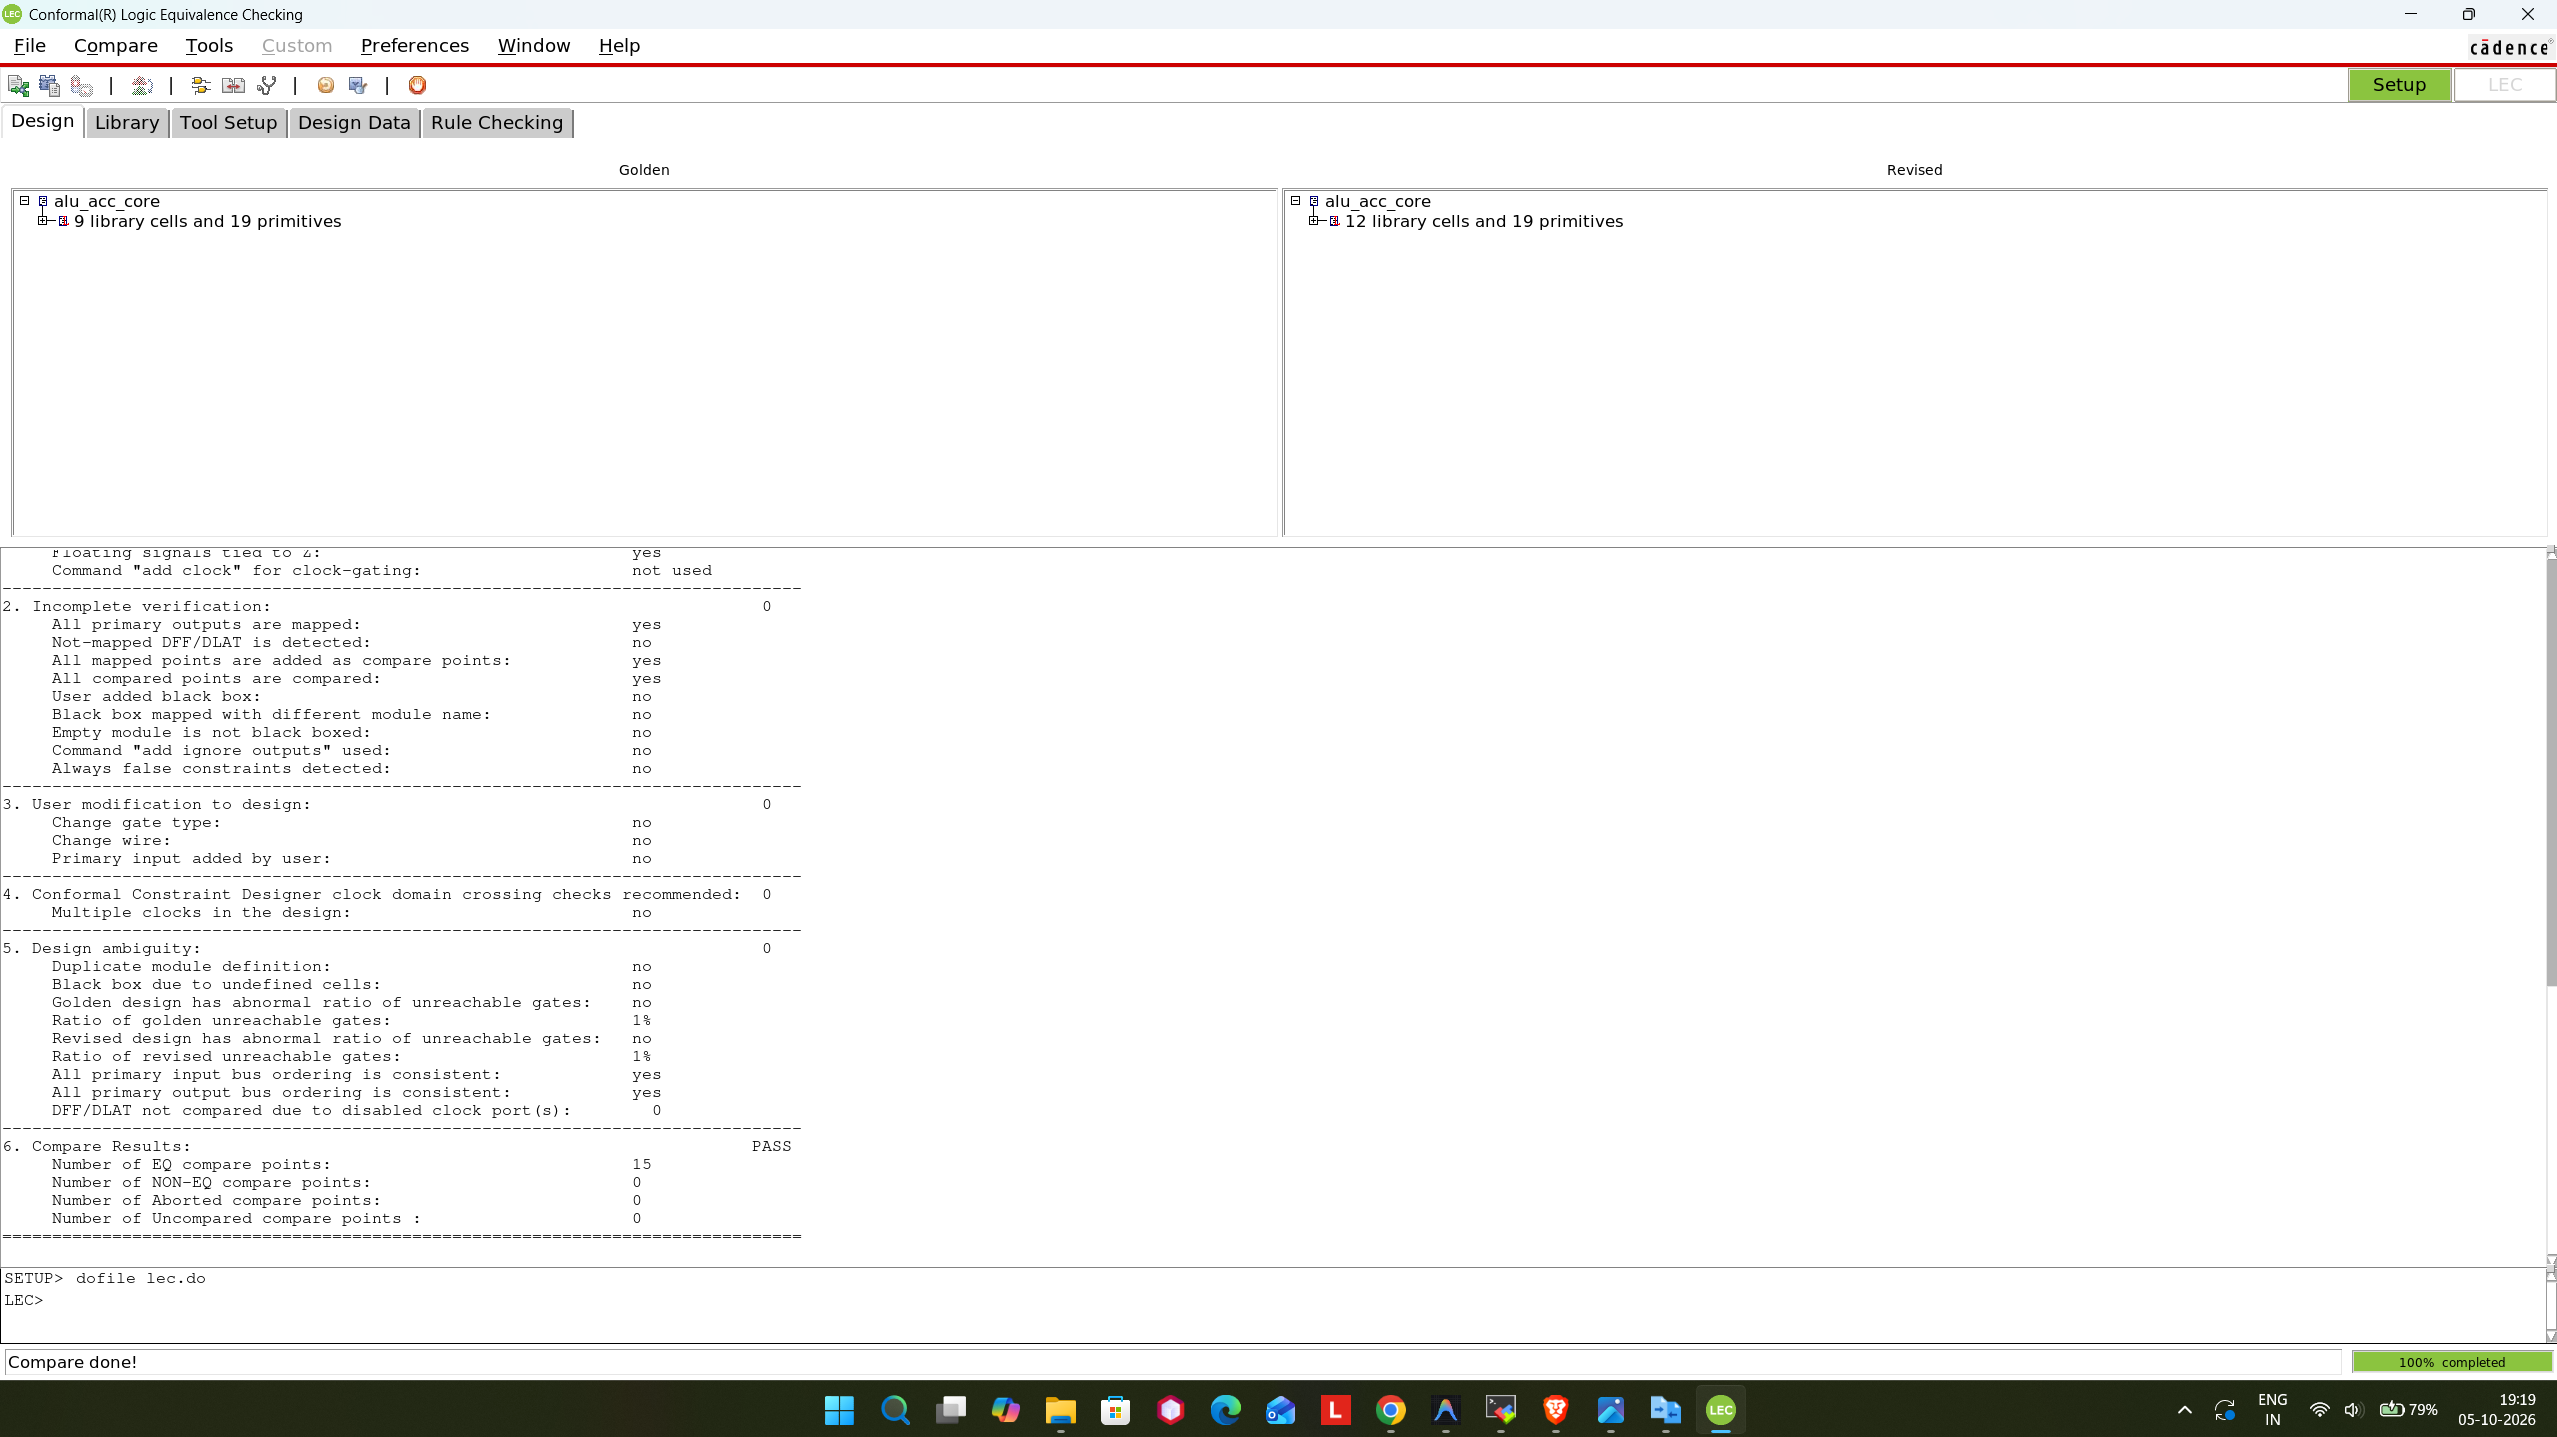
\includegraphics[width=0.8\textwidth]{Lab5_LEC_Exercises/Task9/output_after_correcting_task9.png}
    \caption{Task 9 - PASS after correction}
\end{figure}

\end{document}
